%%%%%%%%%%%%%%%%%%%%%%%%%%%%%%%%%%%%%%%%%
% Masters/Doctoral Thesis 
% LaTeX Template
% Version 1.43 (17/5/14)
%
% This template has been downloaded from:
% http://www.LaTeXTemplates.com
%
% Original authors:
% Steven Gunn 
% http://users.ecs.soton.ac.uk/srg/softwaretools/document/templates/
% and
% Sunil Patel
% http://www.sunilpatel.co.uk/thesis-template/
%
% License:
% CC BY-NC-SA 3.0 (http://creativecommons.org/licenses/by-nc-sa/3.0/)
%
% Note:
% Make sure to edit document variables in the Thesis.cls file
%
%%%%%%%%%%%%%%%%%%%%%%%%%%%%%%%%%%%%%%%%%

%----------------------------------------------------------------------------------------
%	PACKAGES AND OTHER DOCUMENT CONFIGURATIONS
%----------------------------------------------------------------------------------------

%\documentclass[11pt, oneside]{Thesis} % The default font size and one-sided printing (no margin offsets)
\documentclass[11pt, openright]{Thesis} % The default font size and one-sided printing (no margin offsets)

\graphicspath{{assets/}} % Specifies the directory where pictures are stored

\usepackage[square, numbers, comma, sort&compress]{natbib} % Use the natbib reference package - read up on this to edit the reference style; if you want text (e.g. Smith et al., 2012) for the in-text references (instead of numbers), remove 'numbers' 
%%%%%%%%%
\usepackage{amsmath,amsfonts,amsthm,amssymb}
\usepackage[usenames,dvipsnames]{xcolor}
\usepackage{setspace}
\usepackage{Tabbing}
\usepackage{fancyhdr}
\usepackage{lastpage}
\usepackage{extramarks}
\usepackage{chngpage}
\usepackage{soul,color}
\usepackage{graphicx,float,wrapfig}
\usepackage{times}
\usepackage{tabularx,ragged2e}
\usepackage{booktabs}
\usepackage{natbib}
\usepackage{epstopdf}
\usepackage{caption}
\usepackage{subcaption}
\usepackage[english]{babel}
\usepackage{lscape}
\usepackage{tikz}
\usepackage[linesnumbered,ruled,vlined]{algorithm2e}
\usepackage{multirow}
\usepackage{listings}


\lstdefinelanguage{XML}
{
  basicstyle=\ttfamily\footnotesize,
  morestring=[b]",
  moredelim=[s][\bfseries\color{Maroon}]{<}{\ },
  moredelim=[s][\bfseries\color{Maroon}]{</}{>},
  moredelim=[l][\bfseries\color{Maroon}]{/>},
  moredelim=[l][\bfseries\color{Maroon}]{>},
  morecomment=[s]{<?}{?>},
  morecomment=[s]{<!--}{-->},
  commentstyle=\color{Maroon},
  stringstyle=\color{blue},
  identifierstyle=\color{red}
}

%\usepackage{url}
%\usepackage{hyperref}
%%%%%%%%%%
\hypersetup{urlcolor=blue, colorlinks=true} % Colors hyperlinks in blue - change to black if annoying
\title{\ttitle} % Defines the thesis title - don't touch this

\begin{document}

\frontmatter % Use roman page numbering style (i, ii, iii, iv...) for the pre-content pages

\setstretch{1.3} % Line spacing of 1.3

% Define the page headers using the FancyHdr package and set up for one-sided printing
\fancyhead{} % Clears all page headers and footers
\rhead{\thepage} % Sets the right side header to show the page number
\lhead{} % Clears the left side page header

\pagestyle{fancy} % Finally, use the "fancy" page style to implement the FancyHdr headers

\newcommand{\HRule}{\rule{\linewidth}{0.5mm}} % New command to make the lines in the title page

% PDF meta-data
\hypersetup{pdftitle={\ttitle}}
\hypersetup{pdfsubject=\subjectname}
\hypersetup{pdfauthor=\authornames}
\hypersetup{pdfkeywords=\keywordnames}

\newcommand{\eqdef}{=\mathrel{\mathop:}}
\newcommand{\argmin}{\mathop{\rm argmin}\limits}
\newcommand{\Tau}{\mathop{\text{\Large{$\tau$}}}}
\def\regmark{{\ooalign{\hfil\raise.07ex\hbox{\tiny R}\hfil\crcr
                    {\scriptsize\mathhexbox20D}}}}
%----------------------------------------------------------------------------------------
%	TITLE PAGE
%----------------------------------------------------------------------------------------

\begin{titlepage}
\singlespacing
	% Universities
%	\begin{center}	
%	{\Large Ecole Centrale de Nantes}
%	\end{center}
     \noindent \begin{minipage}{0.5\textwidth}
	\begin{flushleft} 
	{\large Ecole Centrale de Nantes}
	\end{flushleft}
	\end{minipage}
	\begin{minipage}{0.5\textwidth}
	\begin{flushright}
	{\large University of Genoa}
    \end{flushright}	 
	\end{minipage}
\begin{figure}[H]
\center
%\includegraphics[width=0.15\textwidth]{pictures/logo_ECN.jpg}~\\
\end{figure}
	\begin{center}
	\vspace*{0.2in}
	{\Large MASTER ERASMUS MUNDUS}
	
	\vspace{0.2in}	\textbf{\textsc{EMARO - "European Master in Advanced Robotics"}}
	
	\vspace{0.2in}	
	
	2014/2015
	
	\vspace{0.2in}
	
	\large \textbf{Thesis Bibliographic Report}
	
	\vspace{0.3in}
	
	\normalsize Presented by\\
	\vspace{0.1in}
	{\large \textbf{Praveenkumar VASUDEVAN}}
	\par
	\vspace{0.1in}
	On 27/01/2015
	\par
	\vspace{0.3in}
	\large Title\\
	\vspace{0.1in}
	\large \textbf{Developing an experimental platform for Human Robot Interaction based on human motions}
	\par
	\vspace{0.4in}
	\normalsize JURY %S. Sakka, C. Chevallereau, Y. Aoustin, I. Taralova
	\end{center}
	\par
	\vspace{0.2in}
	\noindent \begin{minipage}{0.5\textwidth}
	\begin{flushleft} 
	\textbf{President}: \  \  \ Philippe Martinet
	\par
	\vspace{0.2in}	
	\textbf{Evaluators}: \ Philippe Martinet
	\par
	\hspace{20mm} Yannick Aoustin
	\par
	\hspace{20mm} Sophie Sakka
	\par
	\hspace{20mm} Ina Taralova
	\par
	\end{flushleft}
	\end{minipage}
	\begin{minipage}{0.55\textwidth}
	\begin{flushleft} 
	\
	Professor, ECN
	\par
	\vspace{0.2in}	
	Professor, ECN
	\par
	Ma\^{i}tre de conf\'{e}rences, Universit\'{e} de Nantes
	\par
	Ma\^{i}tre de conf\'{e}rences, Universit\'{e} de Poitiers	
	\par
	Ma\^{i}tre de conf\'{e}rences, Universit\'{e} de Nantes
	\end{flushleft}
	\end{minipage}
	\\
	\par
	\vspace{0.1in}	
	\noindent \textbf{Supervisors}:
	\\
	\noindent Yannick Aoustin, Ma\^{i}tre de conf\'{e}rences, Universit\'{e} de Nantes
	\\
	\noindent Laboratory: Institut de Recherche en Communication et Cybern\'{e}tique de Nantes\\
	\\				
	\noindent Gentiane Venture, Associate Professor, Tokyo University of Agriculture and Technology
	\\
	\noindent Laboratory: Gentiane Venture Laboratory (GVLab)
	\par
	\noindent \textbf{Co-Supervisor}:
	\\
	\noindent Armando Tacchella, Associate Professor, University of Genoa
	\\
	\noindent Dipartimento di Informatica, Bioingegneria, Robotica e Ingegneria dei Sistemi (DIBRIS) \\
\end{titlepage}

%----------------------------------------------------------------------------------------
%	DECLARATION PAGE
%	Your institution may give you a different text to place here
%----------------------------------------------------------------------------------------

%\Declaration{
%
%\addtocontents{toc}{\vspace{1em}} % Add a gap in the Contents, for aesthetics
%
%I, \authornames, declare that this thesis titled, '\ttitle' and the work presented in it are my own. I confirm that:
%
%\begin{itemize} 
%\item[\tiny{$\blacksquare$}] This work was done wholly or mainly while in candidature for a research degree at this University.
%\item[\tiny{$\blacksquare$}] Where any part of this thesis has previously been submitted for a degree or any other qualification at this University or any other institution, this has been clearly stated.
%\item[\tiny{$\blacksquare$}] Where I have consulted the published work of others, this is always clearly attributed.
%\item[\tiny{$\blacksquare$}] Where I have quoted from the work of others, the source is always given. With the exception of such quotations, this thesis is entirely my own work.
%\item[\tiny{$\blacksquare$}] I have acknowledged all main sources of help.
%\item[\tiny{$\blacksquare$}] Where the thesis is based on work done by myself jointly with others, I have made clear exactly what was done by others and what I have contributed myself.\\
%\end{itemize}
% 
%Signed:\\
%\rule[1em]{25em}{0.5pt} % This prints a line for the signature
% 
%Date:\\
%\rule[1em]{25em}{0.5pt} % This prints a line to write the date
%}

\clearpage % Start a new page

%----------------------------------------------------------------------------------------
%	QUOTATION PAGE
%----------------------------------------------------------------------------------------

\pagestyle{empty} % No headers or footers for the following pages

%\null\vfill % Add some space to move the quote down the page a bit
%
%\textit{``Thanks to my solid academic training, today I can write hundreds of words on virtually any topic without possessing a shred of information, which is how I got a good job in journalism."}
%
%\begin{flushright}
%Dave Barry
%\end{flushright}
%
%\vfill\vfill\vfill\vfill\vfill\vfill\null % Add some space at the bottom to position the quote just right

\clearpage % Start a new page

%----------------------------------------------------------------------------------------
%	ABSTRACT PAGE
%----------------------------------------------------------------------------------------

%\addtotoc{Abstract} % Add the "Abstract" page entry to the Contents
%
%\abstract{\addtocontents{toc}{\vspace{1em}} % Add a gap in the Contents, for aesthetics
%
%The Thesis Abstract is written here (and usually kept to just this page). The page is kept centered vertically so can expand into the blank space above the title too\ldots
%}
%
%\clearpage % Start a new page

%----------------------------------------------------------------------------------------
%	ACKNOWLEDGEMENTS
%----------------------------------------------------------------------------------------

%\setstretch{1.3} % Reset the line-spacing to 1.3 for body text (if it has changed)
%
%\acknowledgements{\addtocontents{toc}{\vspace{1em}} % Add a gap in the Contents, for aesthetics
%
%The acknowledgements and the people to thank go here, don't forget to include your project advisor\ldots
%}
%\clearpage % Start a new page

%----------------------------------------------------------------------------------------
%	LIST OF CONTENTS/FIGURES/TABLES PAGES
%----------------------------------------------------------------------------------------

\pagestyle{fancy} % The page style headers have been "empty" all this time, now use the "fancy" headers as defined before to bring them back

\lhead{\emph{Contents}} % Set the left side page header to "Contents"
\tableofcontents % Write out the Table of Contents

\lhead{\emph{List of Figures}} % Set the left side page header to "List of Figures"
\listoffigures % Write out the List of Figures

\lhead{\emph{List of Tables}} % Set the left side page header to "List of Tables"
\listoftables % Write out the List of Tables

%----------------------------------------------------------------------------------------
%	ABBREVIATIONS
%----------------------------------------------------------------------------------------

\clearpage % Start a new page

\setstretch{1.3} % Set the line spacing to 1.5, this makes the following tables easier to read

\lhead{\emph{Abbreviations}} % Set the left side page header to "Abbreviations"
\listofsymbols{ll} % Include a list of Abbreviations (a table of two columns)
{
\textbf{HRI} & \textbf{H}uman \textbf{R}obot \textbf{I}nteraction \\
\textbf{ASKNao} & \textbf{A}utism \textbf{S}olution for \textbf{K}ids Nao \\
\textbf{SDK} & \textbf{S}oftware \textbf{D}evelopment \textbf{K}it \\
\textbf{IM} & \textbf{I}nternal \textbf{M}odel \\
\textbf{TDM} & \textbf{T}arget \textbf{D}rives \textbf{M}eans \\
\textbf{KLD} & \textbf{K}ullback \textbf{L}eibler \textbf{D}istance \\
\textbf{RGB-D} & \textbf{R}ed \textbf{G}reen \textbf{B}lue-\textbf{D}epth \\
\textbf{ICP} & \textbf{I}terative \textbf{C}losest \textbf{P}oint \\
\textbf{RANSAC} & \textbf{RAN}dom \textbf{S}ample \textbf{A}nd \textbf{C}onsensus \\
\textbf{MOCAP} & \textbf{MO}tion \textbf{CAP}ture  \\
\textbf{HMM} & \textbf{H}idden \textbf{M}arkov \textbf{M}odel \\
\textbf{DOF} & \textbf{D}egree \textbf{O}f \textbf{F}reedom \\
\textbf{IMU} & \textbf{I}nertial \textbf{M}easurement \textbf{U}nit \\
\textbf{BPC} & \textbf{B}ody \textbf{P}art \textbf{C}lassification \\
\textbf{OJR} & \textbf{O}ffset \textbf{J}oint \textbf{R}egression \\
\textbf{PMF} & \textbf{P}robability \textbf{M}ass \textbf{F}unction \\
\textbf{PCL} & \textbf{P}oint \textbf{C}loud \textbf{L}ibrary \\
\textbf{URBI} & \textbf{U}niversal \textbf{R}obotic \textbf{B}ody \textbf{I}nterface \\
\textbf{TDL} & \textbf{T}ask \textbf{D}escription \textbf{L}anguage \\
\textbf{ROS} & \textbf{R}obot \textbf{O}perating \textbf{S}ystem \\
\textbf{EKF} & \textbf{E}xtended \textbf{K}alman \textbf{F}ilter \\
\textbf{KLD} & \textbf{K}ullback \textbf{L}eibler \textbf{D}istance \\
\textbf{TCP} & \textbf{T}ransmission \textbf{C}ontrol \textbf{P}rotocol \\
\textbf{UDP} & \textbf{U}ser \textbf{D}atagram \textbf{P}rotocol \\
\textbf{IPC} & \textbf{I}nter \textbf{P}rocess \textbf{C}ommunication \\
\textbf{XML} & E\textbf{X}tensible \textbf{M}arkup \textbf{L}anguage \\
\textbf{XSD} & \textbf{X}ML \textbf{S}chema \textbf{D}efinition \\
\textbf{JSON} & \textbf{J}ava\textbf{S}cript \textbf{O}bject \textbf{N}otation \\
\textbf{CSV} & \textbf{C}omma \textbf{S}eparated \textbf{V}alues \\
%\textbf{Acronym} & \textbf{W}hat (it) \textbf{S}tands \textbf{F}or \\
}

%----------------------------------------------------------------------------------------
%	PHYSICAL CONSTANTS/OTHER DEFINITIONS
%----------------------------------------------------------------------------------------

\clearpage % Start a new page

\lhead{\emph{Physical Constants}} % Set the left side page header to "Physical Constants"

\listofconstants{lrcl} % Include a list of Physical Constants (a four column table)
{
PI & $\pi$ & $=$ & $3.14159265359$ (exact)\\
%% Constant Name & Symbol & = & Constant Value (with units) \\
}

%----------------------------------------------------------------------------------------
%	SYMBOLS
%----------------------------------------------------------------------------------------

\clearpage % Start a new page

\lhead{\emph{Symbols}} % Set the left side page header to "Symbols"

\listofnomenclature{lll} % Include a list of Symbols (a three column table)
{
$a$ & Link distance & m \\
$\theta$ & Joint angle & rad \\
$\alpha$ & Angle between link i and j & rad \\
$d$ & distance & m \\
$P$ & Position & $[x,\ y,\ z]^T$ \\
$R$ & Rotation &  \\
$T$ & Transformation &  \\
% Symbol & Name & Unit \\

& & \\ % Gap to separate the Roman symbols from the Greek

$\omega$ & angular frequency & rads$^{-1}$ \\
% Symbol & Name & Unit \\
}

%----------------------------------------------------------------------------------------
%	DEDICATION
%----------------------------------------------------------------------------------------

\clearpage

\setstretch{1.3} % Return the line spacing back to 1.3

\pagestyle{empty} % Page style needs to be empty for this page

\dedicatory{For/Dedicated to/To my\ldots} % Dedication text

\addtocontents{toc}{\vspace{2em}} % Add a gap in the Contents, for aesthetics

%----------------------------------------------------------------------------------------
%	THESIS CONTENT - CHAPTERS
%----------------------------------------------------------------------------------------

\mainmatter % Begin numeric (1,2,3...) page numbering

\pagestyle{fancy} % Return the page headers back to the "fancy" style

% Include the chapters of the thesis as separate files from the Chapters folder
% Uncomment the lines as you write the chapters

% Chapter 1

\chapter{Introduction} % Main chapter title

\label{Chapter1} % For referencing the chapter elsewhere, use \ref{Chapter1} 

\lhead{Chapter 1. \emph{Introduction}} % This is for the header on each page - perhaps a shortened title

%----------------------------------------------------------------------------------------

\section{Introduction to Human Robot Interaction}
	Human-Robot Interaction (HRI) is a multidisciplinary field concerned with the “analysis, design, modeling, implementation and evaluation of robots for human use”\cite{Fong2003}. \textbf{\emph{HRI is a challenging research field at the intersection of psychology, cognitive science, social sciences, artificial intelligence, computer science, robotics, engineering and human-computer interaction}}\cite{Dautenhahn2007}. The origin of HRI as a discrete problem was stated by 20$^{\text{th}}$ century author Isaac Asimov\cite{IssacAsimov} as he stated the \emph{Three Laws of Robotics} which every HRI designer should adhere to. While this acts as one of the first works proposing the guidelines for HRI, Goodrich\cite{Goodrich:2007:HIS:1348099.1348100} instead in his extensive survey proposed two main types of HRI.
\begin{itemize}
\item Remote interaction/ Tele-operation: The human and the robot are not colocated and are separated spatially or even temporally (for example, the Mars Rovers are separated from earth both in space and time). 
\item Proximate interaction: The humans and the robots are co-located (for example, service robots may be in the same room as humans).
\end{itemize}
	Proximate interaction has gained importance due to the successful encounters of putting robots to work with human beings. It has led to the development of a new class of robots called Social Robots. The extensive survey conducted by Fong et al.,\cite{Fong02asurvey} on social robots araised some of the most important questions that have to be addressed in developing an engaging HRI system. Fong et al. \cite{Fong02asurvey} define that social robots are able to recognize each other and engage in social interactions; Breazeal et al.\cite{Breazeal:2002:DSR:515422} explain that a social robot is a robot which is able to communicate with humans in a personal way; Bartneck and Forlizzi \cite{Bartneck2004} describe that a social robot is an autonomous or semi-autonomous robot that interacts with humans by following some social behaviors; Hegel et al. \cite{Hegel2009} define that a social robot is a combination of a robot and a social interface. Summarizing all these Yan et al. \cite{Yan2014} defines \emph{“A social robot is a robot which can execute designated tasks and the necessary condition turning a robot into a social robot is the ability to interact with humans by adhering to certain social cues and rules.”}. 
	
	The social robots already entered the human spaces as entertainers, educators\cite{NaoTheRobot} and caring agents\cite{ASKNao}. Given that social robotics has emerged as a promising field, designing and developing interaction systems need to be approached in a systematic manner wherein the robots should be able to understand and interact with the environment (man and materials) in a better way. To make it possible it is necessary to develop robotic systems with essential cognitive skills for efficient and natural interaction. Most often the onboard sensors on the robots fail to satisfy this demanding requirement. Hence consideration of using exteroceptive sensors to this purpose is important.  
	
	The HRI designers are from diverse backgrounds. So the tools needed to design behaviors of a social robot should be intuitive and user friendly. However when it comes to designing complex behaviors, traditional flow chart based approaches\cite{Choregraphe} increase the cognitive load of the users as they have to hand tailor all the data flow and reactiveness. More efficient tools are needed which could tackle this issue. 
	
	The main contribution of this thesis will be to develop an application independent experimental platform wherein a social robot will be equipped with essential perceptual ability to understand human motions. The behavior design of such a social robot will be made possible by efficient behavioral framework. The experimental platform will be used to design and evaluate the interaction between the social robot and the human.	

\section{Problem Statement}
	Human Robot interaction in social context has been studied rigorously due to the potential applications foreseen. For an effective interaction, the robot has to understand precisely its environment especially the human actions and deeds. The main focus of this study will be to understand the non-verbal aspect of the interaction (i.e., visual but not auditory). For visual understanding of human intention/motion the robot has to be equipped with exceptional perception system. Due to the various considerations like portability, on board processing capability and power consumption, most often the choice of on-board sensors is compromised. Eventually the precision of the sensor information from the onboard sensors are not enough for complete understanding of human motions. In such cases there is a need to use exteroceptive sensors which are practical to be used in a social scenario while at the same time powerful enough to satisfy the requirements. This problem boils down to \emph{Selection of Sensors} which are cheap, powerful and have sufficient tools for development. Moreover it requires the study on \emph{Human motion understanding} and \emph{Localization/Tracking} of humanoid robot.
	
	Secondly, the software frameworks available to design an interaction scenario are most often not scalable. This is mainly due to the trade-off between usability and capability of defining complex dynamic behaviors. There is a need to choose one among various available software frameworks, which allow us to define dynamic behaviors. This requires the study of existing \emph{Behavioral frameworks}.

	Thirdly, we have to put the perception system work under the framework of our choice and design appropriately the information flow. Finally there is also the need to evaluate the interaction by carefully designing the scenario and study the interaction metrics using data collection methods and statistical analysis. This requires the study of \emph{HRI design and evaluation techniques}.

	Considering all the above factors we could understand the need of an application independent experimental platform for studying the human-robot interaction understanding the human motions. Figure~\ref{fig:problemstatement} depicts the possible questions this thesis will try to investigate and propose solution. 

\begin{figure}[H]
\centering
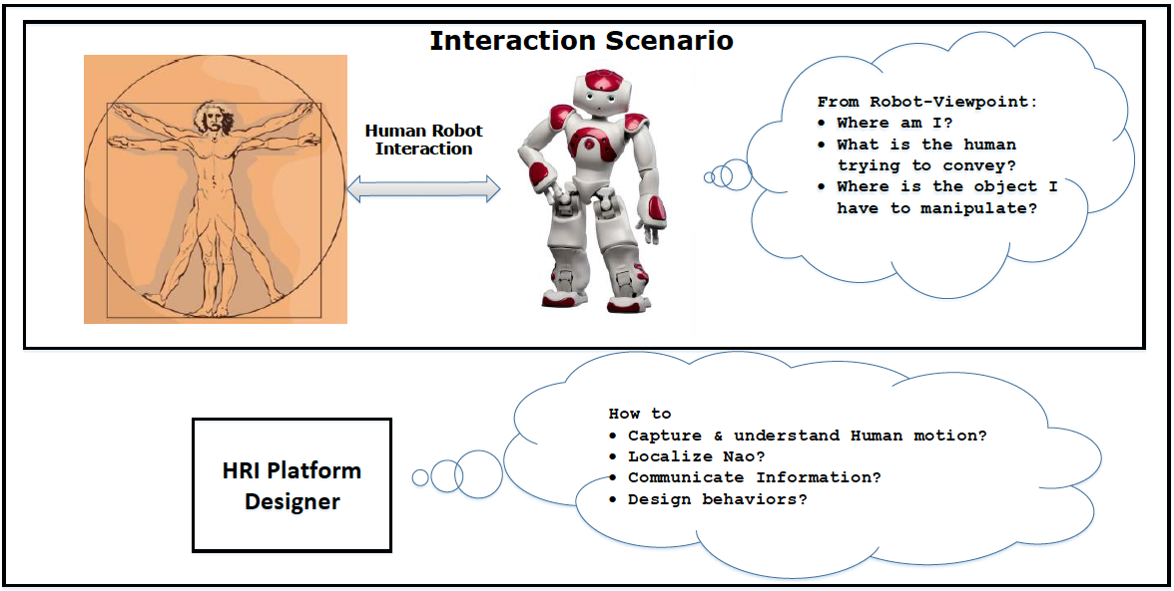
\includegraphics[width=\textwidth]{assets/ProblemStatement.pdf}
\caption{Concise depiction of Problem statement}
\label{fig:problemstatement}
\end{figure}% 

	This bibliographic study will summarize the state-of-the-art tools and techniques available in order to address each of the problem statements described above.

\section{Organization of the report}
	The report is organized as follows. This chapter (Chapter~\ref{Chapter1}) introduced the topic of human-robot interaction and the problem statements of this thesis. Chapter~\ref{Chapter2} will give an overview of the system components like the humanoid robot and the perception system. Chapter~\ref{Chapter3} will describe the state of the art techniques on human pose estimation and gesture recognition. Chapter~\ref{Chapter4} will describe various techniques to localize and track the humanoid robot. Chapter~\ref{Chapter5} will present a study on the available robot behavioral design frameworks. Following this Chapter~\ref{Chapter6} will describe HRI design and evaluation techniques. Finally Chapter~\ref{Chapter7} presents an initial proposal of the experimental platform and provides some concluding remarks.
% Chapter Template
\chapter{State of the art techniques}

\label{Chapter2} % Change X to a consecutive number; for referencing this chapter elsewhere, use \ref{ChapterX}

\lhead{Chapter 2. \emph{State of the art techniques}} % Change X to a consecutive number; this is for the header on each page - perhaps a shortened title
 Research in any field is a continuous process. It is meaningless to propose altogether new approaches ruling out the techniques proposed in the literature. Hence a careful study of the state-of-the-art techniques is necessary. It will give a clarity of the approaches that could be incorporated, improved or improvised in the research study of interest. The experimental platform that is being aimed in this thesis is largely an integration of various available techniques which makes literature review even more crucial. This chapter discusses the various methods and techniques proposed in the literature for addressing the problems described in Section~\ref{sec:problem_statement}.
\section{Humanoid Robot}
NAO \cite{NaoTheRobot} is a humanoid robot developed in the year 2006 by Albebaran Robotics, the company which has proved itself in the development of interactive social robots.
\begin{figure}[H]
\centering
\begin{subfigure}[b]{0.25\textwidth}
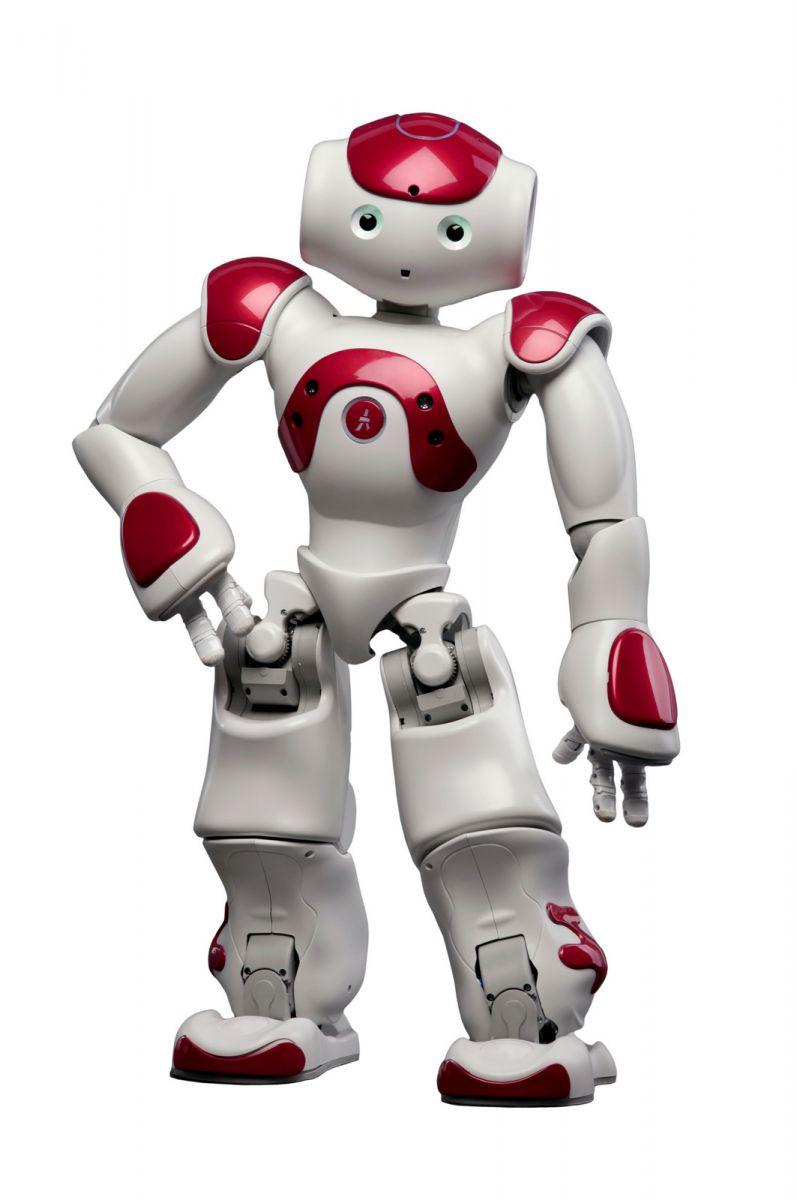
\includegraphics[width=\textwidth]{assets/nao_image1.jpg}
\caption{Robot appearance}
\label{fig:naojoint}
\end{subfigure}
\begin{subfigure}[b]{0.25\textwidth}
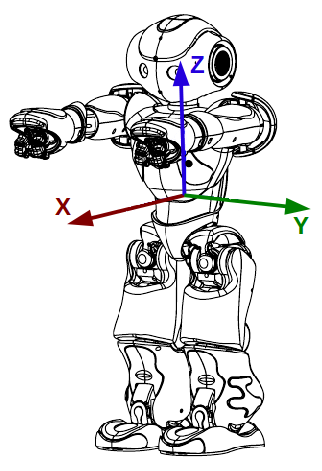
\includegraphics[width=\textwidth]{assets/hardware_inertialunit1.png}
\caption{Torso reference frame}
\label{fig:naoreference}
\end{subfigure}
\caption[NAO Humanoid Robot]{NAO Humanoid Robot. {Adopted from \cite{NaoTheRobot}}}
\label{fig:naorobot}
\end{figure}%
The intended scenarios include reception, assistance, home care, entertainment and even autism therapy. Nao has become a standard in academic world for research and education. In 2013, Aldebaran launched \emph{Autism Solution for Kids} \cite{ASKNao} initiative which offers a new teaching approach to teachers and children with autism. The technical specifications of the robot is shown in Fig~\ref{table:nao_spec}
\begin{table}[H]
\centering
\small
\caption{NAO humanoid platform technical specifications}
\label{table:nao_spec}
    \begin{tabular}{ | l | p{12cm} |}
    \hline
    \textbf{Category} & \textbf{Specification} \\
   \hline
  Version & NAO V50 H25 \\
                                          \hline
  Hardware & \begin{itemize}[leftmargin=*,topsep={0pt},itemsep={0pt},partopsep={0pt},parsep={0pt}] \item Body: 58 cm tall, 25 DOF composed of electric motors and actuators
  							\item Sensors: two cameras, four directional microphones, sonar rangefinder, two IR emitters and receivers, one inertial board, nine tactile sensors and eight pressure sensors
  							\item Communication devices: Voice synthesizer, LED lights, and 2 high-fidelity speakers
  							\item CPU: Intel ATOM 1.6ghz CPU 
  							\item Connectivity ; Ethernet and Wi-Fi
  							\item Power: 48.6-watt-hour battery that provides NAO with 1.5 or more hours of autonomy, depending on usage \end{itemize} \\
                                          \hline
                                          
  Motion  & \begin{itemize}[leftmargin=*,topsep={0pt},itemsep={0pt},partopsep={0pt},parsep={0pt}] \item Cartesian and Joint control. \item Omnidirectional walking, Whole body motion and Fall Manager \end{itemize} \\
                                          \hline
  
  Vision & \begin{itemize}[leftmargin=*,topsep={0pt},itemsep={0pt},partopsep={0pt},parsep={0pt}] \item Track, learn \& recognize images and faces. \item OpenCV support \end{itemize} \\
                                          \hline

  Audio & \begin{itemize}[leftmargin=*,topsep={0pt},itemsep={0pt},partopsep={0pt},parsep={0pt}] \item Sound Source Localization, Speech/Speaker recognition. \item Supports 19 languages.\end{itemize} \\
                                          \hline
  Software & \begin{itemize}[leftmargin=*,topsep={0pt},itemsep={0pt},partopsep={0pt},parsep={0pt}] \item OS: Linux kernel and supports NAOqi middleware
  							\item Tools: Choregraphe \cite{pot2009choregraphe} for designing behaviors
  							\item SDKs: C++/Python SDK for application developers \end{itemize} \\
                                          \hline
    \end{tabular}
\end{table}

\section{Human motion capture}
Human motion capture has been mainly developed to be used in medical, ergonomics, sports, robotics and other applications. Optical motion capture is one of the traditional ways of capturing the human motion (System like VICON$^{\regmark}$ have been deployed to aquire the \emph{MOCAP} data). However the main difficulty in the traditional optical motion capture system is the neccessity to equip the subject/actor with \emph{reflective markers}. The system itself is huge, expensive to setup and has to be calibrated before using. It suffers due to skin artifacts and not suitable for practical HRI scenarios. 
	
Other devices which are commonly used to capture the kinematic information are \emph{Accelerometers} and \emph{Inertial Measurement Unit(IMU)}. There are studies on understanding the human motion using IMU \cite{aoki2013segmentation} in which the human motion (arm only) is captured from IMU sensor and commercially available Wii$^{\regmark}$ remote. The complete understanding of the human motion requires lot of IMU sensors to be attached on the human body which will make the human motions more constrained. 

General-purpose robot perception usually relies on either traditional optical cameras or laser rangefinders, each having advantages and disadvantages. Cameras are fundamentally limited by the loss of 3-D structure in the 3-D or two-dimensional (2-D) projection and by their dependency on lighting conditions. The laser rangefinders allow much more robust sensing at long range but they are bulky and expensive.  

The RGB-D cameras combining the strengths of optical cameras and laser range finders enable a complete perception solution. RGB-D cameras\cite{ren2013change} are active sensors that provide high resolution dense color and depth information at real time frame rates. To reliably measure depth, RGB-D cameras use active sensing techniques, based on projected texture stereo, structured light, or time of flight. Unlike traditional stereo rigs, RGB-D sensors do not suffer calibration problems as both the projector and IR camera exhibit low distortion. The external correspondence between the camera and the projector is determined by a factory calibration. Moreover the rigid mount ensures that the devices do not have to be recalibrated during use.
\begin{figure}[H]
\centering
%\begin{subfigure}[b]{0.5\textwidth}
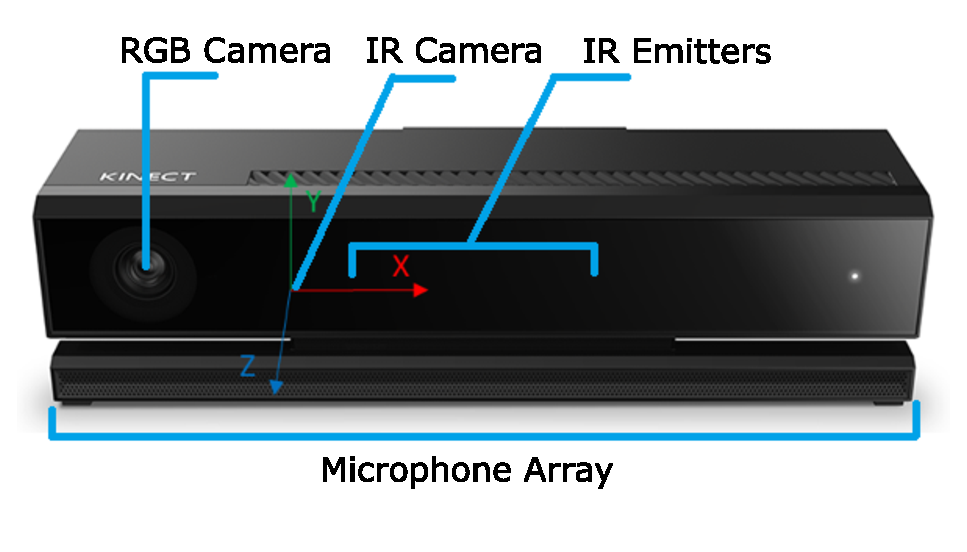
\includegraphics[width=0.5\textwidth]{assets/kinectv2_parts.eps}
%\caption{Kinect for Windows V2}
\label{fig:kinectv2}
%\end{subfigure}%
\caption[Kinect for Windows V2]{Kinect for Windows V2. {Adopted from manufacturer's site}}
%\label{fig:rgbd_sensors}
\end{figure}

A list of depth sensors available in the market along with their technical specification is shown in Table~\ref{table:rgbd_sensors} in Appendix~\ref{AppendixA}. Among them the Microsoft Kinect V2 \cite{Kinect2014} sensor has promising specifications and price. The Kinect comes with a powerful SDK \cite{KinectSDK2014} capable of performing skeleton tracking of upto 6 people (25 joints each) simultaneously out of the box. It also comes with the face detection, expression detection, gesture recognition and hand tracking. The Kinect studio software can record the sensor data and play back. It is also possible to build gestures and train the sensor to detect when it sees them later using the Visual gesture builder. 

\section{Human Motion Understanding} % Main chapter title
 Human motions are rich in information. It conveys to the receiver the emotion, the attitude, the deeds and even the health of the human. Without understanding completely the human motion, it is not possible to achieve a very good HRI system.  Vision based motion capture and analysis has been studied widely and a condensed summary of all the approaches developed during the past two decades until 2000 have been presented by Moeslund et al. in \cite{Moeslund2001231} followed by the study of advancements during the years 2000-2006 in the survey \cite{Moeslund200690}. Another work by Ronald Poppe \cite{Poppe20074} on the overview of vision based human motion analysis approached the problem into two discrete problems of modeling and estimation.
\subsection{Human Pose Estimation}
\label{sec:humanpose}
The surveys \cite{Moeslund2001231}\cite{Moeslund200690}\cite{Poppe20074} cited previously have investigated vision based human motion capture and analysis in general, however our particular focus is to use RGB-D sensors to this purpose. Human pose estimation has traditionally suffered from two main problems
\begin{itemize}
\item Necessary to adopt an initialization pose.
\item Losing track after a few frames.
\end{itemize}
So alternative techniques which do not require to adopt an initialization pose and estimate pose from single depth images is proposed by Shotton et al., \cite{shotton2013real} \cite{shotton2013efficient}. The studies propose two approaches shown in Figure~\ref{fig:kinect_pose} namely \emph{Body Part Classification (BPC)} and \emph{Offset Joint Regression (OJR)} for human pose estimation which are capable of accurately predicting the 3D positions of body joints using single depth images without using any temporal information. The two methods also share their use of a very large, realistic, synthetic training corpus, generated by rendering depth images of humans. The synthetic data is used to train deep random forests \cite{breiman2001random}, that can naturally handle a full range of human body shapes undergoing general body motions, self-occlusions, and poses cropped by the image frame. By using simple depth pixel comparison features, and parallelizable decision forests, both approaches could run in realtime on consumer hardware even without tracking a full body model. This is crucial in HRI because there are scenarios in which the human might be sitting and there will be lot of occlusions. The key point in these algorithms is that they do background subtraction before the actual processing.
\begin{figure}[H]
\centering
% \begin{subfigure}[b]{0.35\textwidth}
% 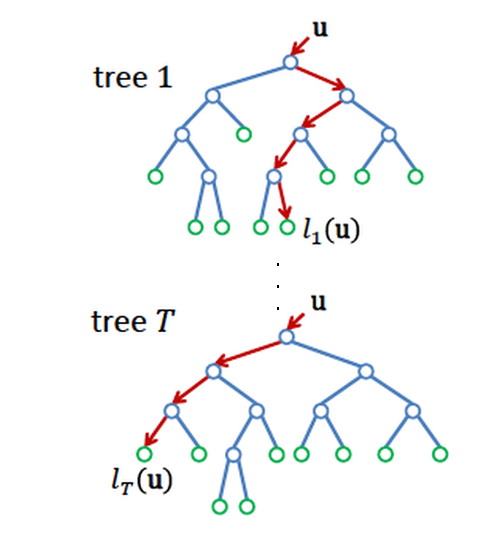
\includegraphics[width=\textwidth]{assets/forest.png}
% \caption{Randomized Decision Forests}
% \label{fig:decision_forests}
% \end{subfigure}
% \begin{subfigure}[b]{0.35\textwidth}
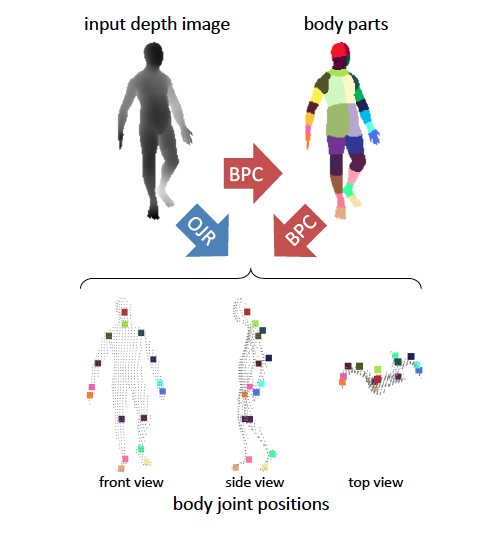
\includegraphics[width=0.4\textwidth]{assets/kinect_approaches.png}
% \caption{Human Pose estimation}
%\label{fig:kinect_pose}
%\end{subfigure}
\caption[Human pose estimation using single depth images]{Pose estimation using single depth images. {Adopted from \cite{shotton2013efficient}}}
\label{fig:kinect_pose}
\end{figure} 
% \subparagraph{Body Part Classification} % (fold)
% \label{subp:bpc} 
% The first approach employs an intermediate body parts representation, designed so that an accurate per-pixel classification of the parts will localize the joints of the body. It transforms the pose estimation problem into one that can be readily solved by classification algorithms. For the classification, \emph{31} body parts are defined: LU/RU/LW/RW head, neck, L/R shoulder, LU/RU/LW/RW arm, L/R elbow, L/R wrist, L/R hand, LU/RU/LW/RW torso, LU/RU/LW/RW leg, L/R knee, L/R ankle, and L/R foot (Left, Right, Upper, Lower). The classification forest used for Body Part Classification (BPC) uses a probability mass function(PMF) - $p_l(c)$ over body parts $c$ as the prediction model. The classification forest helps achieve the per-pixel classification by storing a distribution $p_l(c)$ over the discrete body parts $c$ at each leaf $l$. For a given input pixel $u$, the tree is descended to reach leaf $l = l(u)$ and the distribution $p_l(c)$ is retrieved. The distributions are averaged together for all trees in the forest to give the final classification as
% \begin{equation}
% p(c\vert \textbf{u}) = \frac{1}{T}\sum_{l\in L(\textbf{u})} p_l(c)
% \label{eqn:bpc_dist}
% \end{equation}
% Where $p_l(c)$ is PMF at the leaf node corresponding to body part $c$, $u$ is input pixel and $T$ is number of decision trees. The image space predictions are next re-projected into world space. The re-projection function is denoted as $x(u) = (x(u); y(u); z(u))^\text{T}$. Conveniently, the known $z(u)$ from the calibrated depth camera allows to compute $x(u)$ and $y(u)$ trivially. The body parts inherently lie on the surface of the body, thus a learned per-joint vector ${\zeta_j} = (0,0,\zeta_j)^\text{T}$ is used to push back the re-projected pixel surface positions into the world to better align with the interior joint position: $x_j(u) = x(u) + {\zeta_j}$. 
% \subparagraph{Offset Joint Regression} % (fold)
% \label{subp:ojr}  
% The second approach presented in \cite{shotton2013efficient} directly regresses the positions of body joints. The ground truth labels required for this approach are simply the ground truth 3D joint positions which are recorded during the mesh skinning process. In this approach \emph{16} body joints are defined: head, neck, L/R shoulder, L/R elbow, L/R wrist, L/R hand, L/R knee, L/R ankle, and L/R foot. The regression forest used for Offset Joint Regression (OJR) uses a set of weighted relative votes $V_{lj}$ for each joint $j$. At each leaf node $l$ a distribution over the relative 3D offset from the re-projected pixel coordinate $x(u)$ to each body joint $j$ of interest is stored. Each pixel can thus potentially cast votes to all joints in the body, and unlike BPC, these votes may differ in all world space coordinates and thus directly predict interior rather than surface positions. The distribution at the leaf node is represented using a \emph{small} set of 3D \emph{relative vote} vectors $\Delta_{ljk} \in \Re^3$. The subscript $l$ denotes the leaf node, $j$ denotes a body joint and $k \in \lbrace 1,...,K \rbrace$ denotes the maximum number of relative votes allowed. A confidence weight $w_{ljk}$ is associated with each vote and it is critical for the accuracy. The set of relative votes for joint $j$ at the node $l$ is denoted as $V_{lj}={{\lbrace (\Delta_{ljk},w_{ljk}) \rbrace}^K}_{k=1}$. In order to improve the speed, $N_{sub}$ samples could be obtained from ${X_j}^{OJR}$ by either random sampling or picking top $N_{sub}$ samples from it. 
%\subsubsection{Estimation using both Depth and RGB image}

Unlike the approaches used in the Kinect SDK, the approach presented in \cite{buys2014adaptable} uses both the depth and color (RGB-D) data for human body detection and pose estimation using a customizable human kinematic model. Other merits include the requirement of less training data and open source nature of this approach. This method makes use of iterative refinement technique in order to estimate the pose of multiple people among clutter and occlusion. The algorithm developed as part of this work has been implemented as part of the PCL \cite{rusu20113d} library under the name \emph{People's library}.
% \begin{figure}[H]
% \centering
% 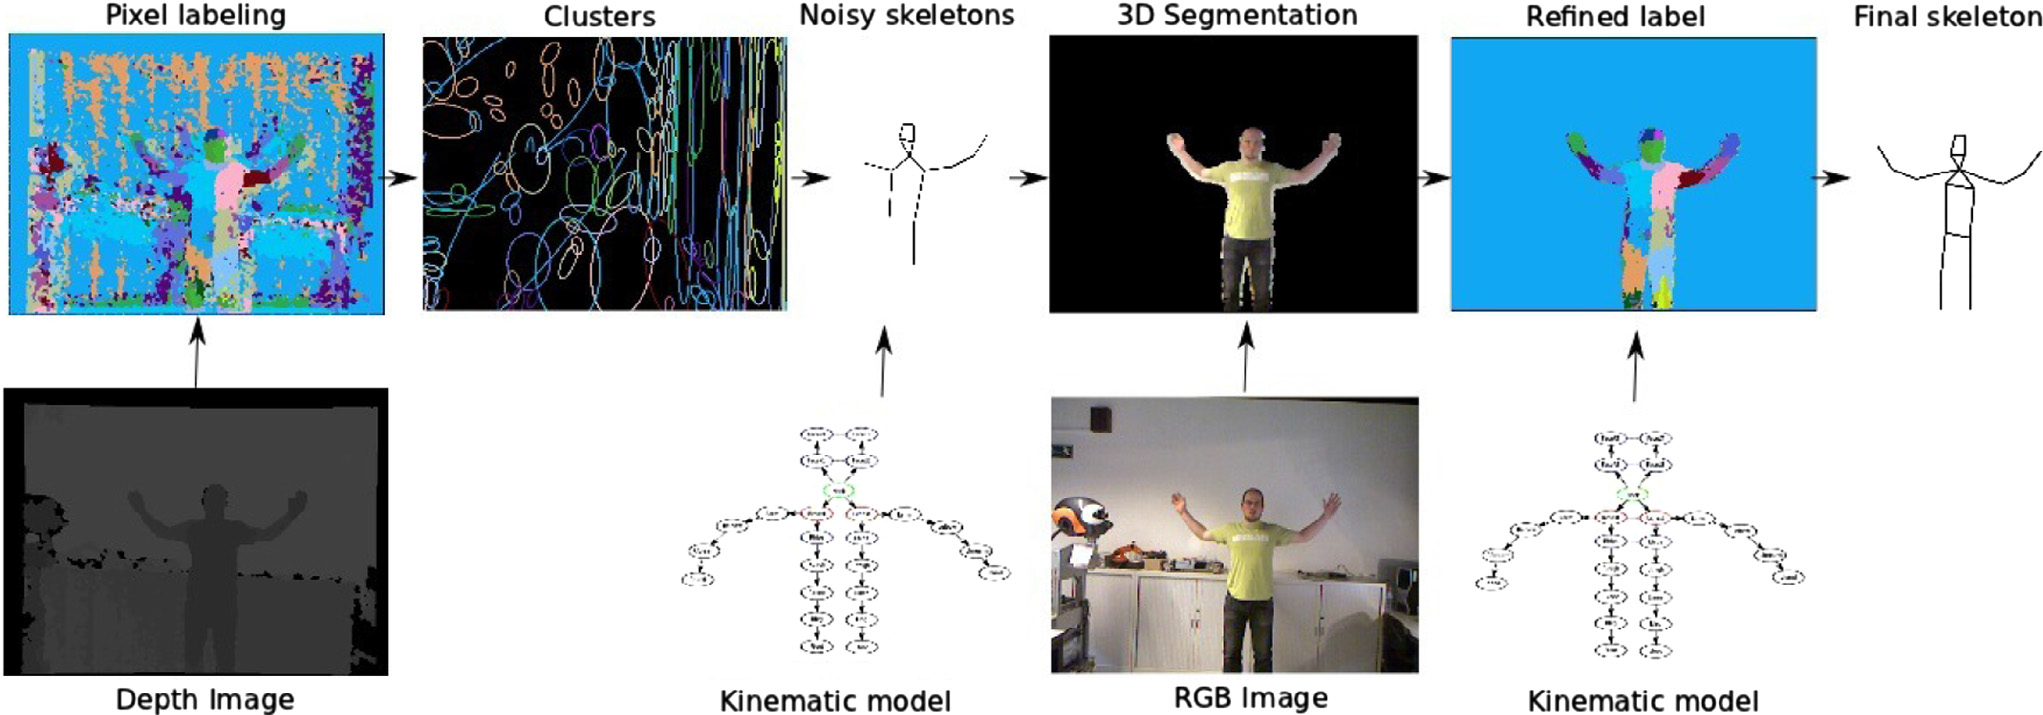
\includegraphics[width=\textwidth]{assets/adaptable_system_rgbd.png}
% \caption[Adaptable system for human body detection and pose estimation]{Adaptable system for human body detection \& pose estimation. {Adapted from \cite{buys2014adaptable}}}
% \label{fig:adaptable_rgbd}
% \end{figure}
% The goal of this approach is to output the 3D locations of the human body parts that are predefined in a kinematic model using the data received from an RGB-D sensor. The higher level process flow diagram of the system is shown in Figure~\ref{fig:adaptable_rgbd}. To start with, for a single depth map frame, per-pixel labeling is done using the similar approach described in \cite{shotton2013real}. However the principal difference is that no \emph{background subtraction} or fixed-pose initialization step before pixel labeling. A body part proposal step is performed on the initial noisy result, which results in a more robot part estimates. Using the statistical inference of the part estimates, a search for feasible kinematic trees is conducted during the kinematic tree search step. This result in the person detections and noisy skeletonization. In order to improve the obtained estimate, a second iteration of per-pixel body part labeling, body part proposal and kinematic tree search is performed. An appearance model is estimated online for segmentation refinement step. The noisy initial estimate obtained during the first iteration is used as a seed for color and depth-based segmentation that retrieves missing body parts and better localizes existing parts. This process can be used for multiple people among clutter and occlusion. This algorithm has been implemented as part of the PCL \cite{rusu20113d} library under the name \emph{People's library}.

\subsection{Human action recognition}
Understanding of human motion is not complete if the gesture of the human could not be understood. Hidden Markov models (HMM) which had been widely used for speech recognition \cite{rabiner1989tutorial} also inspired to be used for the gesture recognition applications. The HMM model is generated for each motion primitives and Viterbi algorithm is used to find the optimum sequence of the states given a set of observations. During the recognition step a likelihood function is used on the segmented motion pattern against each HMM and the motion primitive corresponding to HMM with large likelihood is selected.
% as shown in Figure~\ref{fig:hmm}. 
% Auto segmentation of arm motion and recognition of motion patterns using angular velocity data obtained by IMU sensors and the Wii remote using HMM has been demostrated in \cite{aoki2013segmentation}. 
% \begin{figure}[H]
% \centering
% 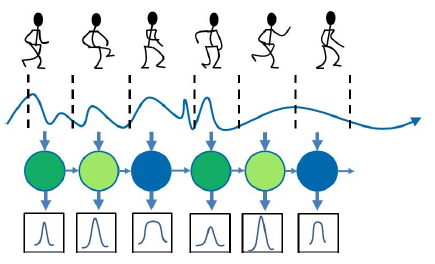
\includegraphics[width=0.3\textwidth]{assets/HMM.png}
% \caption[HMM motion modeling]{HMM motion modeling. {Adapted from \cite{aoki2013segmentation}}}
% \label{fig:hmm}
% \end{figure}
% In the publication by Microsoft research \cite{han2013enhanced}, a background study on various algortihms used for human activity analysis is presented. Recently \cite{KinectSDK2014} data-driven machine learning approaches like neural networks, Support vector machines, clustering, decision trees and bayesian networks are being exploited to this purpose. In \cite{KinectSDK2014}, an AdaBoost (Adaptive Boosting) algorithm \cite{freund1997decision} which is one of the top 10 data mining algorithms, is used to efficiently detect the gestures. The system involves a training phase in which the desired gestures are captured and tagged. These tagged gestures will be used by a gesture detector trainer which will generate a set of training examples $S=\lbrace \lbrace x_n,y_n \rbrace,\ n=1,\cdots,N \vert x_n\in X,y_n\in Y, X=\text{skeleton},Y=\lbrace -1,+1 \rbrace\rbrace$, associated data and set of weak classifiers $h_t$ and it learns the confidence $\alpha_t$ for $h_t$. The training results are stored in files and will be used by the gesture detector to perform per-frame classification of the data using $(h_t,\alpha_t)$. This approach has been proved to be robust with accuracy as high as 94.9\%. The gesture recognition module that comes with Kinect system already implements Adaboost based gesture detector for detecting the discrete gestures. For detecting more complex continuous gestures it uses RFRProgress detector, which is a detection technology that produces an analog or continuous result. It uses the Random Forest Regression (RFR) machine learning algorithm to determine the progress of a gesture performed by a user. It uses tagging models that are represented by analog signals that occur during a gesture. The RFRProgress is a context-based detector, meaning that the progress detection is only valid when a user is performing a gesture. Progress detection is enabled when a discrete gesture (AdaBoostTrigger) is detected.

In the publication by Microsoft research \cite{han2013enhanced}, a background study on various algortihms used for human activity analysis is presented. Recently \cite{KinectSDK2014} data-driven machine learning approaches like neural networks, Support vector machines, clustering, decision trees and bayesian networks are being exploited to this purpose. In \cite{KinectSDK2014}, an AdaBoost (Adaptive Boosting) algorithm \cite{freund1997decision} which is one of the top 10 data mining algorithms, is used to efficiently detect the gestures. The system involves a training phase in which the desired gestures are captured and tagged. These tagged gestures will be used by a gesture detector trainer which will generate a set of training examples, associated data and set of weak classifiers and it learns a confidence value for each of the weak classifiers. The training results are stored in files and will be used by the gesture detector to perform per-frame classification of the data. This approach has been proved to be robust with accuracy as high as 94.9\%. For detecting more complex continuous gestures it uses RFRProgress detector, which is a detection technology that produces an analog or continuous result. It uses the Random Forest Regression (RFR) machine learning algorithm to determine the progress of a gesture performed by a user. It uses tagging models that are represented by analog signals that occur during a gesture. The RFRProgress is a context-based detector, meaning that the progress detection is only valid when a user is performing a gesture. Progress detection is enabled when a discrete gesture (AdaBoostTrigger) is detected.

\section{Localization of Humanoid Robot} % Main chapter title
The localization of humanoid robots is a challenging issue, due to rough odometry estimation, noisy onboard sensing, and the swaying motion caused by walking \cite{cervera2012localization}. For most of the humanoid robots the reference frame will be fixed to the torso as is the case for the Nao. So the basic idea is to track the torso of the Nao or any other position with the known transformation from the torso. In this section different techniques that could be effectively used for localization and tracking of the humanoid robot are presented.

\subsection{Artificial Marker based approaches}
Tracking rectangular fiducial markers can be interesting if one could embed those markers on the humanoid robot. This is one of the simplest and cheapest solution in terms of the computational power as it uses simple image processing algorithms. ARToolKit \cite{kato1999marker} implements video tracking libraries which can calculate the real camera position and orientation relative to physical markers in real time. Before camera-based 6DOF tracking can be performed, the camera must be calibrated once as a pre-processing step. The perspective projection and the camera distortion parameters obtained during this step will be used later during the tracking initialization phase. The marker detection algorithms perform simple edge detection followed by a search for quadrangles of known dimension in the incoming image frame. The resulting sub-images are then checked against the set of known patterns. When a pattern is detected, ARToolKit uses the marker’s edges for a first, coarse pose detection. In the next step the rotation part of the estimated pose is refined iteratively using matrix fitting. The resulting pose matrix defines a transformation from the camera plane to a local coordinate system in the centre of the marker.
\begin{figure}[H]
\centering
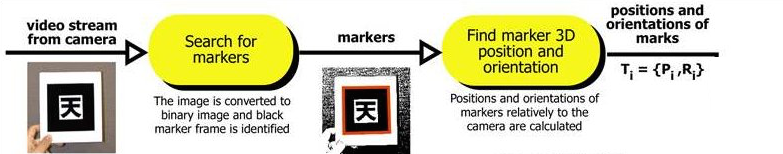
\includegraphics[width=1\textwidth]{assets/artoolkit.eps}
\caption[Marker tracking using ARToolKit]{Marker tracking using ARToolKit. {Adapted from \cite{kato1999marker}}}
\label{fig:artoolkit}
\end{figure}
\subsection{Point Cloud based approaches}
\label{ssec:pcl}
The Point Cloud Library (PCL) \cite{rusu20113d} which is one of the most widely used 3D perception software library, has collection of state-of-the-art algorithms and tools to process 3-D data. Point cloud library provides an excellent infrastructure for the object recognition and 6-DOF pose estimation pipeline by offering a wide variety of robust local and global features \cite{aldoma2012point}. 
% \begin{figure}[H]
% \centering
% 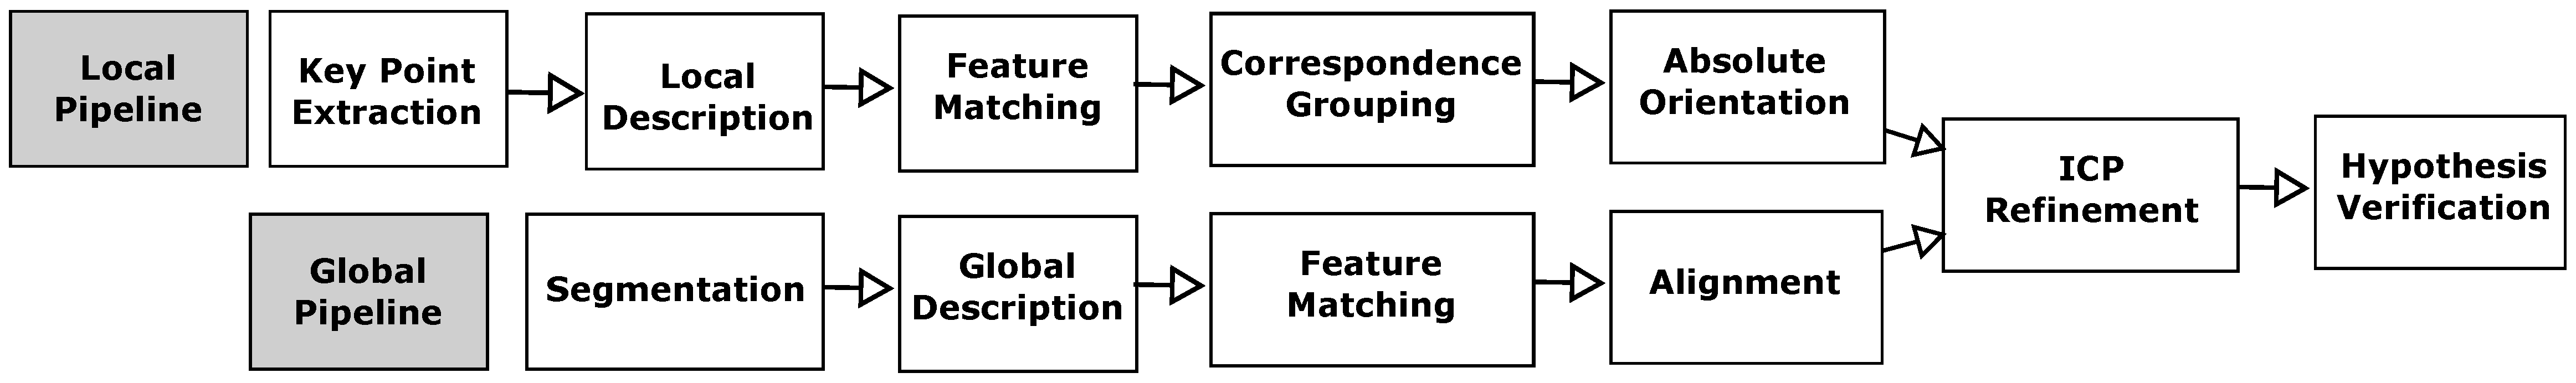
\includegraphics[width=1\textwidth]{assets/pcl_pipeline.eps}
% \caption[PCL local and global 3D Pipelines]{PCL local and global 3D Pipelines. {Adapted from \cite{aldoma2012point}}}
% \label{fig:pcl_pipeline}
% \end{figure}
The computation of pose of an object of known geometry requires the point clouds of the meshes to begin with. The 3D features known as descriptors of the model are computed and stored to be used during the recognition phase.  During the recognition, at first descriptors (local or global) of the incoming point cloud from sensor are computed followed by segmentation and correspondence matching with all the known models in the database. This is followed by an correspondence grouping using Random Sampling Consensus (RANSAC) to remove the outliers. Following this, a least square optimization is performed to obtain the rotation and the translation from exact point correspondences. Both the global and local pipelines can undergo an optional \emph{post processing} step by applying Iterated Closest Point (ICP) in order to refine estimated 6-DoF pose.

Apart from the object recognition and pose estimation pipeline, PCL provides a comprehensive algorithmic base for the tracking of 3D objects using Monte Carlo sampling techniques \cite{RUeda2012} and for calculating the likelihood using combined weighted metrics for hyperdimensional spaces including cartesian data, colors, and surface normals. PCL also has non-probabilistic tracking algorithms like Pyramidal Kanade Lucas Tomasi (KLT) Tracker in its tracking module. The KLT tracker operates on organized 3D keypoints with color/intensity information.
\subsection{Probabilistic approaches}
\label{ssec:prob_approaches}
Probabilistic localization algorithms are variants of the Bayes filter \cite{thrun2005probabilistic}. The pose of the robot is represented in a probabilistic manner called the \emph{belief}: ($bel(x_t)$) which is a posterior distribution over the state space. The basic principle behind Bayes filter is that the belief $bel(x_t)$ at time $t$ is calculated from the belief $bel(x_{t-1})$ at time $t-1$ along with the most recent control $u_t$ and the most recent measurement $z_t$. It involves two basic steps: \emph{Control update step} during which the $\overline{bel(x_t)}$ is computed based on the prior assigned to $x_{t-1}$ and the probability that control $u_t$ induces a transition from $x_{t-1}$ to $x_t$, \emph{Measurement update step} during which the hypothetical posterior $\overline{bel(x_t)}$ is multiplied with the probability of seeing an observation $z_t$ given this $x_t$. The recursive computation of belief state can thus be given by
\begin{align*}
\text{Control update step:}\quad \overline{bel(x_t)} &= \int p(x_t\vert u_t,x_{t-1})\cdot bel(x_{t-1}) dx \\
\text{Measurement update step:}\quad {bel(x_t)} &= \eta\cdot p(z_t\vert x_{t})\cdot \overline{bel(x_t)}
\end{align*}
where $\eta$ is the normalization factor. The Bayes filter forms the basis of Markov localization algorithms. Extended Kalman Filter(EKF) based localization is one of the initial developments to be used in non-linear state models. However they suffered problems of uni-modal distribution(gaussian) assumption and failing to solve global localization problem. The particle filter \cite{thrun2005probabilistic} is an alternative non-parametric implementation of bayes filter. The key idea of the particle filter is to represent the posterior $bel(x_t)$ by a set of samples drawn from the distribution. Such a representation is approximate, but it is nonparametric, and therefore can represent a much broader space of distributions than, for example, Gaussians. 
% The important steps of particle filter is sampling of the state space resulting in a set of $(M)$ particles, computing the importance factor $(w_t)$ of each of those particles $(x_t)$ based on strength of observation $(z_t)$ that could be observed from them and followed by re-sampling of the particles based on their importance factor. The basic intuition behind the particle filter is to approximate the belief $bel(x_t)$ by the set of particles $X_t$ and as a consequence denser a subregion of the state space is populated by samples, the more likely the true state falls in the region.The current state is given by the weighted particle mean 
% \begin{equation}
% E(X_t) = \sum_{m=1}^{M} {w_t}^{[m]}\cdot {x_t}^{[m]}
% \end{equation}
Monte-carlo localization (MCL) \cite{fox1999monte} is a version of Markov localization that uses fast sampling techniques to represent the belief and it introduces probabilistic motion and perceptual models into the particle filter framework. The efficiency of particle filters lies in the way they place computational resources. By sampling in proportion to likelihood, particle filters focus the computational resources on regions with high likelihood, where good approximations are most important. The time complexity of one update of the particle filter algorithm is linear in the number of samples needed for the estimation. 
%The Kullback-Leibler Distance(KLD) adaptive sampling technique proposed in \cite{fox2003adapting} presents an approach to adapt the number of samples over time. 
% \subsection{Existing Solutions}
% \label{sssec:prob_solutions}
	% \par The Point cloud library \cite{RUeda2012} introduced in Section~\ref{ssec:pcl} implements ready to use probabilistic tracking algorithms like: the most basic particle filter tracker(\emph{ParticleFilterTracker}), particle filter using OpenMP support(\emph{ParticleFilterOMPTracker}), KLD-adaptive sampling particle filter( \emph{KLDAdaptiveParticleFilterTracker}) and KLD adaptive sampling with OpenMP support ( \emph{KLDAdaptiveParticleFilterOMPTracker}). This could be readily used to track an object of know geometry and this information has to be fed to the PCL through a point cloud mesh of the object.
	
Studies on robot localization, obstacle mapping, and path planning in multilevel 3D environments by equipping Nao with a consumer-level depth camera have been reported in \cite{maier2012real}. This study provides real-time solution while maintaining a 3D environment representation and estimating the robot’s pose in 6D. The 3D environment model in form of an octree based representation containing the static parts of the environment is used. In this representation, the robot estimates its pose using MCL based on acquired depth data. Given the estimated 6D pose of the humanoid and a sequence of depth images, this approach continuously builds a local 3D representation of the current state of the environment containing also non-static obstacles. This learned octree-based representation is then used for real-time planning of collision-free paths. 
	
While \cite{maier2012real} presented an approach wherein a depth camera is fixed to the humanoid robot, in \cite{cervera2012localization} localization and motion planning in smart home environment have been proposed. In this study an external depth camera is used for 6D pose estimation and tracking, which is very close to the scenario of this thesis. Once again MCL technique is used for the pose estimation of the torso of the humanoid robot and this information is used for the closed loop navigation control. For the purpose of navigation, this study determined the pose error on the plane of walking using the knowledge of estimated pose and the desired pose. 
	
In \cite{choi2013rgb} a robust particle filter parallelized on a GPU that can track a known 3D object model over a sequence of RGB-D images is proposed. This method proposes to render the 3D object model to be used in the likelihood function so that the object could be tracked inspite of significant pose variations. Unlike PCL object tracking algorithm \cite{rusu20113d} which maintains only one reference point cloud, this approach uses multiple viewports rendered in GPU with different poses and each particle searches the closest rendering from the viewports and likelihood evaluation is performed by transforming the closest rendered result with the current particle state. This approach has been proved to be faster and also accurate than the PCL tracking. However the implementation of this algorithm is not open.
	
\section{Behavioral Frameworks} % Main chapter title
The users of social robots do not have necessary backgrounds in programming and design of robot behaviors. This lead to the development of several visual programming languages which allow non-programmers to create robot applications. Most of the available visual programming softwares allows to choose among many prebuilt behavioral blocks and connecting them to one another to get the desired flow of action \cite{MSRS4} \cite{Choregraphe}. These programs are very intuitive and allow the users to realize complex sequence of movements and sequential behaviors. But programming dynamic behaviors still remains challenging. This is primarily due to fact that the users have to think about the data flow between various blocks by appropriate connections between them. When it comes to designing complex dynamic behaviors this task becomes very tedious and time consuming. There are many solutions proposed in the literature that address the dynamic control problem. For instance Gostai's Universal Robotic Body Interface(URBI) \cite{baillie2008urbi} and Task description language (TDL) \cite{simmons1998task} are programming languages developed specifically for robot programming. URBI provides a modern object-oriented scripting language that allows the organization of code into different processes that either run sequentially or in parallel, and it also provides tools for process execution monitoring. In TDL which was developed as a C++ extension, the code is organized into task trees, which encode the hierarchical decomposition of tasks as well as the synchronization of constraints between tasks. More recently, specialized operating systems have been proposed, such as ROS \cite{quigley2009ros}, which organize code into distributed asynchronous modules that exchange data using a data subscription protocol. These solutions manage the integration and communication between different types of hardware and software and support the implementation of reaction, as well as behavioral specification. However, these programs have been produced by robot developers and are targeted at this community, which means that they are not intended to be used by non-roboticists and a solid background in computer science/robotics is required for their use.
% \begin{figure}[H]
% \centering
% \begin{subfigure}[b]{0.5\textwidth}
% 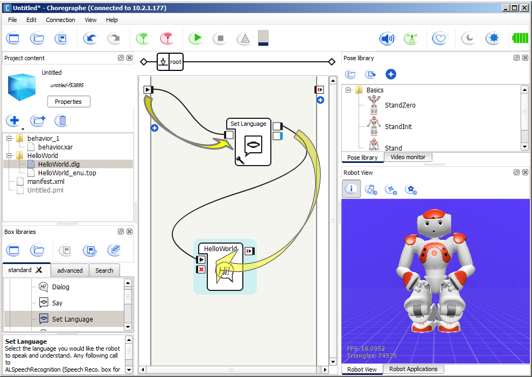
\includegraphics[width=\textwidth]{assets/helloworld_cho_dlg_05.png}
% %http://doc.aldebaran.com/2-1/getting_started/helloworld_choregraphe_dialog.html
% \caption{Choreographe Albebaran}
% \label{fig:choreographe}
% \end{subfigure}%
% \begin{subfigure}[b]{0.5\textwidth}
% 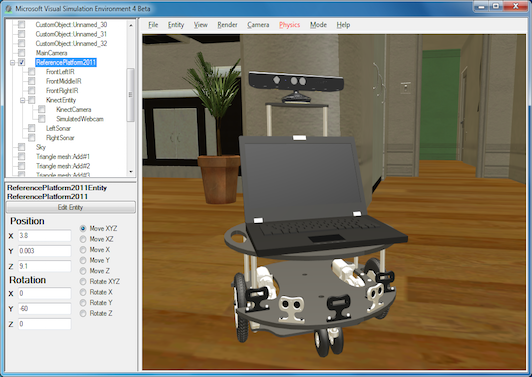
\includegraphics[width=\textwidth]{assets/MSRD4_VSE2.png}
% %http://www.microsoftstore.com/store/msusa/en_US/pdp/Kinect-for-Windows-v2-Sensor/productID.298810500
% \caption{MSRD Studio 4:Visual Simulation Environment}
% \label{fig:msrd4_vse}
% \end{subfigure}%
% \caption[Visual Programming Tools]{Visual Programming Tools. {Adapted from manufacturer's site}}
% \label{fig:visprog}
% \end{figure}
A non-domain-specific solution called \emph{Targets-Drives-Means (TDM)} is proposed in \cite{berenz2014targets} taking into account the aforementioned needs. TDM proposes a programming paradigm where temporal independent dynamic behaviors blocks run in parallel. The logic of the program is not expressed using communication links in a flowchart, but by the use of specialized dynamic components that regulate the activation status and the priorities of the behaviors. However there does not exist an intuitive interface for the behavior design yet and this framework is not open.
% \begin{figure}[H]
% \centering
% 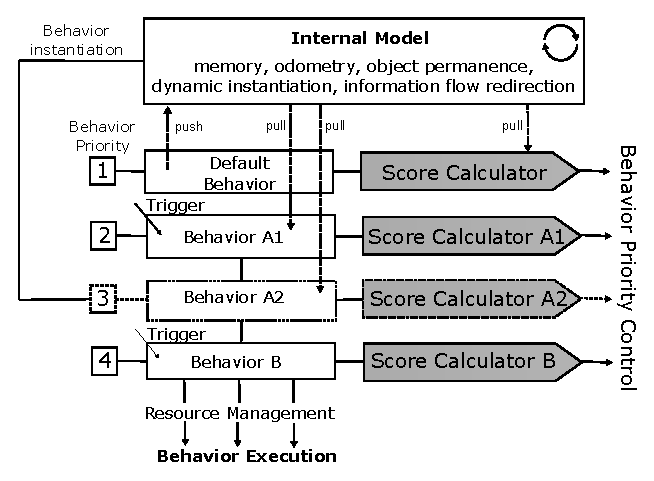
\includegraphics[width=0.5\textwidth]{assets/tdm_im.eps}
% \caption[Target-drives-means Framework]{TDM Framework. {Adapted from \cite{berenz2014targets}}}
% \label{fig:tdm_im}
% \end{figure}
\section{HRI Design and Evaluation} % Main chapter title
Human-Robot Interaction (HRI) being a rapidly advancing area of research, there is a growing need for strong experimental designs and methods of evaluation. This will bring credibility and validity to scientific research that involves humans as subjects, as recognized in the psychology and social science fields. As robots are becoming more prevalent, accurate methods to assess how humans respond to robots, how they feel about their interactions with robots, and how they interpret the actions of robots are very important. 

%\subparagraph{Planning, Design and Data collection}
A successful human study in HRI requires careful planning and design. In \cite{bethel2010review}, a set of questions when planning and designing a human study in HRI is presented. Apart from providing a checklist for planning and design of HRI studies, a list of recommendations for the experimental design and study execution is also provided in \cite{bethel2010review}.
	
Data collection is one of the important steps in the evaluation process. In \cite{Rogers2011} an insight of the design process of an interative system is presented. It discusses five key issues in the data gathering such as identifying participants, relationship with participants, setting goals, triangulation and importance of conducting pilot studies.
% \begin{itemize}
% \item \emph{Identifying participants} : Decide who to gather data from
% \item \emph{Relationship with participants} : Establishing a clear and professional relationship
% \item \emph{Setting goals} : Deciding how to analyze data once collected, Informed consent when appropriate
% \item \emph{Triangulation} : Looking at data from more than one perspective
% \item \emph{Pilot studies} : Small trial of main study. 
% \end{itemize}

An extensive review of HRI evaluation methods presented in \cite{bethel2010review} summarises five primary methods such as \emph{Self assessments}, \emph{Interviews}, \emph{Behavioral measures}, \emph{Psychophysiology measures} and \emph{Task performance metrics}. Each of these methods has advantages and disadvantages. However the study claims that it is possible to overcome these disadvantages by using three or more appropriate methods of evaluation. An effort to identify a set of common metrics to be used in task-oriented HRI can be found in \cite{Steinfeld2006}. This study proposes a set of metrics to evaluate the user, robot and the team (human-robot) performances.
%  the human-robot team and human-robot interactions and those proposed metrics are shown in Table~\ref{table:hri_metrics}
% \begin{table}[H]
% \centering
% \small
% \caption{Common metrics for task-based HRI}
% \label{table:hri_metrics}
% \begin{tabularx}{400pt}{c*3{X}}
% \toprule
%   \textbf{Common metrics} & \textbf{Sub-metrics} 
%                           & \textbf{Description}
%   \tabularnewline \midrule
  
%   \multirow{4}{*}{System Performance} & Quantitative performance & Assess the effectiveness and efficiency at performing a task. \\
%                                       & Subjective ratings & Assess the quality of the effort. \\
%                                       & Utilization of mixed-initiative & Ability of the human-robot team to appropriately regulate who has control initiative. 
%                                           \tabularnewline\midrule
                                          
%   \multirow{4}{*}{Operator Performance} & Situation Awareness (SA) & The degree to which the robot is situation aware. \\
%                                         & Workload & Relating human perceptions of cognitive load to operator SA \\
%                                         & Accuracy of mental models & Impact of Design affordances, operator expectations and stimulus-response compatibility.
%                                           \tabularnewline\midrule
  
%   \multirow{4}{*}{Robot Performance}  & Self Awareness & The degree to which a robot can accurately assess itself \\
%                                       & Human Awareness & The degree to which the robot is aware of humans \\
%                                       & Autonomy & The ability of robots to function independently without human intervention.
%                                           \tabularnewline                                
                                         
%   										\bottomrule
% \end{tabularx}
% \end{table}
Bartneck et al., \cite{bartneck2009measurement} emphasize the need for standardized measurement tools for human robot interaction. This work presents measurements tools in the form of questionnaires for five key concepts in HRI: anthropomorphism, animacy, likeability, perceived intelligence, and perceived safety. All the evaluation techniques rely on the statistical tools for validating the results and generalizing the phenomena. A summary of statistical tools for the data analysis in HRI can be found in Appendix~\ref{AppendixA}.


\section{Summary}

In this chapter a review of the literature which are most relevant to this thesis research is presented. The literature review helped to identify the appropriate techniques that could be used in the development of experimental platform. The key decisions made are shown in the Table~\ref{table:review_decisions}

\begin{table}[H]
\centering
\small
\caption{Identified techniques from state-of-the-art}
\label{table:review_decisions}
\begin{tabular}{ | l | p{10cm} |}
\hline
  \textbf{Problem to be addressed} & \textbf{Identified solution}
  \tabularnewline \hline
  
  Human motion understanding & The Kinect SDK \cite{KinectSDK2014} will suffice the human skeleton tracking. The Visual gesture builder tool that is shipped with Kinect SDK could be used for gesture creation and recogntion
                                          \tabularnewline\hline
                                          
  Localization of humanoid robot & The artificial marker based approaches seems to be the cheapest solution since we will be sharing the same sensor for motion recogntion as well. The ALVAR marker tracking library \cite{ALVAR} will be used to this purpose. 
                                          \tabularnewline\hline
  
  Application infrastructure & It has been decided to develop a \emph{proprietary application infrastructure} as existing solutions like ROS \cite{quigley2009ros} is not cross-platform and the Kinect sensor drivers for Linux are not mature enough at the time of this writing.
                                          \tabularnewline\hline

  Behavior framework & It has also been decided to develop a \emph{new behavior design and execution framework} as the existing solutions are not complete and they do not offer an end-to-end solution for naive users wanting to design HRI scenarios.
                                          \tabularnewline\hline

  HRI evaluation & The \emph{Self-assessment} techniques will be adopted and data collection will be done on a set of identified participants. Statistical analysis will be performed on the collected data.
                                          \tabularnewline\hline
\end{tabular}
\end{table} 
% Chapter Template
\chapter{State of the art techniques}

\label{Chapter3} % Change X to a consecutive number; for referencing this chapter elsewhere, use \ref{ChapterX}

\lhead{Chapter 3. \emph{State of the art techniques}} % Change X to a consecutive number; this is for the header on each page - perhaps a shortened title

  Research in any field is a continuous process. It is meaningless to propose altogether new approaches ruling out the techniques proposed in the literature. Hence a careful study of the state-of-the-art techniques is necessary. It will give a clarity of the approaches that could be incorporated, improved or improvised in the research study of interest. The experimental platform that is being aimed in this thesis is largely an integration of various available techniques which makes literature review even more crucial. This chapter discusses the various methods and techniques proposed in the literature for addressing the problems described in Section~\ref{sec:problem_statement}.

\section{Human Motion Understanding} % Main chapter title
 Human motions are rich in information. It conveys to the receiver the emotion, the attitude, the deeds and even the health of the human. Without understanding completely the human motion, it is not possible to achieve a very good HRI system.  Vision based motion capture and analysis has been studied widely and a condensed summary of all the approaches developed during the past two decades until 2000 have been presented by Moeslund et al. in \cite{Moeslund2001231} followed by the study of advancements during the years 2000-2006 in the survey \cite{Moeslund200690}. In the former the authors reviewed more than 130 publications while in the latter a review of over 300 publications was presented. This shows the rapid advancements in the study of the human motion in the recent times. Another work by Ronald Poppe \cite{Poppe20074} on the overview of vision based human motion analysis approached the problem into two discrete problems of modeling and estimation while also discussing the model free approaches to motion analysis. In this section an overview of the various approaches for pose estimation from RGB-D data and the gesture recognition are covered.
\subsection{Human Pose Estimation}
\label{sec:humanpose}
The surveys \cite{Moeslund2001231}\cite{Moeslund200690}\cite{Poppe20074} cited previously have investigated vision based human motion capture and analysis in general, however our particular focus is to use RGB-D sensors (presented in Section~\ref{ssec:rgbd_sensors}) to this purpose. Human pose estimation has traditionally suffered from two main problems
\begin{itemize}
\item Necessary to adopt an initialization pose.
\item Losing track after a few frames.
\end{itemize}
So alternative techniques which do not require to adopt an initialization pose and estimate pose from single depth images first appeared in the works of Shotton et al., \cite{shotton2013real}.
\subsubsection{Estimation from Single Depth Images}
 The initial publication by the Xbox team \cite{Kinect2014} appeared in \cite{shotton2013real} where real time human pose estimation in parts using single depth images has been proposed. An extension of this work has been published recently by the Microsoft computer vision research group \cite{shotton2013efficient}. This study proposes two approaches namely \emph{Body Part Classification (BPC)} and \emph{Offset Joint Regression (OJR)} for human pose estimation which are capable of accurately predicting the 3D positions of body joints using single depth images without using any temporal information. The two methods also share their use of a very large, realistic, synthetic training corpus, generated by rendering depth images of humans. Each render is assigned randomly sampled parameters including body shape, size, pose, scene position, etc., thus generating quickly and cheaply hundreds of thousands of varied images with associated ground-truth (the body part label images and the set of 3D body joint positions). This enables to train deep random forests \cite{breiman2001random}, without the risk of overfitting, that can naturally handle a full range of human body shapes undergoing general body motions, self-occlusions, and poses cropped by the image frame. By using simple depth pixel comparison features, and parallelizable decision forests, both approaches could run in realtime on consumer hardware. The per-frame, per-joint proposals described in this study have been demonstrated to be usable even without tracking a full body model. This is crucial in HRI because there are scenarios in which the human might be sitting and there will be lot of occlusions. The key point in these algorithms is that they do background subtraction before the actual processing 
\begin{figure}[H]
\centering
\begin{subfigure}[b]{0.35\textwidth}
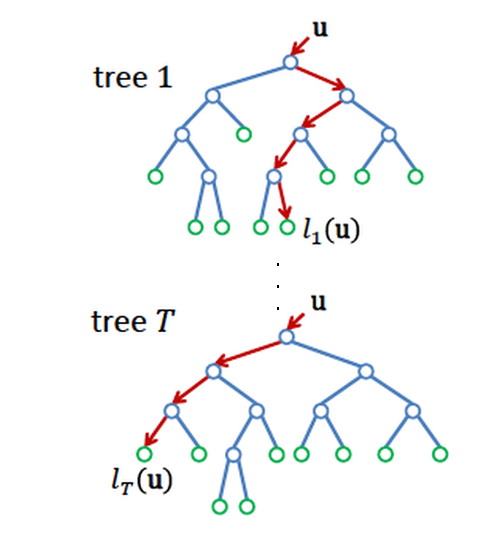
\includegraphics[width=\textwidth]{assets/forest.png}
\caption{Randomized Decision Forests}
\label{fig:decision_forests}
\end{subfigure}
\begin{subfigure}[b]{0.35\textwidth}
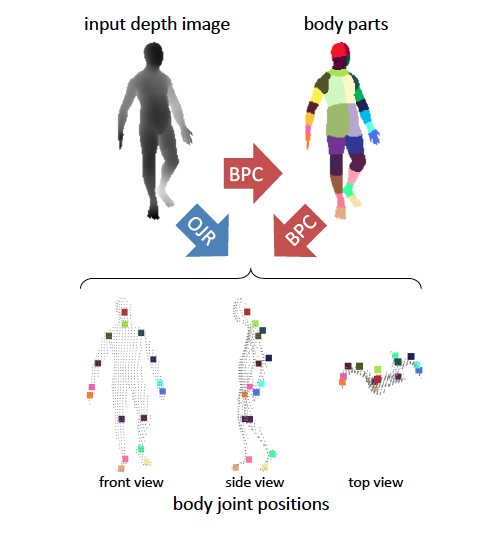
\includegraphics[width=\textwidth]{assets/kinect_approaches.png}
\caption{Human Pose estimation}
\label{fig:kinect_pose}
\end{subfigure}
\caption[Human pose estimation using single depth images]{Pose estimation using single depth images. {Adopted from \cite{shotton2013efficient}}}
\end{figure} 
% \subparagraph{Body Part Classification} % (fold)
% \label{subp:bpc} 
% The first approach employs an intermediate body parts representation, designed so that an accurate per-pixel classification of the parts will localize the joints of the body. It transforms the pose estimation problem into one that can be readily solved by classification algorithms. For the classification, \emph{31} body parts are defined: LU/RU/LW/RW head, neck, L/R shoulder, LU/RU/LW/RW arm, L/R elbow, L/R wrist, L/R hand, LU/RU/LW/RW torso, LU/RU/LW/RW leg, L/R knee, L/R ankle, and L/R foot (Left, Right, Upper, Lower). The classification forest used for Body Part Classification (BPC) uses a probability mass function(PMF) - $p_l(c)$ over body parts $c$ as the prediction model. The classification forest helps achieve the per-pixel classification by storing a distribution $p_l(c)$ over the discrete body parts $c$ at each leaf $l$. For a given input pixel $u$, the tree is descended to reach leaf $l = l(u)$ and the distribution $p_l(c)$ is retrieved. The distributions are averaged together for all trees in the forest to give the final classification as
% \begin{equation}
% p(c\vert \textbf{u}) = \frac{1}{T}\sum_{l\in L(\textbf{u})} p_l(c)
% \label{eqn:bpc_dist}
% \end{equation}
% Where $p_l(c)$ is PMF at the leaf node corresponding to body part $c$, $u$ is input pixel and $T$ is number of decision trees. The image space predictions are next re-projected into world space. The re-projection function is denoted as $x(u) = (x(u); y(u); z(u))^\text{T}$. Conveniently, the known $z(u)$ from the calibrated depth camera allows to compute $x(u)$ and $y(u)$ trivially. The body parts inherently lie on the surface of the body, thus a learned per-joint vector ${\zeta_j} = (0,0,\zeta_j)^\text{T}$ is used to push back the re-projected pixel surface positions into the world to better align with the interior joint position: $x_j(u) = x(u) + {\zeta_j}$. 
% \subparagraph{Offset Joint Regression} % (fold)
% \label{subp:ojr}  
% The second approach presented in \cite{shotton2013efficient} directly regresses the positions of body joints. The ground truth labels required for this approach are simply the ground truth 3D joint positions which are recorded during the mesh skinning process. In this approach \emph{16} body joints are defined: head, neck, L/R shoulder, L/R elbow, L/R wrist, L/R hand, L/R knee, L/R ankle, and L/R foot. The regression forest used for Offset Joint Regression (OJR) uses a set of weighted relative votes $V_{lj}$ for each joint $j$. At each leaf node $l$ a distribution over the relative 3D offset from the re-projected pixel coordinate $x(u)$ to each body joint $j$ of interest is stored. Each pixel can thus potentially cast votes to all joints in the body, and unlike BPC, these votes may differ in all world space coordinates and thus directly predict interior rather than surface positions. The distribution at the leaf node is represented using a \emph{small} set of 3D \emph{relative vote} vectors $\Delta_{ljk} \in \Re^3$. The subscript $l$ denotes the leaf node, $j$ denotes a body joint and $k \in \lbrace 1,...,K \rbrace$ denotes the maximum number of relative votes allowed. A confidence weight $w_{ljk}$ is associated with each vote and it is critical for the accuracy. The set of relative votes for joint $j$ at the node $l$ is denoted as $V_{lj}={{\lbrace (\Delta_{ljk},w_{ljk}) \rbrace}^K}_{k=1}$. In order to improve the speed, $N_{sub}$ samples could be obtained from ${X_j}^{OJR}$ by either random sampling or picking top $N_{sub}$ samples from it. 
\subsubsection{Estimation using both Depth and RGB image}
Unlike the approaches used in the Kinect SDK, the approach presented in \cite{buys2014adaptable} uses both the depth and color (RGB-D) data for human body detection and pose estimation using a customizable human kinematic model. Other merits include the requirement of less training data and open source nature of this approach. 
\begin{figure}[H]
\centering
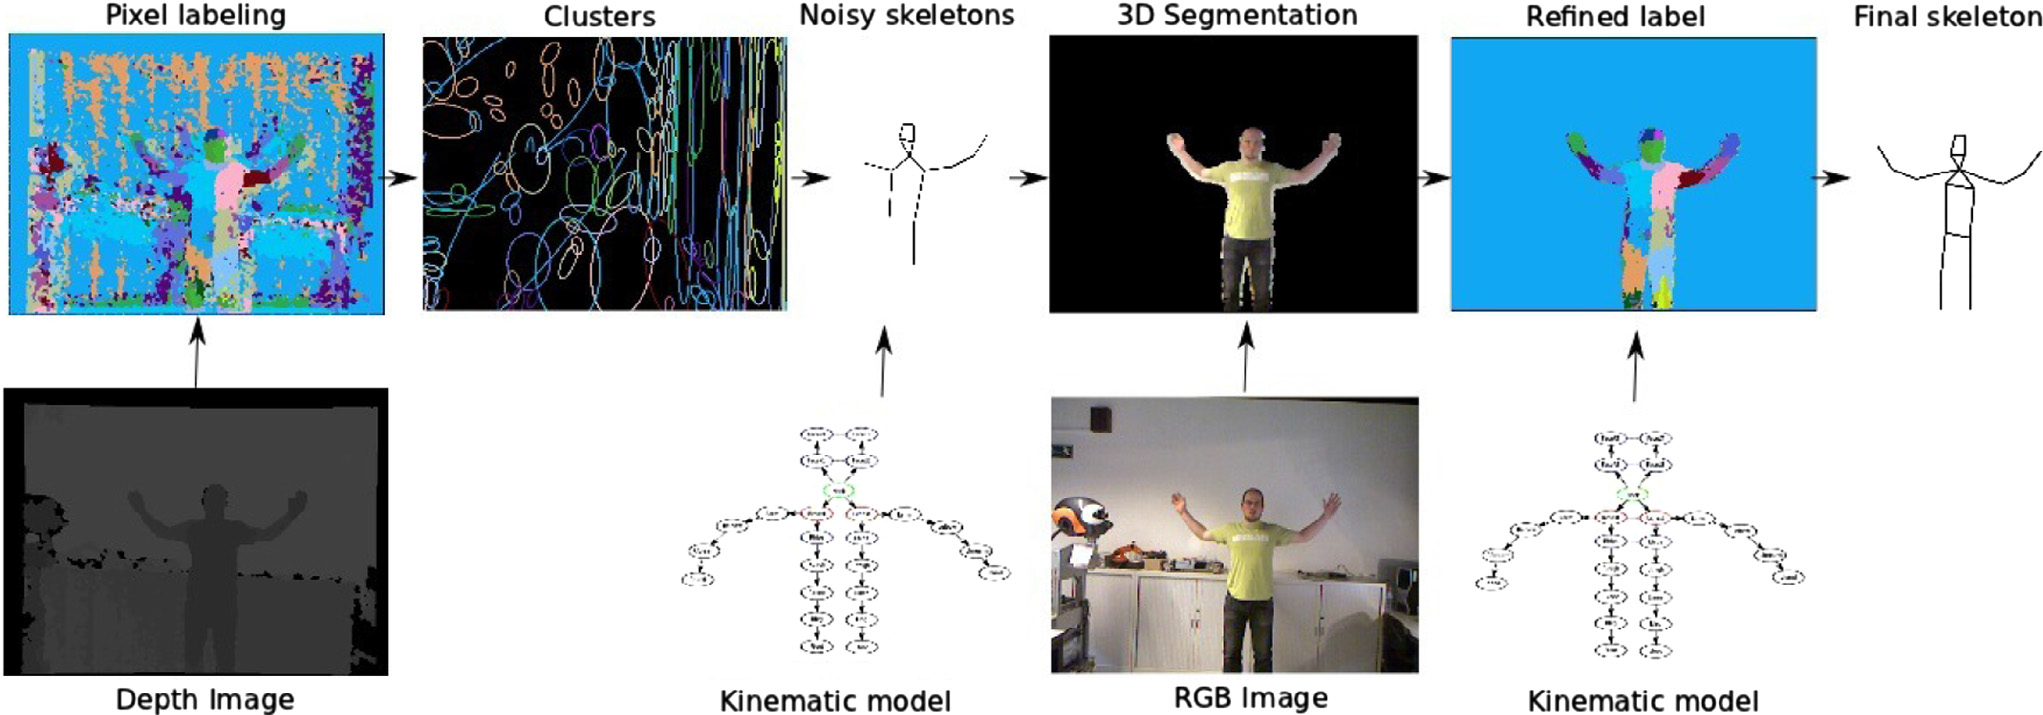
\includegraphics[width=\textwidth]{assets/adaptable_system_rgbd.png}
\caption[Adaptable system for human body detection and pose estimation]{Adaptable system for human body detection \& pose estimation. {Adapted from \cite{buys2014adaptable}}}
\label{fig:adaptable_rgbd}
\end{figure}
The goal of this approach is to output the 3D locations of the human body parts that are predefined in a kinematic model using the data received from an RGB-D sensor. The higher level process flow diagram of the system is shown in Figure~\ref{fig:adaptable_rgbd}. To start with, for a single depth map frame, per-pixel labeling is done using the similar approach described in \cite{shotton2013real}. However the principal difference is that no \emph{background subtraction} or fixed-pose initialization step before pixel labeling. A body part proposal step is performed on the initial noisy result, which results in a more robot part estimates. Using the statistical inference of the part estimates, a search for feasible kinematic trees is conducted during the kinematic tree search step. This result in the person detections and noisy skeletonization. In order to improve the obtained estimate, a second iteration of per-pixel body part labeling, body part proposal and kinematic tree search is performed. An appearance model is estimated online for segmentation refinement step. The noisy initial estimate obtained during the first iteration is used as a seed for color and depth-based segmentation that retrieves missing body parts and better localizes existing parts. This process can be used for multiple people among clutter and occlusion. This algorithm has been implemented as part of the PCL \cite{rusu20113d} library under the name \emph{People's library}.

\subsection{Gesture Recognition}
	Understanding of human motion is not complete if the gesture of the human could not be understood. The next step after the human pose is tracked is to recognise the gesture. Hidden Markov models (HMM) which had been widely used for speech recognition \cite{rabiner1989tutorial} also inspired to be used for the gesture recognition applications. The HMM model is generated for each motion primitives and Viterbi algorithm is used to find the optimum sequence of the states given a set of observations. During the recognition step a likelihood function is used on the segmented motion pattern against each HMM and the motion primitive corresponding to HMM with large likelihood is selected as shown in Figure~\ref{fig:hmm}. Auto segmentation of arm motion and recognition of motion patterns using angular velocity data obtained by IMU sensors and the Wii remote using HMM has been demostrated in \cite{aoki2013segmentation}. 
\begin{figure}[H]
\centering
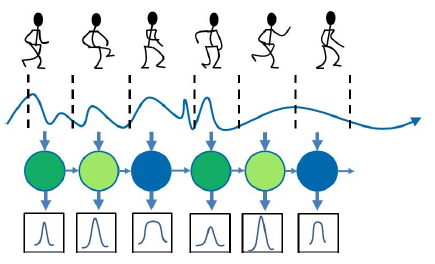
\includegraphics[width=0.3\textwidth]{assets/HMM.png}
\caption[HMM motion modeling]{HMM motion modeling. {Adapted from \cite{aoki2013segmentation}}}
\label{fig:hmm}
\end{figure}
% In the publication by Microsoft research \cite{han2013enhanced}, a background study on various algortihms used for human activity analysis is presented. Recently \cite{KinectSDK2014} data-driven machine learning approaches like neural networks, Support vector machines, clustering, decision trees and bayesian networks are being exploited to this purpose. In \cite{KinectSDK2014}, an AdaBoost (Adaptive Boosting) algorithm \cite{freund1997decision} which is one of the top 10 data mining algorithms, is used to efficiently detect the gestures. The system involves a training phase in which the desired gestures are captured and tagged. These tagged gestures will be used by a gesture detector trainer which will generate a set of training examples $S=\lbrace \lbrace x_n,y_n \rbrace,\ n=1,\cdots,N \vert x_n\in X,y_n\in Y, X=\text{skeleton},Y=\lbrace -1,+1 \rbrace\rbrace$, associated data and set of weak classifiers $h_t$ and it learns the confidence $\alpha_t$ for $h_t$. The training results are stored in files and will be used by the gesture detector to perform per-frame classification of the data using $(h_t,\alpha_t)$. This approach has been proved to be robust with accuracy as high as 94.9\%. The gesture recognition module that comes with Kinect system already implements Adaboost based gesture detector for detecting the discrete gestures. For detecting more complex continuous gestures it uses RFRProgress detector, which is a detection technology that produces an analog or continuous result. It uses the Random Forest Regression (RFR) machine learning algorithm to determine the progress of a gesture performed by a user. It uses tagging models that are represented by analog signals that occur during a gesture. The RFRProgress is a context-based detector, meaning that the progress detection is only valid when a user is performing a gesture. Progress detection is enabled when a discrete gesture (AdaBoostTrigger) is detected.
In the publication by Microsoft research \cite{han2013enhanced}, a background study on various algortihms used for human activity analysis is presented. Recently \cite{KinectSDK2014} data-driven machine learning approaches like neural networks, Support vector machines, clustering, decision trees and bayesian networks are being exploited to this purpose. In \cite{KinectSDK2014}, an AdaBoost (Adaptive Boosting) algorithm \cite{freund1997decision} which is one of the top 10 data mining algorithms, is used to efficiently detect the gestures. The system involves a training phase in which the desired gestures are captured and tagged. These tagged gestures will be used by a gesture detector trainer which will generate a set of training examples, associated data and set of weak classifiers and it learns a confidence value for each of the weak classifiers. The training results are stored in files and will be used by the gesture detector to perform per-frame classification of the data. This approach has been proved to be robust with accuracy as high as 94.9\%. The gesture recognition module that comes with Kinect system already implements Adaboost based gesture detector for detecting the discrete gestures. For detecting more complex continuous gestures it uses RFRProgress detector, which is a detection technology that produces an analog or continuous result. It uses the Random Forest Regression (RFR) machine learning algorithm to determine the progress of a gesture performed by a user. It uses tagging models that are represented by analog signals that occur during a gesture. The RFRProgress is a context-based detector, meaning that the progress detection is only valid when a user is performing a gesture. Progress detection is enabled when a discrete gesture (AdaBoostTrigger) is detected.

\section{Localization of Humanoid Robot} % Main chapter title
The localization of humanoid robots is a challenging issue, due to rough odometry estimation, noisy onboard sensing, and the swaying motion caused by walking \cite{cervera2012localization}. As a prelimnary assumption, the link of the robot are considered \emph{rigid bodies} in which distance between any two given points on it remains constant in time regardless of external forces exerted on it. Rigid body transformation forms the basic components in the pose estimation framework. In the $3D$ operational space represented by the vector space $\Re^3$, a rigid body is represented by \emph{6 degrees of freedom (DOF)}, 3 for the position along each of the coordinate axes (cartesian coordinates) $P = [p_x,p_y,p_z]^{\text{T}}$ and 3 for the orientation $R$. There are different representation for the orientation of the rigid body. They are rotation matrices, euler angles, RPY (roll,pitch,yaw) angles, quaternions. A detailed introduction about rigid body mechanics and various representation of pose of a rigid body can be found in the book by Khalil et al., \cite{khalil2004modeling}. For most of the humanoid robots the reference frame will be fixed to the torso as is the case for the Nao. So the basic idea is to track the torso of the Nao or any other position with the known transformation from the torso. In this section different techniques that could be effectively used for localization and tracking of the humanoid robot are presented.

\subsection{Artificial Marker based approaches}
The advancements in the field of augmented reality led to the development of efficient tracking of object poses by employing fiducial markers. Tracking rectangular fiducial markers can be interesting if we could embed those markers on the humanoid robot. This is one of the simplest and cheapest solution in terms of the computational power as it uses simple image processing algorithms. ARToolKit \cite{kato1999marker} implements video tracking libraries which can calculate the real camera position and orientation relative to physical markers in real time. Before camera-based 6DOF tracking can be performed, the camera must be calibrated once as a pre-processing step. The perspective projection and the camera distortion parameters obtained during this step will be used later during the tracking initialization phase. During the tracking, as a first step ARToolKit performs a very simple edge detection by thresholding the complete image with a constant value, followed by a search for quadrangles. Resulting areas being either too large or too small are immediately rejected. Next the interior areas of the remaining quadrangles are normalized using a perspective transformation. The resulting sub-images are then checked against the set of known patterns. When a pattern is detected, ARToolKit uses the marker’s edges for a first, coarse pose detection. In the next step the rotation part of the estimated pose is refined iteratively using matrix fitting. The resulting pose matrix defines a transformation from the camera plane to a local coordinate system in the centre of the marker.
\begin{figure}[H]
\centering
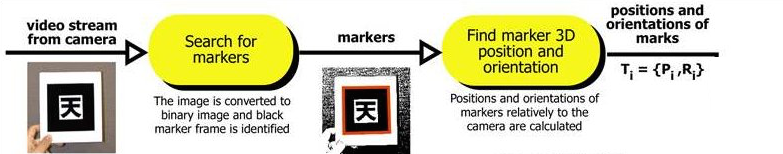
\includegraphics[width=1\textwidth]{assets/artoolkit.eps}
\caption[Marker tracking using ARToolKit]{Marker tracking using ARToolKit. {Adapted from \cite{kato1999marker}}}
\label{fig:artoolkit}
\end{figure}
\subsection{Point Cloud based approaches}
\label{ssec:pcl}
The Point Cloud Library (PCL) \cite{rusu20113d} which is one of the most widely used 3D perception software library, has collection of state-of-the-art algorithms and tools to process 3-D data. 
	Point cloud library provides an excellent infrastructure for the object recognition and 6-DOF pose estimation pipeline by offering a wide variety of robust local and global features. A list of features available is presented in \cite{aldoma2012point}. Object recognition based on global/local features almost share the same flow of operations. 
% \begin{figure}[H]
% \centering
% 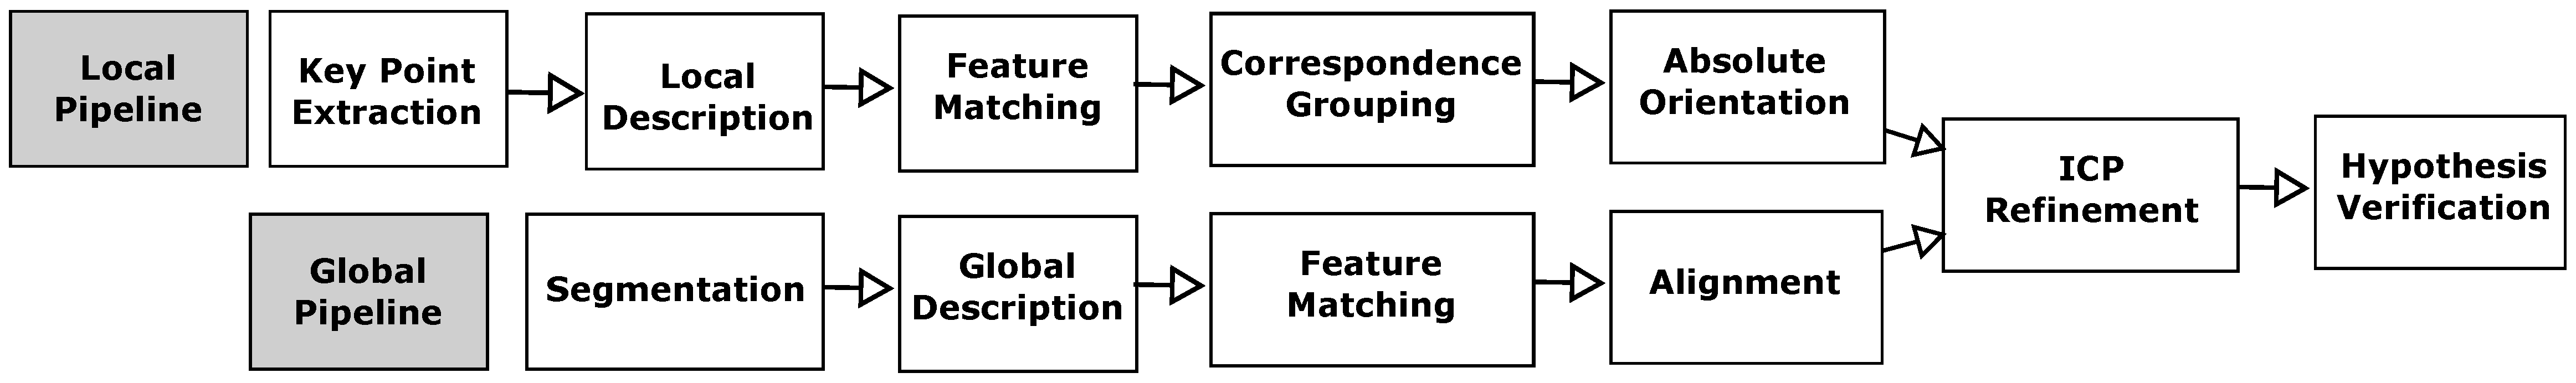
\includegraphics[width=1\textwidth]{assets/pcl_pipeline.eps}
% \caption[PCL local and global 3D Pipelines]{PCL local and global 3D Pipelines. {Adapted from \cite{aldoma2012point}}}
% \label{fig:pcl_pipeline}
% \end{figure}
The pose of an object of known geometry is computed with the point clouds of the meshes generated by a virtual depth camera. The 3D features known as descriptors of the model are computed and stored to be used during the recognition phase.  During the recognition, at first descriptors (local or global) are computed followed by segmentation and correspondence matching with all the known models in the database. This is followed by an correspondence grouping using Random Sampling Consensus (RANSAC) to remove the outliers. Following this, a least square optimization is performed to obtain the rotation and the translation from exact point correspondences. Both the global and local pipelines can undergo an optional \emph{post processing} step by applying Iterated Closest Point (ICP) in order to refine estimated 6-DoF pose.

Apart from the object recognition and pose estimation pipeline, PCL provides a comprehensive algorithmic base for the tracking of 3D objects using Monte Carlo sampling techniques \cite{RUeda2012} and for calculating the likelihood using combined weighted metrics for hyperdimensional spaces including cartesian data, colors, and surface normals. PCL also has non-probabilistic tracking algorithms like Pyramidal Kanade Lucas Tomasi (KLT) Tracker in its tracking module. The KLT tracker operates on organized 3D keypoints with color/intensity information. A list of probabilistic tracking algorithms implemented in PCL is presented in Section~\ref{sssec:prob_solutions} for the purpose of being coherent.
\subsection{Probabilistic approaches}
\label{ssec:prob_approaches}
Probabilistic localization algorithms are variants of the Bayes filter \cite{thrun2005probabilistic}. The pose of the robot is represented in a probabilistic manner called the \emph{belief}: ($bel(x_t)$) which is a posterior distribution over the state space. The basic principle behind Bayes filter is that the belief $bel(x_t)$ at time $t$ is calculated from the belief $bel(x_{t-1})$ at time $t-1$ along with the most recent control $u_t$ and the most recent measurement $z_t$. It involves two basic steps: \emph{Control update step} during which the $\overline{bel(x_t)}$ is computed based on the prior assigned to $x_{t-1}$ and the probability that control $u_t$ induces a transition from $x_{t-1}$ to $x_t$, \emph{Measurement update step} during which the hypothetical posterior $\overline{bel(x_t)}$ is multiplied with the probability of seeing an observation $z_t$ given this $x_t$. The recursive computation of belief state can thus be given by
\begin{align*}
\text{Control update step:}\quad \overline{bel(x_t)} &= \int p(x_t\vert u_t,x_{t-1})\cdot bel(x_{t-1}) dx \\
\text{Measurement update step:}\quad {bel(x_t)} &= \eta\cdot p(z_t\vert x_{t})\cdot \overline{bel(x_t)}
\end{align*}
where $\eta$ is the normalization factor. The straightforward application of Bayes filters to the localization problem is called Markov localization. Markov localization makes use of the \emph{Markov assumption} (The Markov assumption postulates that past and future data are independent if one knows the current state {$x_t$). Extended Kalman Filter(EKF) based localization is one of the initial developments to be used in non-linear state models. However they suffered problems of uni-modal distribution(gaussian) assumption and failing to solve global localization problem. 

The particle filter \cite{thrun2005probabilistic} is an alternative non-parametric implementation of bayes filter. The key idea of the particle filter is to represent the posterior $bel(x_t)$ by a set of samples drawn from the distribution. Such a representation is approximate, but it is nonparametric, and therefore can represent a much broader space of distributions than, for example, Gaussians. 
% The important steps of particle filter is sampling of the state space resulting in a set of $(M)$ particles, computing the importance factor $(w_t)$ of each of those particles $(x_t)$ based on strength of observation $(z_t)$ that could be observed from them and followed by re-sampling of the particles based on their importance factor. The basic intuition behind the particle filter is to approximate the belief $bel(x_t)$ by the set of particles $X_t$ and as a consequence denser a subregion of the state space is populated by samples, the more likely the true state falls in the region.The current state is given by the weighted particle mean 
% \begin{equation}
% E(X_t) = \sum_{m=1}^{M} {w_t}^{[m]}\cdot {x_t}^{[m]}
% \end{equation}
Monte-carlo localization (MCL) \cite{fox1999monte} is a version of Markov localization, a family of probabilistic approaches that has been successfully applied to localization problems and it has become one of the most popular localization algorithms in robotics. MCL uses fast sampling techniques to represent the belief and it introduces probabilistic motion and perceptual models into the particle filter framework. The efficiency of particle filters lies in the way they place computational resources. By sampling in proportion to likelihood, particle filters focus the computational resources on regions with high likelihood, where good approximations are most important. The time complexity of one update of the particle filter algorithm is linear in the number of samples needed for the estimation. The Kullback-Leibler Distance(KLD) adaptive sampling technique proposed in \cite{fox2003adapting} presents an approach to adapt the number of samples over time. 

% \subsection{Existing Solutions}
% \label{sssec:prob_solutions}
	% \par The Point cloud library \cite{RUeda2012} introduced in Section~\ref{ssec:pcl} implements ready to use probabilistic tracking algorithms like: the most basic particle filter tracker(\emph{ParticleFilterTracker}), particle filter using OpenMP support(\emph{ParticleFilterOMPTracker}), KLD-adaptive sampling particle filter( \emph{KLDAdaptiveParticleFilterTracker}) and KLD adaptive sampling with OpenMP support ( \emph{KLDAdaptiveParticleFilterOMPTracker}). This could be readily used to track an object of know geometry and this information has to be fed to the PCL through a point cloud mesh of the object.
	
Studies on robot localization, obstacle mapping, and path planning in multilevel 3D environments by equipping Nao with a consumer-level depth camera have been reported in \cite{maier2012real}. This study provides real-time solution while maintaining a 3D environment representation and estimating the robot’s pose in 6D. The 3D environment model in form of an octree based representation containing the static parts of the environment is used. In this representation, the robot estimates its pose using MCL based on acquired depth data. Given the estimated 6D pose of the humanoid and a sequence of depth images, this approach continuously builds a local 3D representation of the current state of the environment containing also non-static obstacles. This learned octree-based representation is then used for real-time planning of collision-free paths. For robust localization while walking, it combines 3D range data from the depth camera located on top of the head, altitude data provided by an inertial measurement unit (IMU) in the chest and odometry data.
	
While \cite{maier2012real} presented an approach wherein a depth camera is fixed to the humanoid robot, in \cite{cervera2012localization} localization and motion planning in smart home environment have been proposed. In this study an external depth camera is used for 6D pose estimation and tracking, which is very close to the scenario of this thesis. Once again MCL technique is used for the pose estimation of the torso of the humanoid robot and this information is used for the closed loop navigation control. For the localization, this study used  \emph{KLDAdaptiveParticleFilterOMPTracker} available in Point cloud library. For the purpose of navigation, this study determined the pose error on the plane of walking using the knowledge of estimated pose and the desired pose. The linear velocity of the robot is calculated from the pose error using a proportional gain. The angular velocity is determined adaptively depending on the distance to the target. The localization results of this study proved to be robust compared to the odometry data. However this study did not take into account of collision free navigation planning. 
	
In \cite{choi2013rgb} a robust particle filter parallelized on a GPU that can track a known 3D object model over a sequence of RGB-D images is proposed. This method proposes to render the 3D object model to be used in the likelihood function so that the object could be tracked inspite of significant pose variations. Unlike PCL object tracking algorithm \cite{rusu20113d} which maintains only one reference point cloud, this approach uses multiple viewports rendered in GPU with different poses and each particle searches the closest rendering from the viewports and likelihood evaluation is performed by transforming the closest rendered result with the current particle state. Each particle is defined as 6D vector consisting of position and orientation of the object. For the likelihood evaluation, this work exploits the RGB-D data and utilizes the position, normal and color information of the points. Through a set of extensive experiments with both synthetic and real RGB-D sequences, this approach has been proved to be faster and also accurate than the PCL tracking.
	
\section{Behavioral Frameworks} % Main chapter title
The users of social robots do not have necessary backgrounds in programming and design of robot behaviors. This lead to the development of several visual programming languages which allow non-programmers to create robot applications. Most of the available visual programming softwares allows to choose among many prebuilt behavioral blocks and connecting them to one another to get the desired flow of action \cite{MSRS4} \cite{Choregraphe}. These programs are very intuitive and allow the users to realize complex sequence of movements and sequential behaviors. But programming dynamic behaviors still remains challenging. This is primarily due to fact that the users have to think about the data flow between various blocks by appropriate connections between them. When it comes to designing complex dynamic behaviors this task becomes very tedious and time consuming.  Programming complex dynamic behaviors for small commercial humanoid robots is a complicated task for the inexperienced roboticists \cite{berenz2014targets} for the reasons such as synchronizing the data flows, conditional selection of actions, ensuring robustness and task continuity etc., There are many solutions  proposed in the literature that address the dynamic control problem. For instance Gostai's Universal Robotic Body Interface(URBI) \cite{baillie2008urbi} and Task description language (TDL) \cite{simmons1998task} are programming languages developed specifically for robot programming. URBI provides a modern object-oriented scripting language that allows the organization of code into different processes that either run sequentially or in parallel, and it also provides tools for process execution monitoring. In TDL which was developed as a C++ extension, the code is organized into task trees, which encode the hierarchical decomposition of tasks as well as the synchronization of constraints between tasks. More recently, specialized operating systems have been proposed, such as ROS \cite{quigley2009ros}, which organize code into distributed asynchronous modules that exchange data using a data subscription protocol. Hierarchical organization of behaviors and modularity are also being investigated \cite{jaeger1998dual} \cite{Baldassarre:2013:CRM:2560111} \cite{hurdus2008behavioral}. These solutions manage the integration and communication between different types of hardware and software and support the implementation of reaction, as well as behavioral specification. However, these programs have been produced by robot developers and are targeted at this community, which means that they are not intended to be used by non-roboticists and a solid background in computer science/robotics is required for their use.
% \begin{figure}[H]
% \centering
% \begin{subfigure}[b]{0.5\textwidth}
% 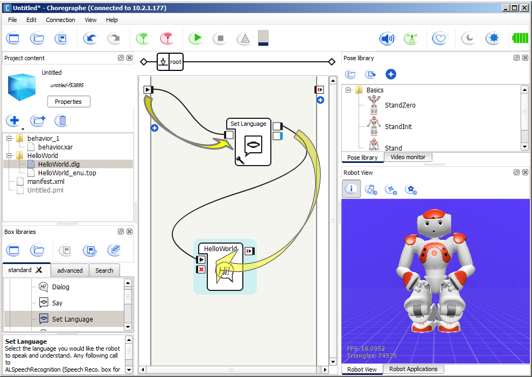
\includegraphics[width=\textwidth]{assets/helloworld_cho_dlg_05.png}
% %http://doc.aldebaran.com/2-1/getting_started/helloworld_choregraphe_dialog.html
% \caption{Choreographe Albebaran}
% \label{fig:choreographe}
% \end{subfigure}%
% \begin{subfigure}[b]{0.5\textwidth}
% 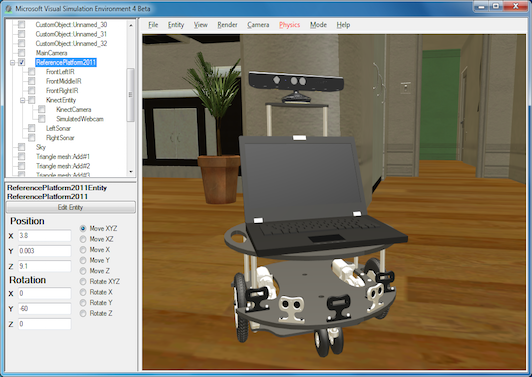
\includegraphics[width=\textwidth]{assets/MSRD4_VSE2.png}
% %http://www.microsoftstore.com/store/msusa/en_US/pdp/Kinect-for-Windows-v2-Sensor/productID.298810500
% \caption{MSRD Studio 4:Visual Simulation Environment}
% \label{fig:msrd4_vse}
% \end{subfigure}%
% \caption[Visual Programming Tools]{Visual Programming Tools. {Adapted from manufacturer's site}}
% \label{fig:visprog}
% \end{figure}
A non-domain-specific solution called \emph{Targets-Drives-Means (TDM)} is proposed in \cite{berenz2014targets} taking into account the aforementioned needs. TDM proposes a programming paradigm where temporal independent dynamic behaviors blocks run in parallel. The logic of the program is not expressed using communication links in a flowchart, but by the use of specialized dynamic components that regulate the activation status and the priorities of the behaviors. The information exchange occurs via a specialized centralized memory called \emph{Internal Model(IM)} which takes care of asynchronous information flow (push/pull communication) between connected components, odometry, object permanence, and activation of behaviors through triggers. However there does not exist an intuitive interface for the behavior design yet. Moreover the information from the authors indicate that this framework will be copyrighted and will not be open.
% \begin{figure}[H]
% \centering
% 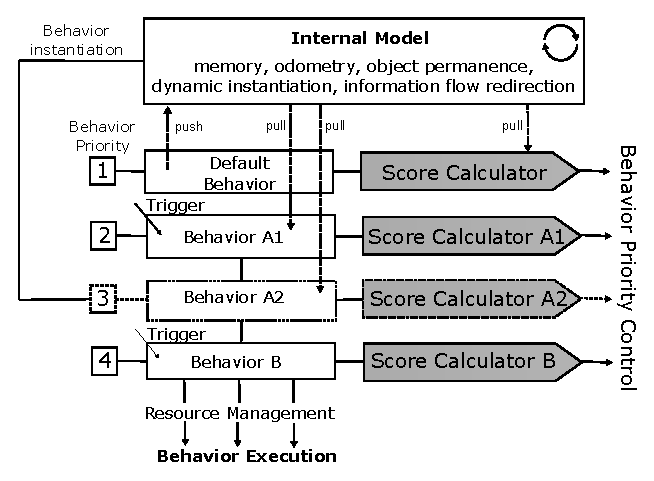
\includegraphics[width=0.5\textwidth]{assets/tdm_im.eps}
% \caption[Target-drives-means Framework]{TDM Framework. {Adapted from \cite{berenz2014targets}}}
% \label{fig:tdm_im}
% \end{figure}

\section{HRI Design and Evaluation} % Main chapter title
Human-Robot Interaction (HRI) being a rapidly advancing area of research, there is a growing need for strong experimental designs and methods of evaluation. This will bring credibility and validity to scientific research that involves humans as subjects, as recognized in the psychology and social science fields. Some methods of evaluation have been adopted and/or modified from such fields as human-computer interaction, psychology, and social sciences; however, the manner in which a human interacts with a robot is similar but not identical to interactions between a human and a computer or a human interacting with another human. It often has a strong social or emotional component - a difference that poses potential challenges related to the design and evaluation of HRI. As robots are becoming more prevalent, accurate methods to assess how humans respond to robots, how they feel about their interactions with robots, and how they interpret the actions of robots are very important. 
%\subparagraph{Planning, Design and Data collection}
A successful human study in HRI requires careful planning and design. In \cite{bethel2010review}, a set of questions when planning and designing a human study in HRI is presented. Apart from providing a checklist for planning and design of HRI studies, a list of recommendations for the experimental design and study execution is also provided in \cite{bethel2010review}.
	
Data collection is one of the important steps in the evaluation process. In \cite{Rogers2011} which provides insights into designing interative systems, five key issues in the data gathering has been described. They are 
\begin{itemize}
\item \emph{Identifying participants} : Decide who to gather data from
\item \emph{Relationship with participants} : Establishing a clear and professional relationship
\item \emph{Setting goals} : Deciding how to analyze data once collected, Informed consent when appropriate
\item \emph{Triangulation} : Looking at data from more than one perspective
\item \emph{Pilot studies} : Small trial of main study. 
\end{itemize}

An extensive review of HRI evaluation methods presented in \cite{bethel2010review} summarises five primary methods such as \emph{Self assessments}, \emph{Interviews}, \emph{Behavioral measures}, \emph{Psychophysiology measures} and \emph{Task performance metrics}. Each of these methods has advantages and disadvantages. However the study claims that it is possible to overcome these disadvantages by using three or more appropriate methods of evaluation. An effort to identify a set of common metrics to be used in task-oriented HRI can be found in \cite{Steinfeld2006}. This study proposes a set of metric to evaluate the human-robot team and human-robot interactions and those proposed metrics are shown in Table~\ref{table:hri_metrics}
\begin{table}[H]
\centering
\small
\caption{Common metrics for task-based HRI}
\label{table:hri_metrics}
\begin{tabularx}{400pt}{c*3{X}}
\toprule
  \textbf{Common metrics} & \textbf{Sub-metrics} 
                          & \textbf{Description}
  \tabularnewline \midrule
  
  \multirow{4}{*}{System Performance} & Quantitative performance & Assess the effectiveness and efficiency at performing a task. \\
                                      & Subjective ratings & Assess the quality of the effort. \\
                                      & Utilization of mixed-initiative & Ability of the human-robot team to appropriately regulate who has control initiative. 
                                          \tabularnewline\midrule
                                          
  \multirow{4}{*}{Operator Performance} & Situation Awareness (SA) & The degree to which the robot is situation aware. \\
                                        & Workload & Relating human perceptions of cognitive load to operator SA \\
                                        & Accuracy of mental models & Impact of Design affordances, operator expectations and stimulus-response compatibility.
                                          \tabularnewline\midrule
  
  \multirow{4}{*}{Robot Performance}  & Self Awareness & The degree to which a robot can accurately assess itself \\
                                      & Human Awareness & The degree to which the robot is aware of humans \\
                                      & Autonomy & The ability of robots to function independently without human intervention.
                                          \tabularnewline                                
                                         
  										\bottomrule
\end{tabularx}
\end{table}
Bartneck et al., \cite{bartneck2009measurement} emphasize the need for standardized measurement tools for human robot interaction. The main contribution of this work is that it presents measurements tools of five key concepts in HRI: anthropomorphism, animacy, likeability, perceived intelligence, and perceived safety. The outcome of the work is basically five consistent questionnaires using semantic differential scales. Moreover the study also reported reliability and validity indicators based on several empirical studies that used these questionnaires. Specifically, this study uses \emph{Cronbach's alpha} to estimate the reliability of the questionnaires. The results presented in the study showed that the developed questionnaires to measure the aspects have sufficient internal consistency reliability. All the evaluation techniques rely on the statistical tools for validating the results and generalizing the phenomena. A summary of statistical tools for the data analysis in HRI can be found in Appendix~\ref{AppendixA}.


\section{Summary}

In this chapter a review of the literature which are most relevant to this thesis research is presented. The literature review helped to identify the appropriate techniques that could be used in the development of experimental platform. The key decisions made are shown in the Table~\ref{table:review_decisions}

\begin{table}[H]
\centering
\small
\caption{Identified techniques from state-of-the-art}
\label{table:review_decisions}
\begin{tabularx}{400pt}{|X|X|}
\hline
  \textbf{Problem to be addressed} & \textbf{Identified solution}
  \tabularnewline \hline
  
  \multirow{1}{*}{Human motion understanding} & The Kinect SDK \cite{KinectSDK2014} will suffice the human skeleton tracking. The Visual gesture builder tool that is shipped with Kinect SDK could be used for gesture creation and recogntion
                                          \tabularnewline\hline
                                          
  \multirow{1}{*}{Localization of humanoid robot} & The artificial marker based approaches seems to be the cheapest solution since we will be sharing the same sensor for motion recogntion as well. The ALVAR marker tracking library \cite{ALVAR} will be used for localization of the robot. 
                                          \tabularnewline\hline
  
  \multirow{1}{*}{Application infrastructure} & It has been decided to develop a proprietary application infrastructure as existing solutions like ROS \cite{quigley2009ros} is not cross-platform and the Kinect sensor drivers for Linux are not mature enough at the time of this writing.
                                          \tabularnewline\hline

  \multirow{1}{*}{Behavior framework} & It has also been decided to develop a behavior design and execution framework as the existing solutions are not complete and they do not offer an end-to-end solution for naive users wanting to design HRI scenarios.
                                          \tabularnewline\hline

  \multirow{1}{*}{HRI evaluation} & The \emph{Self-assessment} techniques will be adopted and data collection will be done on a set of identified participants. Statistical analysis will be performed on the collected data.
                                          \tabularnewline\hline
\end{tabularx}
\end{table}
% Chapter Template

\chapter{System Implementation} % Main chapter title

\label{Chapter4} % Change X to a consecutive number; for referencing this chapter elsewhere, use \ref{ChapterX}

\lhead{Chapter 4. \emph{System Implementation}} % Change X to a consecutive number; this is for the header on each page - perhaps a shortened title
The software framework proposed and introduced in \ref{Chapter4} has been exploited to develop the experimental platform. In this chapter the software architecture of the experimental platform is presented. Apart from the architecture itself, specific implementation details of each of the components in the system is also described in this chapter.  The software is designed using a hierarchical structure. The main layers of the system are
\begin{itemize}
\item \emph{Hardware Layer} is composed of sensors and robots connected to the network. Currently only those sensors that support TCP/IP network communication are considered.
\item \emph{Distributed Components Layer} is composed of individual processes that could be running across different computers/devices in the network
\item \emph{Application Components Layer} is the central server of the experimental platform which contains the backend processing units for the application to run as a whole.
\item \emph{User Interface Layer} takes the responsibility of providing useful and intuitive user-interface to the end users.
\end{itemize}
The architecture of the system shown in Fig~\ref{fig:architecture}. More finer details of each of the layers are presented in the following Sections~\ref{ssec:app_comp}$\sim$\ref{ssec:ui_comp}.

\begin{figure}
\centering
\begin{subfigure}[t]{0.48\textwidth}
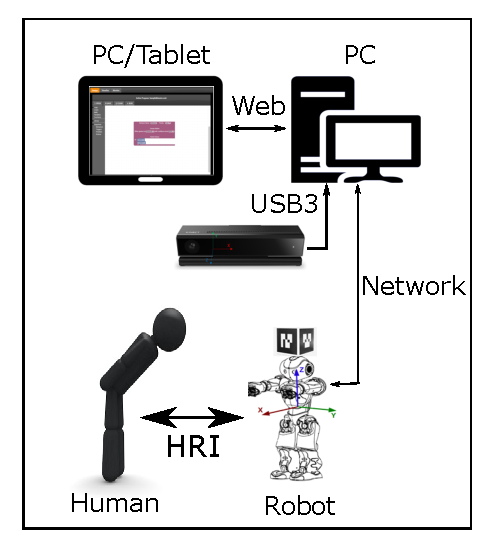
\includegraphics[width=\textwidth]{../thesis/assets/system_setup.eps}
\caption[System setup]{System setup}
\label{fig:localize_frames}
\end{subfigure}
\begin{subfigure}[t]{0.48\textwidth}
\includegraphics[width=\textwidth]{../thesis/assets/architecture.eps}
\caption[Software architecture]{Software architecture}
\label{fig:architecture}
\end{subfigure}
\caption[Experimental platform]{Experimental platform}
\label{fig:nao_localization}
\end{figure}
% \begin{figure}
% \centering
% \includegraphics[width=0.7\textwidth]{assets/architecture.eps}
% \caption[System Architecture]{System Architecture}
% \label{fig:architecture}
% \end{figure}
\section{Application Components}
\label{ssec:app_comp}
The application level components are responsible for bootstrapping and maintain the uptodate status of the system. 
\subsection*{Context}
The application context contains the complete description of the world. It contains latest information about
\begin{itemize}
\item Robot(s): A list of robots in the environment along with their 6D pose, Sensor information like Joint values etc.,
\item Human(s): A list of humans with their Skeleton Positions and Orientation, Active Gestures/Motions
\item Object(s): A list of manipulable objects in the environment along with their properties like description, color etc.,
\item Gesture Modules : A set of gesture recognition modules registered in the system that can actively provide information about the gestures of the humans in the environment.
\item Robot Behavior Modules: A set of robot behavior execution modules registered in the system.
\end{itemize}
The data structure of the context is shown in Fig~\ref{fig:system_context}
\begin{figure}
\centering
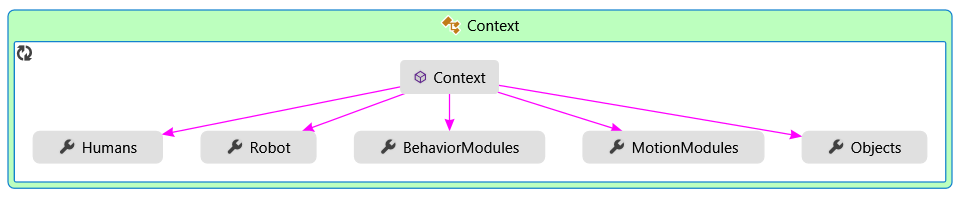
\includegraphics[width=\textwidth]{assets/context_diagram.png}
\caption[Application Context]{Application Context}
\label{fig:system_context}
\end{figure}
\subsection*{Parameter Server} 
The parameter server acts as a central repository for managing the parameters of the system and of the distributed components. The parameter server is basically designed as a responder socket which responds to the requests from a remote client. The list of supported request to pull the data from the parameter server is shown in the Table~\ref{table:parameter_server}
\begin{table}[H]
\centering
\small
\caption{Parameter server interface specification}
\label{table:parameter_server}
\begin{tabular}{| p{3.1cm} | p{7.4cm} | p{2.8cm} |}
\hline
  \textbf{Request Description} & \textbf{Request Arguments} & \textbf{Response}
  \tabularnewline \hline
  Node Parameters request & \begin{itemize}[leftmargin=*,topsep={0pt},itemsep={0pt},partopsep={0pt},parsep={0pt}] 
                                                  \item Name of the node: string
                                                  \end{itemize} & Node Parameters 
                                          \tabularnewline\hline
                                          
  Motion recognition module registration request &  \begin{itemize}[leftmargin=*,topsep={0pt},itemsep={0pt},partopsep={0pt},parsep={0pt}] 
                                                  \item Name of the node: string
                                                  \item Module Information: GestureRecognitionModule
                                                \end{itemize} & Registration Status  (Success/Failure)
                                          \tabularnewline\hline
  
  Robot Interface module registration request & \begin{itemize}[leftmargin=*,topsep={0pt},itemsep={0pt},partopsep={0pt},parsep={0pt}] 
                                                \item Name of the node: string
                                                \item Module Information: RobotBehaviorModule 
                                            \end{itemize} & Registration Status  (Success/Failure)
                                          \tabularnewline\hline
  File Request & \begin{itemize}[leftmargin=*,topsep={0pt},itemsep={0pt},partopsep={0pt},parsep={0pt}] 
                                                  \item Name of the file
                                                  \end{itemize} & Contents of the File  
  										 \tabularnewline\hline
\end{tabular}
\end{table}
\subsection*{Context Orchestrator} The orchestrator collect uptodate information about the robots and humans in the environment from the perception system and updates the Context. The algorithm used by the orchestrator to update the context information is shown below.

\begin{algorithm}[H]
 \KwData{(app\_config, context)}
 \textbf{\emph{Init}}:\\
 \quad PUBLISHERS = READ\_ALL\_PUBLISHER\_INFO(app\_config)\;
 \quad SUBSCRIBERS = CREATE\_SUBSCRIBERS(PUBLISHERS)\;
 \While{run}{
 	\ForAll{SUBSCRIBER in SUBSCRIBERS}{ 
 		data = RECEIVE\_DATA(SUBSCRIBER,TIME\_OUT)\;
 		UPDATE\_CONTEXT(context, data)\;
 	}
 }
 \caption{Context Synchronization Algorithm}
 \label{alg:context_sync}
\end{algorithm}
\subsection*{Embedded Web server}
The web server embedded in the application serves the file and data requests from the web client. The server side server implements a set of RESTful services which could be accessed from the web clients. The JSON data format which is the default standard for modern web interface development has been used as data exchange format between the server and the web clients. The list of RESTful API implemented on the server side is shown in Table~\ref{table:restful_api}
\begin{table}[H]
\centering
\small
\caption{Embedded Web Server RESTful API}
\label{table:restful_api}
\begin{tabular}{|l|p{2.8cm}|p{1.2cm}|p{5.5cm}|}
\hline
  \textbf{Request Url}  & \textbf{Parameters} & \textbf{Request Type} & \textbf{Description/Response}
  \tabularnewline \hline
  /models/{type}/(?$<$all$>$.*) & File Name & GET & Robot 3D Model Data
                                          \tabularnewline\hline
                                          
  /context  & - & GET & Current context data  
  										                    \tabularnewline\hline
  										 
  /robot  &  - & GET & Default Robot information  
  										                    \tabularnewline\hline										 
  
  /humans & - & GET  & Information about all the human in the environment  
                                          \tabularnewline\hline
                                          
  /human/\{id\} & id - Human Id & GET  & Information about the human with the given id.  
                                          \tabularnewline\hline
                                          
  /jointvals & - & GET  & Joint values of the default robot  
                                          \tabularnewline\hline
                                          
  /visualize/skeleton/list & - & GET  & 3D Skeleton positions of all the humans in the environment  
                                          \tabularnewline\hline                                        
       
  /designer/program/list & - & GET  & List of all the behavior programs stored in the server  
                                          \tabularnewline\hline                                                               
                                          
  /designer/program/start & Behavior Program & POST  & Request the bootstrapper to start the program
  										                    \tabularnewline\hline   

  /designer/program/save & File Name, Behavior Program & POST  & Request the bootstrapper to start the program
                                          \tabularnewline\hline 
  /designer/program/stop & - & POST  & Request to stop running program if any
                                          \tabularnewline\hline
\end{tabular}
\end{table}

\subsection*{Bootstrapper} 
The bootstrapper takes care of initializing the system and starting up all the pre-configured nodes. The configuration information of the nodes is specified using the XML configuration file described in Section~\ref{sec:config_file}. It also takes of starting and stopping the behavior programs when requested by the user. The sequence operations of bootstrapper performs is represented in Algorithm~\ref{alg:bootstrapper}.

\begin{algorithm}[H]
 \KwData{(XML Config File)}
 \textbf{\emph{Startup}}:\\
 \quad INIT\_AND\_RUN\_PARAMETERSERVER()\;
 \quad INIT\_AND\_RUN\_CONTEXTSYNC()\;
 \quad INIT\_AND\_RUN\_CONTEXTSERVER()\;
 \quad INIT\_AND\_RUN\_WEBSERVER()\;
 \quad NODES = GET\_NODES(XML Config File)\;
 \quad PROCESSES = []\;
 \ForAll{NODE in NODES}{ 
 	\If{NODE is ENABLED}{
 		PROCESS = CREATE\_PROCESS(NODE)\;
 		APPEND(PROCESSES, PROCESS)
 	} 
 }
 \While{run}{
 	MONITOR(PROCESSES)
 }
 \textbf{\emph{Shutdown}}:\\
 \quad SHUTDOWN\_WEBSERVER()\; 
 \quad SHUTDOWN\_CONTEXTSERVER()\;
 \quad SHUTDOWN\_CONTEXTSYNC()\;
 \quad SHUTDOWN\_PARAMETERSERVER()\;
 \quad SHUTDOWN(PROCESSES)
 \caption{Bootstrapper Algorithm}
 \label{alg:bootstrapper}
\end{algorithm}
\section{Distributed Components}
\label{ssec:dist_comp}
These are nodes in the system each with a specific goal that can be started/stopped at any time during the entire application life-cycle without affecting the other nodes or the system. All the nodes will communicate with the application using message passing techniques. They can run in any machine inside the network.

\subsection{Motion Recognition Node} A dedicated node that interacts with a motion recognition sensor and sends the detected gestures and motions to the application. Additionally each motion recognition module registers a set of actions/gestures that could be detected with the sensor associated with it. The gesture recognition logic depends on the sensor associated with the gesture recognition module. The gesture recognition workflow of kinect based system in explained in Section~\ref{sssec:kinect_gestures}
\subsubsection{Kinect Gesture Recognition}
\label{sssec:kinect_gestures}
	The Microsoft Kinect system utilizes Adaptive Boosting(adaboost) algorithm \cite{freund1997decision} to efficiently detect the gestures. The system involves a training phase during which the desired gestures are captured and tagged. These tagged gestures will be used by a gesture detector trainer which will generate a set of training examples. The training results are stored in files and will be used by the gesture detector to perform per-frame classification of the data. The Visual Gesture Builder (VGB) tool that comes together with Kinect for Windows SDK eases the process of tagging the gestures, evaluating the gesture recognition and creating the gesture database. The work-flow of using the VGB is shown in the Figure~\ref{fig:vgb_workflow}.
\begin{figure}[H]
\centering
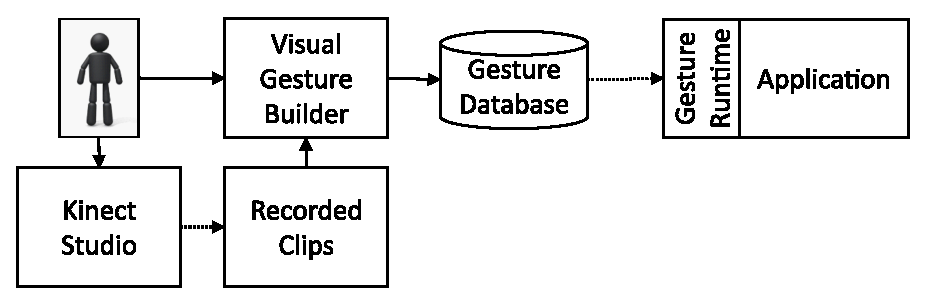
\includegraphics[width=0.8\textwidth]{assets/vgb_flow.eps}
\caption[Visual Gesture Builder Work flow]{Visual Gesture Builder Work flow \cite{KinectSDK2014}}
\label{fig:vgb_workflow}
\end{figure}
% Motion recognition
The workflow shown in Figure~\ref{fig:vgb_workflow} has been adopted to develop all the gestures needed for the kinect gesture recognition module. The process followed for generating the Left hand wave gesture is shown in the Figure~\ref{fig:gesture_waveleft}. As shown in the figure at first the clips are captured using the Kinect studio tool and  stored as \textbf{XEF} files. The clips are then imported in the visual gesture builder. The imported clips could be traversed and the tagging is done (i.e at each frame it is possible to specify if that particular frame is part of the gesture of interest or not). This process could be repeated on one or more imported clips. The tagged clips are built in order to generate a set of weak classifiers and learn confidence values for each of those classifiers. Once the training process is complete, the trained classifier could be evaluated over a set of test clips using a live preview as shown in step 3 in the figure. When the results are satisfactory, the training data could be exported as a database saved as \textbf{VGD} (Visual Gesture Database) format.
\begin{figure}[H]
\centering
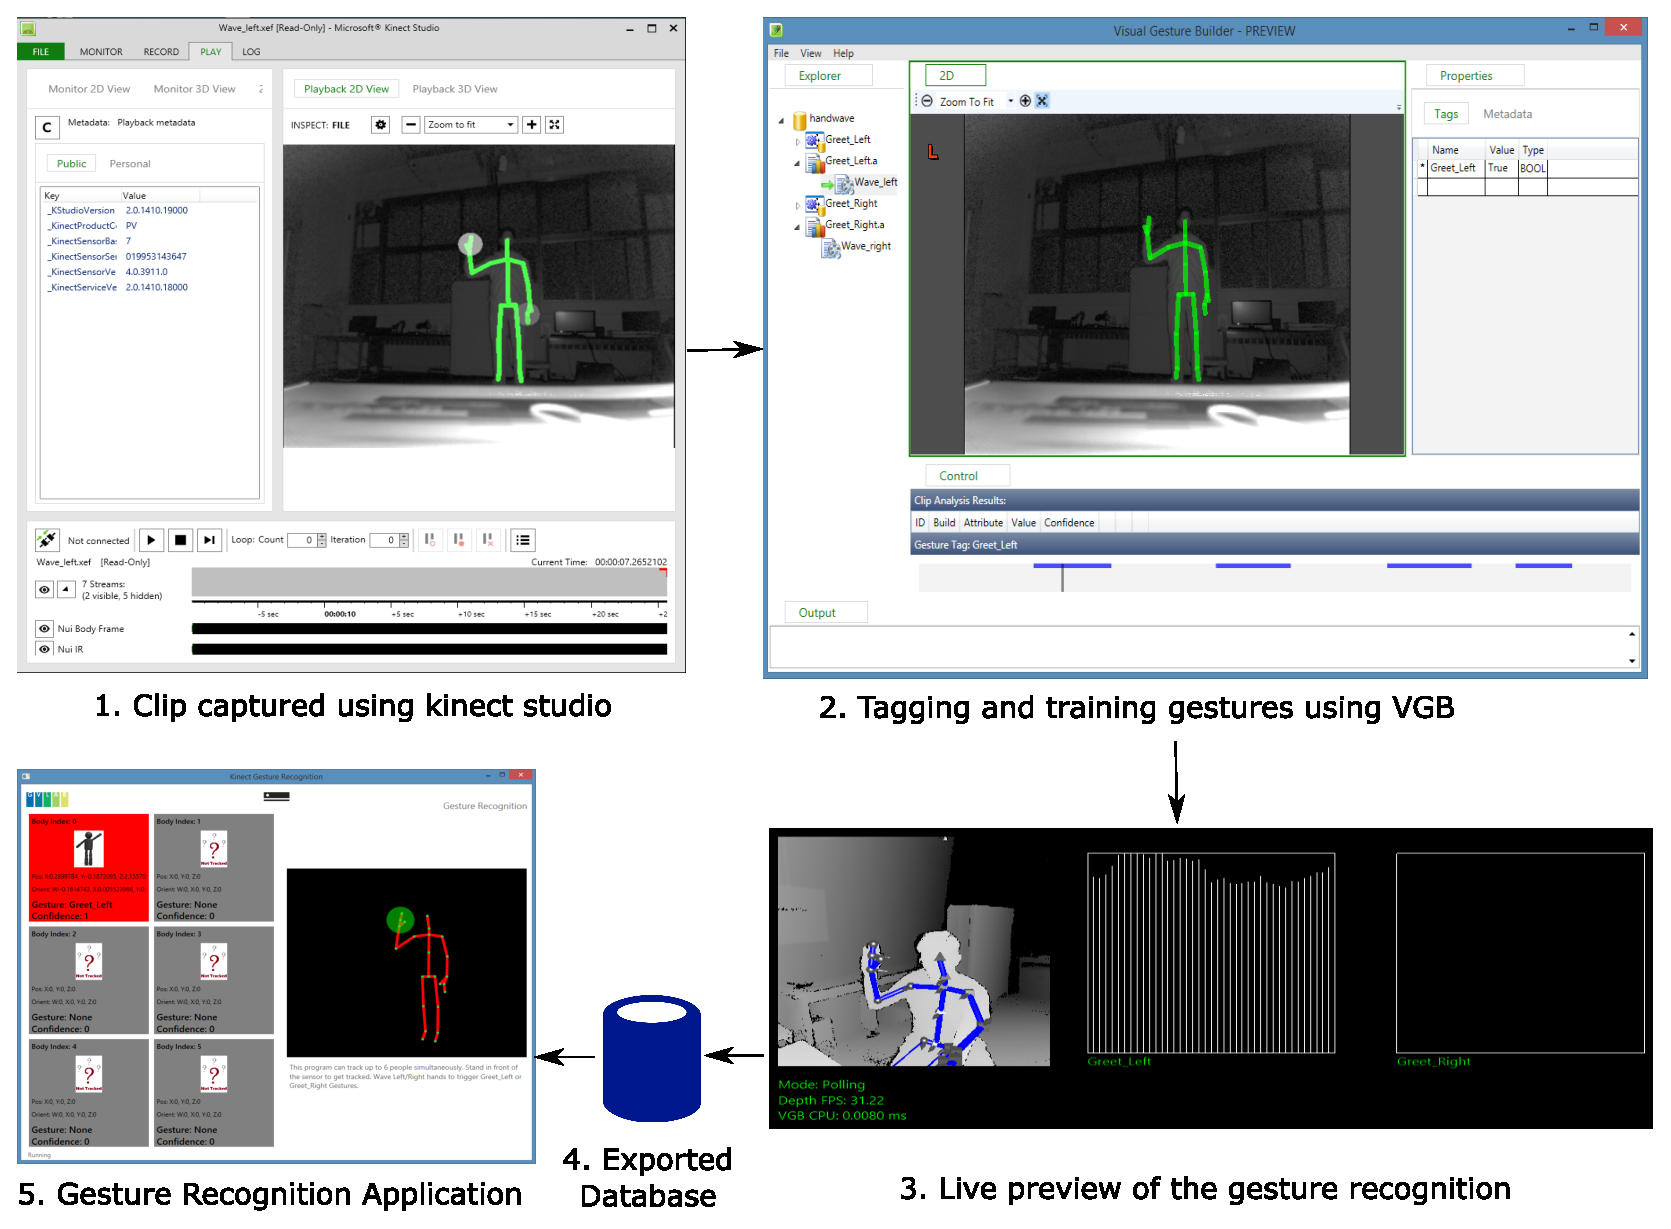
\includegraphics[width=\textwidth]{assets/gesture_recog_flow.eps}
\caption[Left hand wave gesture work flow]{Left hand wave gesture work flow}
\label{fig:gesture_waveleft}
\end{figure}
The database is imported into the gesture recognition module and the responsibility of this module is to notify any interested subscribers when a gesture is recognized. Additionally this module also publishes information about the skeletons of the humans in view. The algorithm of this module is shown in Algorithm~\ref{alg:gesture_recognize}

\begin{algorithm}[H]
 \KwData{Gesture database}
 \KwResult{Gesture Triggers}
 \textbf{\emph{Init}}:\\
 \quad gestures = READ\_DATABASE()\;
 \quad REGISTER\_GESTURES(gestures)\;
 \While{True}{
  skeletons = GET\_SKELETONS()\;
  \ForAll{gesture in gestures}{ 
    detected = DETECT\_GESTURE(gesture)\;
    \If{detected}{
      PUBLISH(gesture)\;
    } 
  }
  PUBLISH(skeletons)\;
 }
 \caption{Kinect Gesture Recognition Module}
 \label{alg:gesture_recognize}
\end{algorithm}
\subsection{Robot interface node} 
The Robot interface node is a dedicated node that interacts with a specific robot and can invoke a set of actions on it.  It registers a set of actions that could be invoked on the robot associated with it. The robot interface node sets up a publisher that periodically sends the information about the robot status like joint values, sensor information to the application to keep the context uptodate. Additionally it sets up a responder socket which will wait for action execution request from the remote node. 
\begin{figure}[H]
\centering
\begin{tikzpicture}[->,shorten >=1pt,auto,node distance=4cm,thick]
%\tikzstyle{every state}=[fill=gray,draw=none,text=black]
\tikzstyle{every state}=[circle,minimum size=1.5cm,text=black]
\node[initial,state] (A) {$idle$};
\node[state] (B) [above right of=A] {$wait$};
\node[state] (C) [below right of=B] {$error$};
\node[state] (D) [above right of=C] {$ready$};
\node[state] (E) [below right of=C] {$run$};
\node[state] (F) [below right of=A] {$stop$};
\path 
(A) edge [bend right] node {\textbf{on\_start\_req}} (B)
    %edge [loop below] node {} (A)
    
(B) edge node {\textbf{on\_args}} (D)
    edge [left,bend left] node {\textbf{on\_err}} (C)
    %edge [loop above] node {} (B)
    
(C) edge node {\textbf{on\_reset}} (A)
    %edge [loop above] node {1,0,R} (C)
    
(D) edge [bend left] node {\textbf{on\_run\_req}} (E)
  edge [right,bend right] node {\textbf{on\_err}} (C)
  %edge [loop above] node {1,1,R} (E)

(E) edge [bend left=70] node {\textbf{on\_task\_fin}} (A)
    edge node {\textbf{on\_stop\_req}} (F)
    edge [right,bend left] node {\textbf{on\_err}} (C)
    
(F) edge [left,bend right] node {\textbf{on\_err}} (C)
    edge  [bend right] node {\textbf{on\_stopped}} (A)  
    %edge [loop below] node {1,0,R} (E)
;
\end{tikzpicture}
\caption[Finite state machine of robot interface node]{Finite state machine of robot interface node}
\label{fig:robot_fsm}
\end{figure}
The robot interface node implements a Finite state machine (Figure~\ref{fig:robot_fsm}) in order appropriately streamline the data/status management with the remote caller node. The states of the FSM are
\begin{itemize}
\item \emph{idle:} The robot is ready to receive new execution request.
\item \emph{wait:} The node is waiting for the action execution arguments.
\item \emph{error:} The node/robot has encountered an error during execution.
\item \emph{ready:} The robot is waiting for the run trigger.
\item \emph{run:} The robot is executing the requested task.
\item \emph{stop:} The robot is stopping execution
\end{itemize}
Each of the above states has a self loop when waiting for the state transition trigger. It is not shown in the figure for brevity. The events that causes the state transition in the FSM are
\begin{itemize}
\item \emph{on\_start\_req:} Received start execution request
\item \emph{on\_args:} Received task execution arguments.
\item \emph{on\_run\_req:} Received run task request.
\item \emph{on\_task\_fin:} Task execution completed
\item \emph{on\_stop\_req:} Received stop execution request. This is served with high priority.
\item \emph{on\_stopped:} The task stop operation completed
\item \emph{on\_reset:} Received error reset request
\item \emph{on\_err:} An error occured during the execution
\end{itemize}
The robot interface node dedicated to Nao humanoid robot is described in Section~\ref{sssec:nao_interface}
\subsubsection{NAO Robot Interface}
\label{sssec:nao_interface}
The Nao robot interface makes use of the NaoQi python SDK which provides API for accessing various functionalities of the robot such as joint/cartesian control, memory access, motion, speech, object/face/people detection and tracking, behavior invocation etc., A set of necessary functions are implemented in the NaoBehaviorModule and they are registered to the application when the node is started up. The control flow is shown in Figure~\ref{fig:nao_interface}.
\begin{figure}[H]
\centering
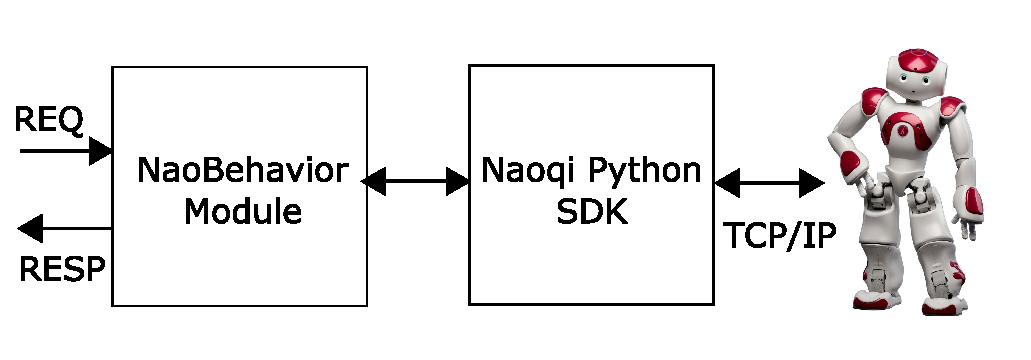
\includegraphics[width=0.7\textwidth]{assets/NaoBehaviorModule.eps}
\caption[NAO Robot Interface]{NAO Robot Interface}
\label{fig:nao_interface}
\end{figure}
The visual representation of a set of action blocks developed for Nao humanoid robot is illustrated in Section~\ref{sec:block_impl}
% \begin{center}
% \begin{tikzpicture}[scale=0.2]
% \tikzstyle{every node}+=[inner sep=0pt]
% \draw [black] (55.7,-14.6) circle (3);
% \draw (55.7,-14.6) node {$WAIT\_ARG$};
% \draw [black] (35.2,-3.8) circle (3);
% \draw (35.2,-3.8) node {$IDLE$};
% \draw [black] (35.2,-3.8) circle (2.4);
% \draw [black] (55.7,-38.7) circle (3);
% \draw (55.7,-38.7) node {$RUN\_READY$};
% \draw [black] (32.9,-48.5) circle (3);
% \draw (32.9,-48.5) node {$RUN$};
% \draw [black] (28.9,-25.4) circle (3);
% \draw (28.9,-25.4) node {$STOP$};
% \draw [black] (44.7,-25.4) circle (3);
% \draw (44.7,-25.4) node {$ERROR$};
% \draw [black] (57.005,-17.299) arc (22.31081:-22.31081:24.631);
% \fill [black] (57,-36) -- (57.77,-35.45) -- (56.85,-35.07);
% \draw (59.35,-26.65) node [right] {$ON\_ARGS$};
% \draw [black] (38.197,-3.731) arc (87.25861:37.17824:21.184);
% \fill [black] (54.06,-12.09) -- (53.98,-11.15) -- (53.18,-11.75);
% \draw (53.19,-5.63) node [above] {$START\_REQ$};
% \draw [black] (33.218,-51.471) arc (33.84033:-254.15967:2.25);
% \draw (25.82,-55.47) node [below] {$RUNNING$};
% \fill [black] (30.73,-50.56) -- (29.79,-50.59) -- (30.35,-51.42);
% \draw [black] (29.936,-48.053) arc (-102.41345:-263.47757:22.391);
% \fill [black] (32.21,-3.94) -- (31.35,-3.53) -- (31.47,-4.53);
% \draw (11.81,-25.01) node [left] {$TASK\_FIN$};
% \draw [black] (32.39,-45.54) -- (29.41,-28.36);
% \fill [black] (29.41,-28.36) -- (29.06,-29.23) -- (30.04,-29.06);
% \draw (30.18,-37.19) node [left] {$STOP\_REQ$};
% \draw [black] (27.383,-27.975) arc (-2.77501:-290.77501:2.25);
% \draw (22.64,-30.42) node [left] {$STOPPING$};
% \fill [black] (25.93,-25.76) -- (25.16,-25.22) -- (25.11,-26.22);
% \draw [black] (29.74,-22.52) -- (34.36,-6.68);
% \fill [black] (34.36,-6.68) -- (33.66,-7.31) -- (34.62,-7.59);
% \draw (31.28,-14.02) node [left] {$STOPPED$};
% \draw [black] (54.018,-41.181) arc (-38.28052:-95.20104:20.74);
% \fill [black] (35.86,-48.99) -- (36.61,-49.56) -- (36.7,-48.56);
% \draw (50.89,-47.95) node [below] {$RUN\_REQ$};
% \draw [black] (53.79,-36.39) -- (46.61,-27.71);
% \fill [black] (46.61,-27.71) -- (46.74,-28.65) -- (47.51,-28.01);
% \draw (50.75,-30.62) node [right] {$ON\_ERR$};
% \draw [black] (53.56,-16.7) -- (46.84,-23.3);
% \fill [black] (46.84,-23.3) -- (47.76,-23.09) -- (47.06,-22.38);
% \draw (45.79,-19.52) node [above] {$ON\_ERR$};
% \draw [black] (31.9,-25.4) -- (41.7,-25.4);
% \fill [black] (41.7,-25.4) -- (40.9,-24.9) -- (40.9,-25.9);
% \draw (36.8,-25.9) node [below] {$ON\_ERR$};
% \draw [black] (43.49,-22.65) -- (36.41,-6.55);
% \fill [black] (36.41,-6.55) -- (36.27,-7.48) -- (37.19,-7.08);
% \draw (40.68,-13.62) node [right] {$RESET$};
% \draw [black] (34.26,-45.83) -- (43.34,-28.07);
% \fill [black] (43.34,-28.07) -- (42.53,-28.56) -- (43.42,-29.01);
% \draw (39.49,-38.08) node [right] {$ON\_ERR$};
% \end{tikzpicture}
% \end{center}
\subsection{Localization Node} A dedicated node which uses the perception system to resolve and publish the current position of the robot.
\subsubsection{NAO Robot localization}
The fiducial marker based approach is used in order to localize the robot in the field of view of the Kinect sensor. The ALVAR \cite{ALVAR} toolkit is used for marker detection purpose which relies on OpenCV library for image processing. The OpenCV library cannot directly read the image streams from Kinect sensor and hence a OpenCV compatible driver is implemented to read the RGB image streams. The first step in the marker detection is to calibrate the camera in order to get its intrinsic parameters and the calibration parameters are stored in an XML file. A set of supported markers of known identifiers are chosen and a cube of known geometry is created. The cube is designed in such a way that at any instant atleast one of the markers will be detected if the robot is in the detectable range of the camera. The cube is mounted on the head of NAO robot since it will avoid the problem of occlusion in most cases. However since the head of the NAO has 2 DOF which will result in the movement of mounted cube even if the robot itself does not move. In order to overcome this problem, a kinematic model of the NAO humanoid robot from torso frame to tip of the head frame parameterized using Modified Denavit Hartenberg (MDH) \cite{khalil2004modeling} parameters is used. The MDH parameters are shown in Table~\ref{table:nao_mdh}.
\begin{table}[H]
\centering
\small
\caption{MDH parameters from Torso to top of head}
\label{table:nao_mdh}
% \begin{tabular}{|l|l|p{1cm}|p{1cm}|p{1cm}|p{1cm}|p{3cm}|}
\begin{tabular}{|l|l|c|c|c|c|p{2cm}|}
\hline
  \textbf{$i$}  & \textbf{$j$}  & \textbf{$\alpha_j$ (rad)} & \textbf{$d_j$ (mm)} & \textbf{$\theta_j$ (rad)} & \textbf{$r_j$ (mm)} & \textbf{Description}
  \tabularnewline \hline
  - & 0 & 0 & 0 & 0 & 0 & Torso/Base
                                          \tabularnewline\hline
                                          
  0 & 1 & 0 & 0 & $\theta_1$ & 126.50 & Head Yaw
                                          \tabularnewline\hline
                       
  1 & 2 & $-\frac{\pi}{2}$ & 0 & $\theta_2$ & 0 & Head Pitch
                                          \tabularnewline\hline                    
  
  2 & 3 & $\frac{\pi}{2}$ & 0 & 0 & 110.00 & Head Tip
                                          \tabularnewline\hline
\end{tabular}
\end{table}

\begin{figure}
\centering
\begin{subfigure}[t]{0.48\textwidth}
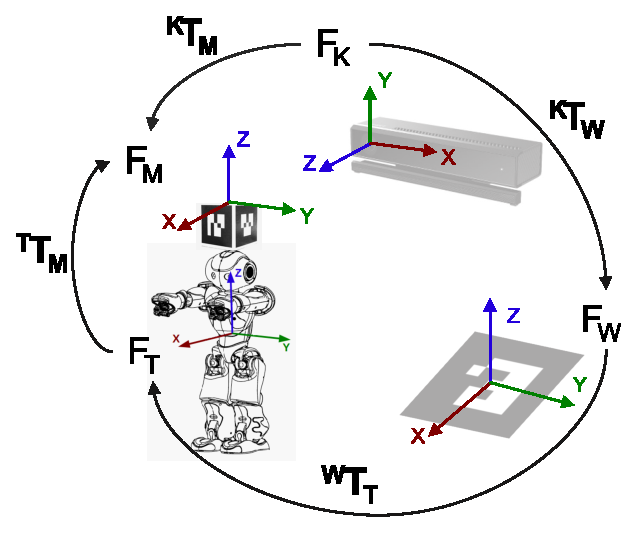
\includegraphics[width=\textwidth]{../thesis/assets/localization_concept2.eps}
\caption[Modeling]{Coordinate Frames}
\label{fig:localize_frames}
\end{subfigure}
\begin{subfigure}[t]{0.48\textwidth}
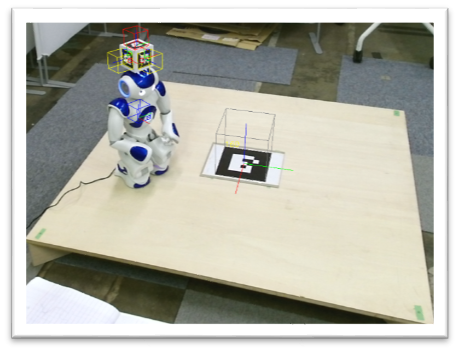
\includegraphics[width=\textwidth]{../thesis/assets/localization_frames.png}
\caption[Actual setup]{Actual setup}
\label{fig:localize_setup}
\end{subfigure}
\caption[NAO robot localization]{NAO robot localization}
\label{fig:nao_localization}
\end{figure}
\subparagraph{Modeling}
For computing the absolute pose of the torso frame of the robot with respect to the world frame, the coordinate frames shown in Figure~\ref{fig:nao_localization} is used. 
\begin{tabular}{r l}
\centering
  Kinect Frame & $F_K$ \\ 
  Marker Frame & $F_M$ \\ 
  Torso Frame & $F_T$ \\ 
  World Frame & $F_W$ \\ 
  Transformation Matrices  & ($^{K}T_M$,$^{T}T_M$,$^{K}T_W$,$^{W}T_T$) \\
\end{tabular}
The algorithm for the computation given the marker parameters, calibration information of the camera, MDH parameters (Table~\ref{table:nao_mdh}) and the joint values ($\theta_1,\theta_2$) at each time instant is shown in Algorithm~\ref{alg:localize}.
\begin{algorithm}
 \KwData{marker\_size, cube\_size, MDH\_Params}
 \KwResult{TORSO\_POSE}
 \textbf{\emph{Init}}:\\
 g\_model := INIT\_GEOM\_MODEL(MDH\_Params)\;
 m\_model := MARKER\_MODEL(marker\_size, cube\_size)\;
 \While{True}{
 	data = READ\_RGB\_STREAM()\;
  [$\theta_1$,$\theta_2$] = READ\_JOINT\_VALUES()\;
 	marker\_poses = DETECT\_CUBE\_MARKERS(data)\;
  $^{K}T_W$ = DETECT\_WORLD\_MARKER(data)\;
 	$^{K}{T}_{M}$ = TRANSFORM\_TO\_TOP\_FRAME(marker\_poses, m\_model)\;
 	$^{T}{T}_{M}$ = COMPUTE\_TOP\_FRAME(g\_model,$\theta_1$,$\theta_2$)\;
 	$^{K}{T}_{T}$ = $^{K}{T}_{M}$ $\times$ ${^{T}{T}_{M}}^{-1}$\;
  $^{W}{T}_{T}$ = ${^{K}{T}_{W}}^{-1}$ $\times$ ${^{K}{T}_{T}}$\;
 	TORSO\_POSE = MEDIAN\_FILTER($^{W}{T}_{T}$)\;
 	PUBLISH(TORSO\_POSE)\;
 }
 \caption{Localization Algorithm}
 \label{alg:localize}
\end{algorithm}
\section{Behavior Program} 
\label{ssec:behavior_program}
A dynamic component that will be created when the user starts the program he/she designed using the user interface. The declarative description of the behavior is parsed in order to create a memory model. The Behavior program node monitors the application context for the motion triggers and invokes the corresponding robot actions according to the way it is being described in the program.
\begin{figure}
\centering
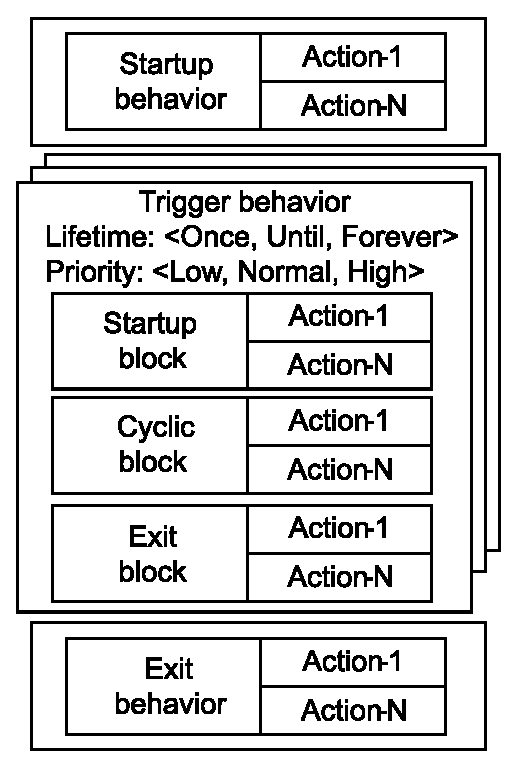
\includegraphics[width=0.4\textwidth]{../thesis/assets/program_structure.eps}
\caption[Behavior Program - Conceptual Model]{Behavior Program - Conceptual Model}
\label{fig:program_concept}
\end{figure}
\subsection{Conceptual Model}
The behavior program is structured in a simple way so that it could be easily understood by the end user. The conceptual model of behavior program is shown in Fig.~\ref{fig:program_concept}. The behavior program is composed of:
\begin{itemize}
\item \emph{Startup behavior}: The startup block will be executed once when the user starts the program. The user can add a set of actions to be performed when the program starts. The start-up block is optional and there cannot be more than one start-up block in the program
\item \emph{Trigger behavior}: The behavior block is the core component of the behavior program. The block could be activated by the interaction between the human and the robot. There could be many behavior blocks in a program. The properties/attributes of a behavior block is shown in Table~\ref{table:behavior_block}.
\begin{table}[H]
\centering
\small
\caption{Trigger Behavior block properties}
\label{table:behavior_block}
\begin{tabular}{|l|p{11cm}|}
\hline
  \textbf{Property} & \textbf{Description}
  \tabularnewline \hline
  
  Trigger & The signal that activates the behavior block. The trigger source could be either of human presence/absence, motion gesture, vicinity of human, verbal command or any boolean edge trigger.
                                          \tabularnewline\hline
                                          
  Lifetime & The lifespan of the behavior block. \begin{itemize}[leftmargin=*,topsep={0pt},itemsep={0pt},partopsep={0pt},parsep={0pt}]
                                                                      \item Once: The block will be executed only once.
                                                                      \item Forever: The block will be executed forever each time trigger condition is met.
                                                                      \item Until: The block will be executed until a condition is met
                                                                   \end{itemize}
                                          \tabularnewline\hline
  
  Priority & The priority of the block could be Low, Normal or High and the behavior execution is scheduled based on fixed-priority preemptive scheduling. There is not dynamic priority allocation as the concept could be confusing for naive users.
                                          \tabularnewline\hline

  Startup & Tasks/actions to be performed once when the block is initialized
                                          \tabularnewline\hline

  Cyclic & Tasks/actions to be performed each time the trigger condition is met
                                          \tabularnewline\hline
  
  Exit &  Tasks/actions to be performed once when the lifetime of the block expires
                                          \tabularnewline                                                                       
                      \hline
\end{tabular}
\end{table}
\item \emph{Exit behavior}: The exit block will be executed once when the lifetime of all the configured behavior blocks expire. Like the startup block there could be only one exit block in the program.
\end{itemize}
\subsection{Block level implementation}
\label{sec:block_impl}
The visual blocks corresponding to each of the startup, trigger and exit behaviors are implemented. The complex programs could be composed by putting together these blocks. The startup and exit blocks are shown in Fig~\ref{fig:blocks_init}. As could be seen from the figure, the blocks are quite simple making it possible to put the list of statements consisting of initialization and termination logic of the program. 
\begin{figure}[H]
\centering
\begin{subfigure}[t]{0.28\textwidth}
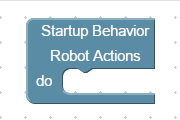
\includegraphics[width=\textwidth]{../thesis/assets/blocks_startup.png}
\caption[Startup block]{Startup block}
\label{fig:program_concept}
\end{subfigure}
\begin{subfigure}[t]{0.28\textwidth}
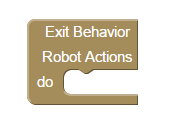
\includegraphics[width=\textwidth]{../thesis/assets/blocks_exit.png}
\caption[Exit block]{Exit block}
\label{fig:program_blocks}
\end{subfigure}
\caption[Startup and Exit behaviors]{Startup and Exit behaviors}
\label{fig:blocks_init}
\end{figure}
The trigger behavior block is designed in such a way that it incorporates the conceptual model and at the same time easier for the end user to understand and use it. The trigger behavior block is shown in Fig~\ref{fig:blocks_trigger}. The visual design provides ability to compose the blocks by putting an external boolean trigger, choose priority and lifetime from the combo box interface, add startup,cyclic and exit statements etc.,
\begin{figure}[H]
\centering
\begin{subfigure}[t]{0.38\textwidth}
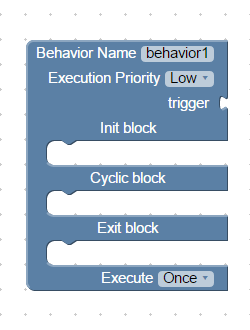
\includegraphics[width=\textwidth]{../thesis/assets/blocks_behavior1.png}
\caption[Example 1]{Priority: Low, Execute: Once}
\label{fig:program_concept}
\end{subfigure}
\begin{subfigure}[t]{0.38\textwidth}
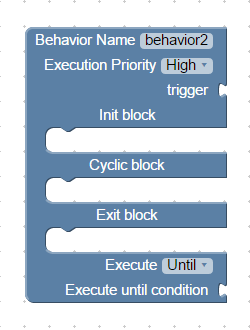
\includegraphics[width=\textwidth]{../thesis/assets/blocks_behavior2.png}
\caption[Example 2]{Priority: High, Execute: Until}
\label{fig:program_blocks}
\end{subfigure}
\caption[Trigger behavior]{Trigger behavior}
\label{fig:blocks_trigger}
\end{figure}
The block interface is reactive in the sense that for instance when the lifetime of the block is switched from \emph{Once/Forever} to \emph{Until}, a new input appears in the block where the user can add the condition to stop the block.

\textbf{TODO: } Describe all the blocks (Triggers/Actions) developed.

\subsection{Code Generation and Execution}
The next step in the behavior program design flow is to generate the executable code from the blocks and execute them. The surface on which the program is designed, is called the \emph{workspace}. Each blocks developed as part of the platform has an associated code generation module. So when the user decides to run a program, as a first step all the blocks in the workspace are iterated and code is generated. The blockly editor supports code generation for programming languages like JS, Python and Dart. However a special code generator that could generate C\# code from the blocks has been. This is because most of the platform is written in C\# and there are loads of goodies that comes with the .NET framework. Traditionally there is a need to compile the C\# code and generate binaries when one wants to execute it. Thanks to the latest compiler technologies and tools like ScriptCS \cite{ScriptCS}, it is now possible to run the C\# code like scripts. This is exploited in the experimental platform to dynamically generate the code and run.
\begin{figure}[H]
\centering
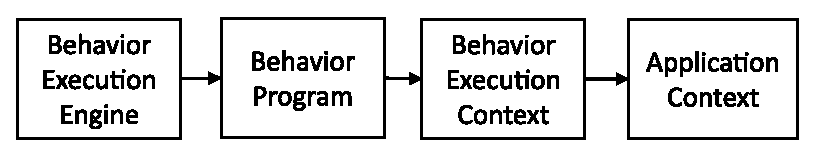
\includegraphics[width=0.8\textwidth]{../thesis/assets/execution_flow.eps}
\caption[Behavior program - Execution flow]{Behavior program - Execution flow}
\label{fig:program_execution}
\end{figure}
 The execution flow of the behavior program is shown in Figure~\ref{fig:program_execution}. The generated behavior program is consumed by a \emph{Behavior execution engine} which dynamically identifies the configured behavior blocks. The main functionality of the behavior execution engine is to check if the trigger condition of the behavior blocks is met and once the condition is met, the execution of the corresponding behavior is scheduled on a separate CPU thread. The behavior program accesses the uptodate information about the environment through the interface namely the \emph{Behavior execution context} which acts as a proxy to the \emph{Application context}. The algorithm of the behavior execution by the engine is shown in Algorithm~\ref{alg:behavior_engine}.

\begin{algorithm}[H]
 \KwData{program : Behavior program}
 startup := STARTUP\_BEHAVIORS(program)\;
 exit := EXIT\_BEHAVIORS(program)\;
 triggered := TRIGGER\_BEHAVIORS(program)\;
 sorted := SORT\_PRIORITY(triggered)\;
 \If{startup}{
  EXECUTE\_BEHAVIOR(startup)\;
 }
 \While{behavior lifetime}{
  \ForAll{behavior in sorted}{
    \If{behavior not complete}{
      \If{CHECK\_TRIGGER(behavior)}{
        current = GET\_ACTIVE\_TASK()\;
        priority1 = PRIORITY(behavior)\;
        priority2 = PRIORITY(current)\;  
        \If{priority1 $>$ priority2}{
          DO\_PREMEPTION(current)\;
          SCHEDULE\_TASK(behavior)\;
        }
        \ElseIf{no active task}{
          SCHEDULE\_TASK(behavior)\;
        }
      }
    }
  }
 }
 \If{exit}{
  EXECUTE\_BEHAVIOR(exit)\;
 }
 \caption{Behavior execution algorithm}
 \label{alg:behavior_engine}
\end{algorithm}

\section{User Interface}
\label{ssec:ui_comp}
The user interface is a web application that runs on any latest web-kit browsers supporting HTML5, CSS3 and WebGL technologies. The list of libraries and components used to build the web interface has been described in Section~\ref{sec:ui_design}. In this section the various screens in the developed user interface has been described. The UI is composed of tabbed interface consisting of 3 main components as shown in Fig~\ref{fig:behavior_designer}.
\begin{itemize}
\item Design: To design the behavior
\item Visualize: To visualize the interaction
\item Monitor: To visualize the human and robot information
\end{itemize}

\subsection*{Behavior Designer} The Behavior designer surface could be used by the user to drag and drop the behavior blocks. The behavior designer is shown in Fig~\ref{fig:behavior_designer}.

\begin{figure}[H]
\centering
\begin{tikzpicture}
    \node [anchor=north] (main) at (1.5,9.5) {\Large Main Tabs};
    \node [anchor=north] (cmd) at (5,9.5) {\Large Designer commands};
    \node [anchor=south] (toolbox) at (1.5,-1) {\Large Toolbox};
    \node [anchor=north] (name) at (10,9.5) {\Large Program name};
    \node [anchor=south] (surface) at (8,-1) {\Large Designer Surface};
    \node[anchor=south west,inner sep=0] (image) at (0,0) {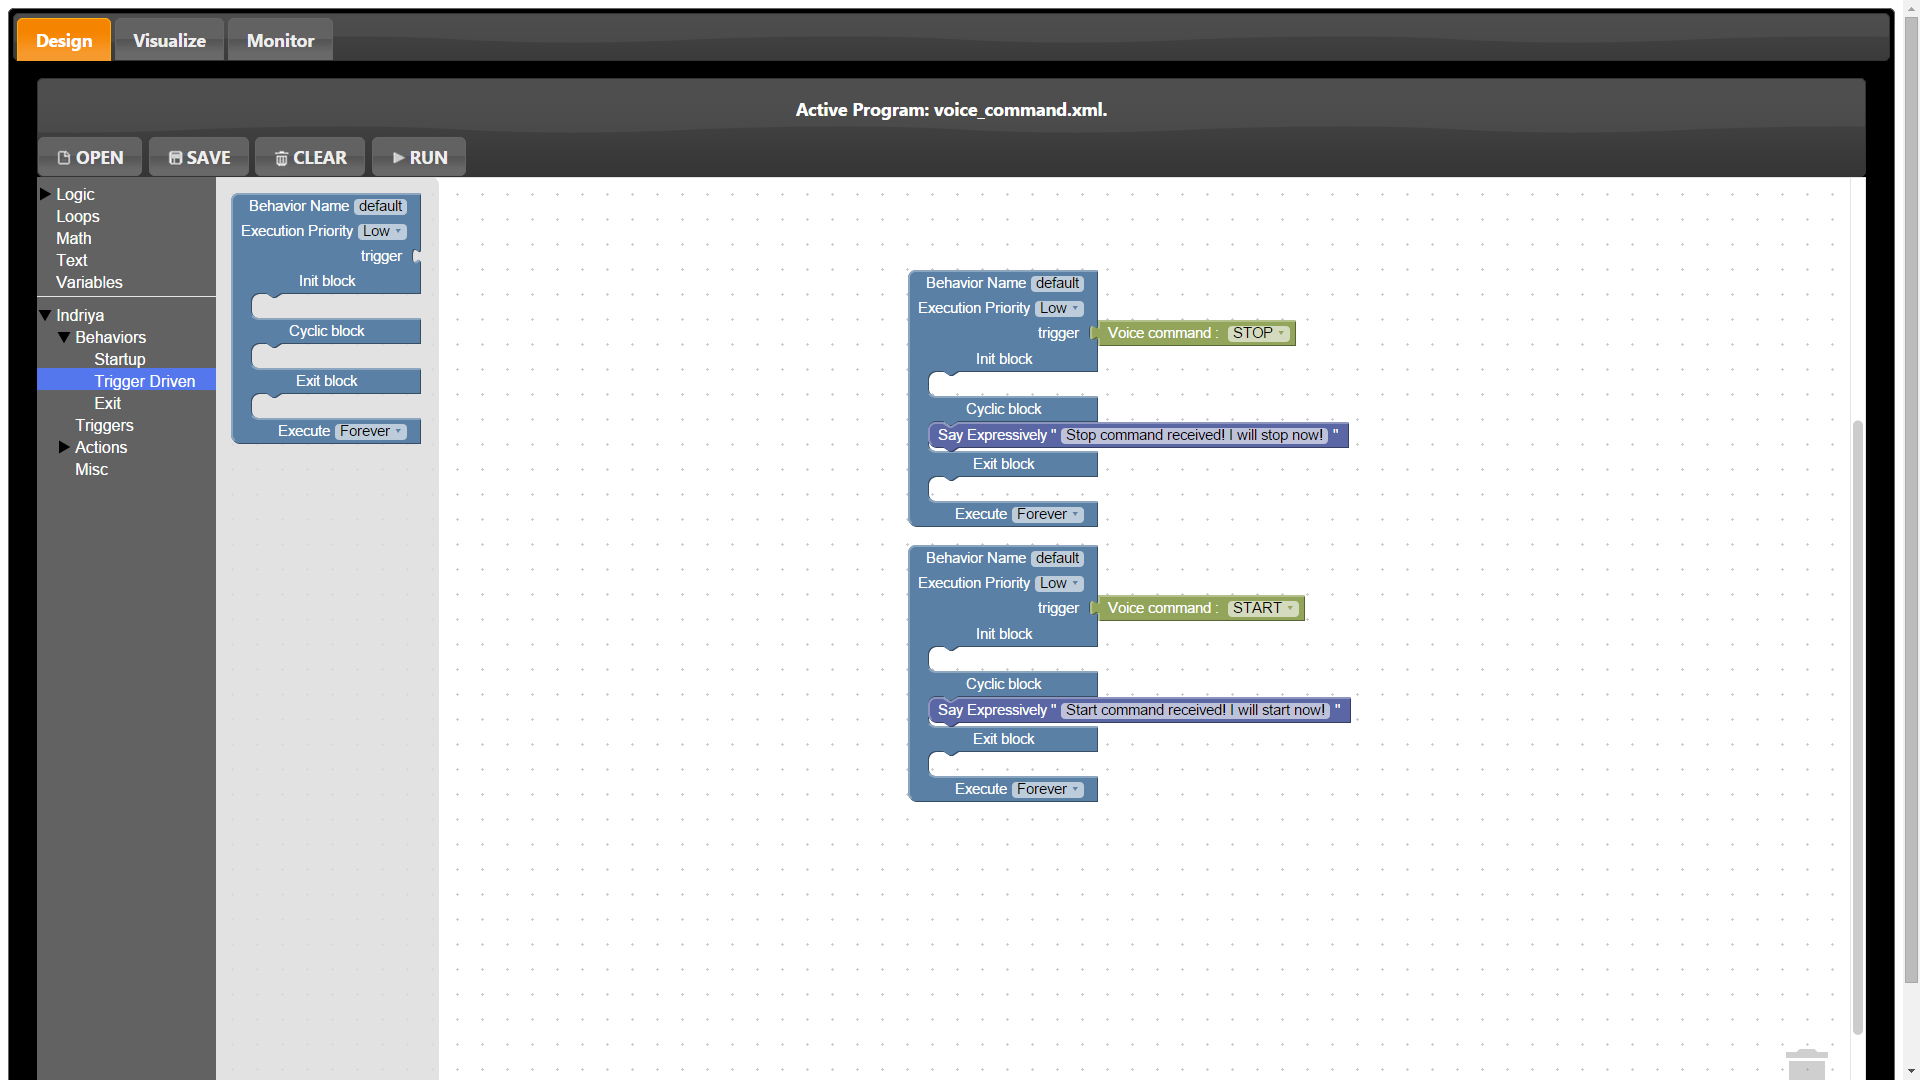
\includegraphics[width=\textwidth]{ui_designer.png}};
    \begin{scope}[x={(image.south east)},y={(image.north west)}]
        %\draw[red,ultra thick,rounded corners] (0.62,0.65) rectangle (0.78,0.75);
        \draw[red,ultra thick,rounded corners] (0,0.93) rectangle (0.22,0.99);
        \draw[red,ultra thick,rounded corners] (0,0.89) rectangle (0.25,0.84);
        \draw[green,ultra thick,rounded corners] (0,0.825) rectangle (0.23,0.01);
        \draw[yellow,ultra thick,rounded corners] (0.4,0.87) rectangle (0.6,0.93);
        \draw[blue,ultra thick,rounded corners] (0.235,0.825) rectangle (0.97,0.01);

        % \draw [-latex, ultra thick, red] (main) to[out=0, in=-120] (0.01,0.96);
        % \draw [-latex, ultra thick, red] (cmd) to[out=0, in=-120] (0.01,0.89);
        % \draw [-latex, ultra thick, green] (toolbox) to[out=0, in=-120] (0.05,0.5);
        % \draw [-latex, ultra thick, yellow] (name) to[out=0, in=-120] (0.5,0.87);
        % \draw [-latex, ultra thick, blue] (surface) to[out=0, in=-120] (0.5,0.5);
        \draw [-stealth, line width=3pt, red] (main) -- ++ (-0.0,-0.15);
        \draw [-stealth, line width=3pt, red] (cmd) -- ++ (-0.12,-0.24);
        \draw [-stealth, line width=3pt, green] (toolbox) -- ++ (0,0.5);
        \draw [-stealth, line width=3pt, yellow] (name) -- ++ (-0.1,-0.19);
        \draw [-stealth, line width=3pt, blue] (surface) -- ++ (0,0.5);
    \end{scope}
\end{tikzpicture}
    \caption[Behavior designer]{Behavior designer}
    \label{fig:behavior_designer}
\end{figure}

The behavior designer is the core component of the user interface. The designer is composed of 
\begin{itemize}
\item Designer command panel : It contains command buttons like Open/Save/Clear/Run which makes it easy to perform operations like creating a new program, saving the program to the server, Clear the workspace and Running the active behavior program
\item Toolbox : It contains behavior, action and trigger blocks needed to realize the behavior program. It also contains the standard logical blocks that comes with Blockly editor.
\item Designer surface: The designer surface is the playground where the user can create behavior program by dropping in blocks from the toolbox.
\end{itemize}

\subsection*{Visualization} The visualization could be used to see the interaction of the human and robot inside a virtual 3D environment.
% Simulation Node
\begin{algorithm}
 \KwData{simulation\_config}
 \textbf{\emph{Init}}:\\
 \quad INIT\_SIMULATION\_ENGINE(simulation\_config) \;
 \quad INIT\_SUBSCRIBERS(simulation\_config) \;
 \quad LOAD\_ENVIRONMENT(simulation\_config) \; 
 \While{True}{
 	sensors = READ\_SENSOR\_VALUES() \; 
 	skeletons = READ\_SKELETON\_DATA() \; 
 	RENDER(robot,sensors)
 }
 %\caption{Localization Algorithm}
 %\label{alg:localize}
\end{algorithm}

\subsection*{Monitor}
The monitor screen shows the current content of the application context in a tree view. This is mainly developed for debugging purpose.

\section{Summary}
 
% Chapter Template

\chapter{System capabilities evaluation} % Main chapter title

\label{Chapter5} % Change X to a consecutive number; for referencing this chapter elsewhere, use \ref{ChapterX}

\lhead{Chapter 5. \emph{System capabilities evaluation}} 

In this chapter various capabilities of Indriya system have been evaluated. The evaluation has been done from a platform developer point of view. The features discussed ranges from intuitiveness to designing complex parallel behaviors on multiple robots. We describe how Indriya system could be used for realistic cases using example programs which would be otherwise extremely difficult to realize using existing methods for a novice programmer.
\section{Indriya: Sensible, intuitive and first of its kind}
In order to describe the simplicity and intuitiveness, we will make a comparative study of a scenario designed with Indriya and with that of Choregraphe behavior design software that comes with NAO humanoid robot. 
\begin{figure}[H]
\centering
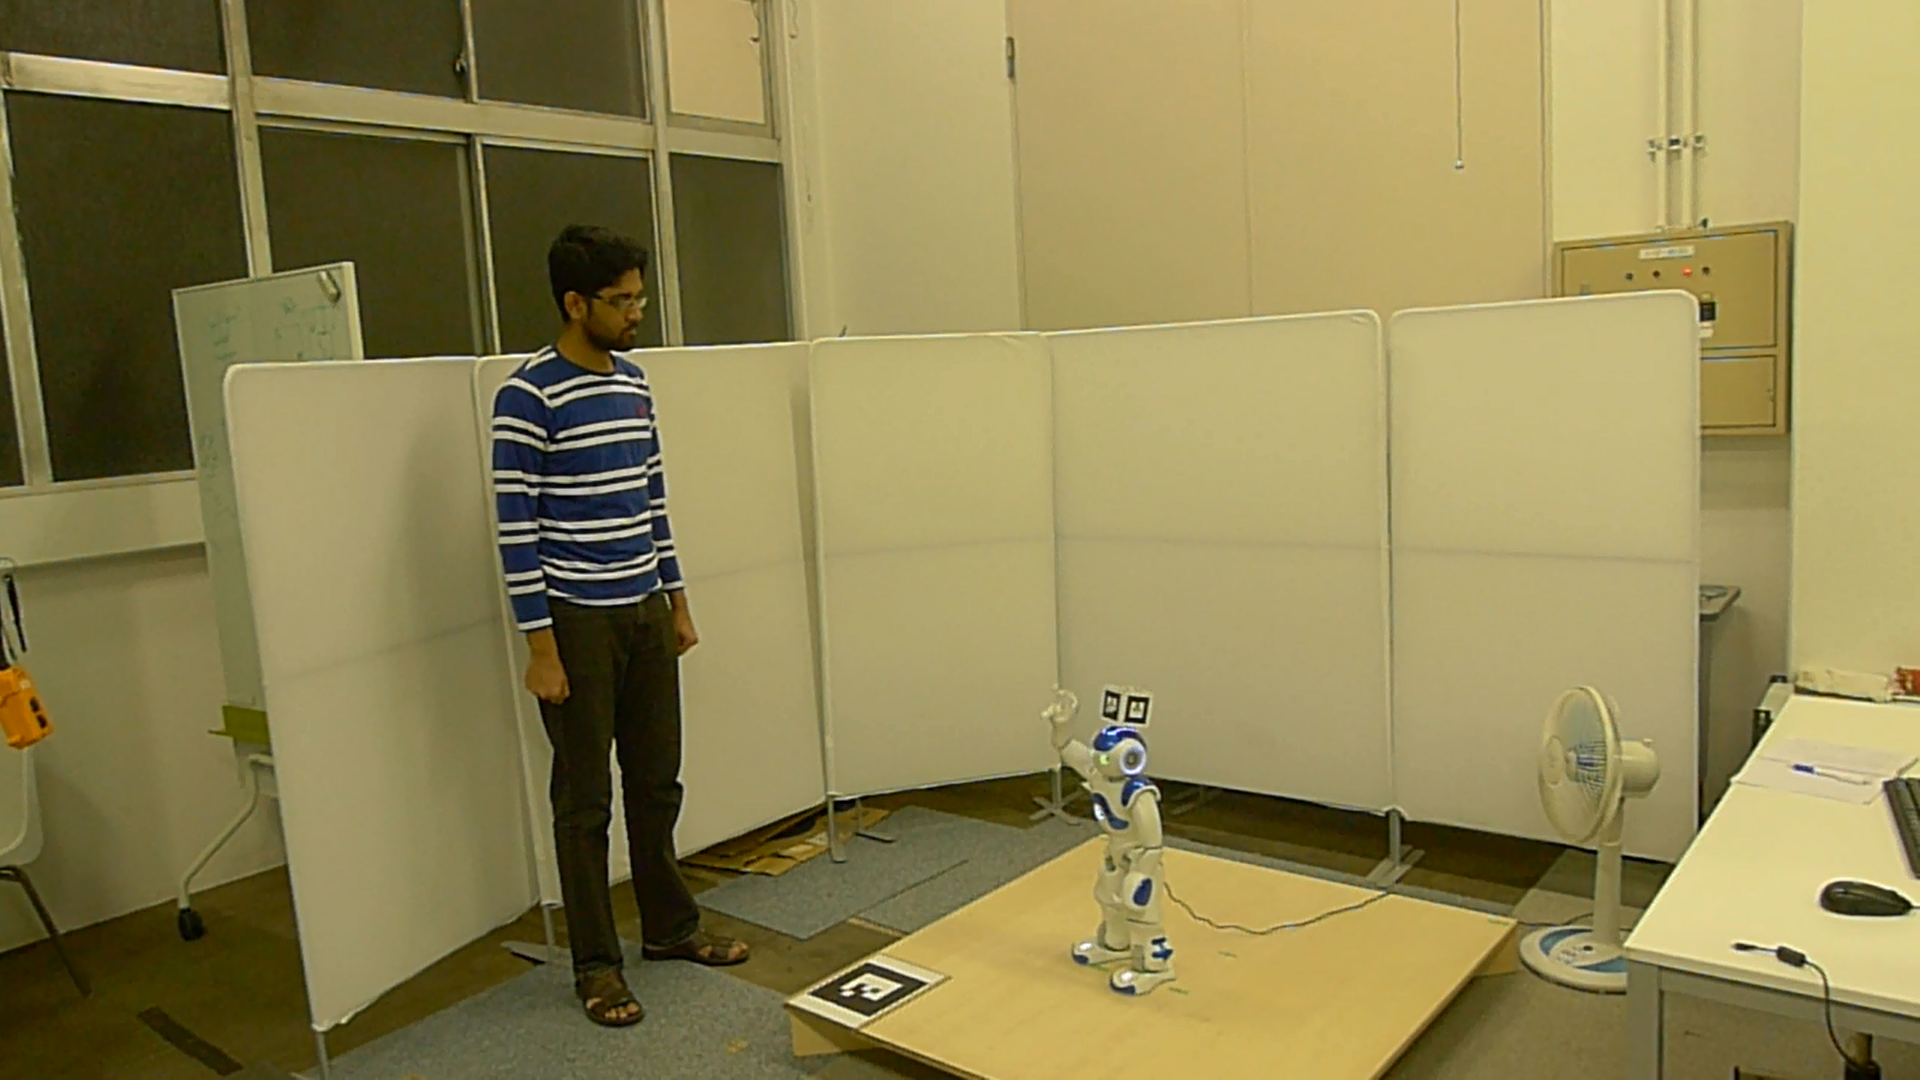
\includegraphics[width=0.8\textwidth]{../thesis/assets/scenario_museum.png}
\caption[NAO museum guide: Experiment setup]{NAO museum guide: Experiment setup}
\label{fig:scenario1_setup}
\end{figure}
\subparagraph{Scenario:}The NAO humanoid robot is a guide in a museum. The museum manager would like to design a scenario where when a visitor comes into the vicinity of the robot, the robot would approach him/her and start explaining the history of the museum. The experiment setup for this scenario is shown in Fig~\ref{fig:scenario1_setup}. We would like to use this scenario to compare the expressiveness and intuitiveness of behavior description with Choregraphe \cite{NaoRobot} shown in Fig~\ref{fig:scenario1_program_choregraphe} and with our interface shown in Fig~\ref{fig:scenario1_program}.
\begin{figure}[H]
\centering
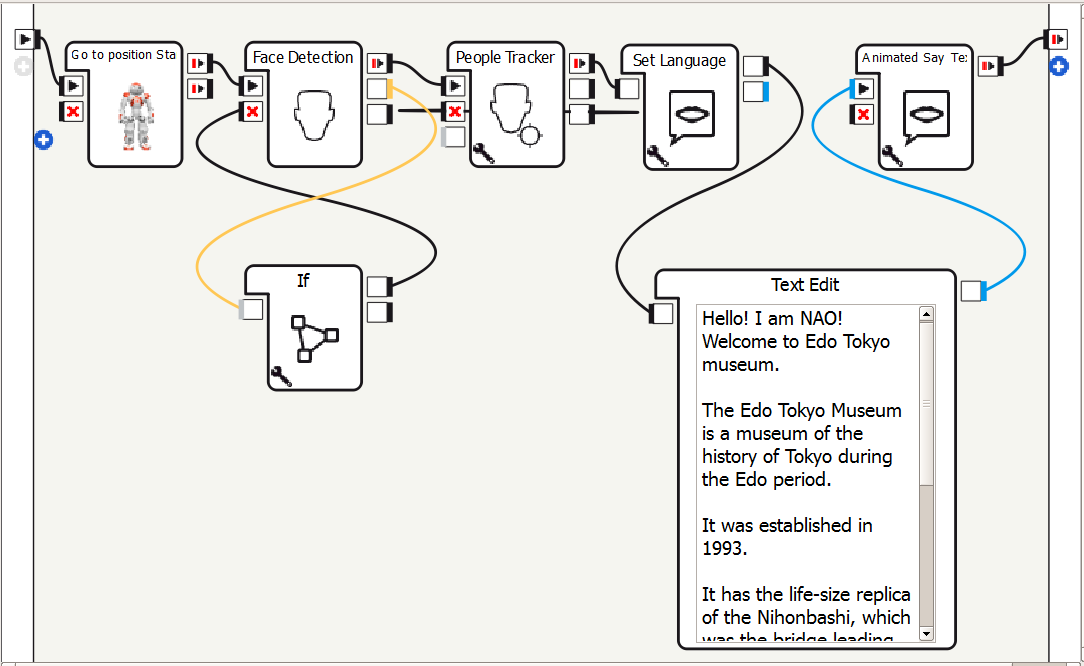
\includegraphics[width=\textwidth]{../thesis/assets/scenario_museum_choregraphe2.png}
\caption[NAO museum guide: Choregraphe Program]{NAO museum guide: Choregraphe Program}
\label{fig:scenario1_program_choregraphe}
\end{figure}
The behavior program desgined using Choregraphe software is shown in Figure~\ref{fig:scenario1_program_choregraphe}. Though Choregraphe uses a familiar flow-chart based programming model and has a huge library of primitive blocks to build complex motion patterns, the data flow for this scenario is not straight forward. As could be noticed from Fig~\ref{fig:scenario1_program_choregraphe}, at first the robot keeps looking for people in its vicinity using the \emph{Face detection block} at the cost of its power. The battery may be used up even before the robot really detects a person. Once it detects a person, the face detection block is stopped and \emph{People tracker} block is activated. The robot starts approaching (tracking) the person until a fixed distance with the person is reached. Once the desired distance of separation is achieved, the people tracker block has to be stopped. Now the robto will actually start explaining the history of the museum. It could be noticed that this kind of description/design of scenario might be easy for a seasoned programmer. However for a novice programmer it could be difficult to think of the dataflow as they literally have to emulate the whole scenario in their mind before designing the system. Moreover for human-in-the-loop scenarios like this, it is extremely difficult to simulate the behavior. So each time the behavior has to be executed in the real robot which increases the overhead of the design process.

Now let us see how such a scenario could be designed using Indriya system. The definition of this scenario is straightforward using Indirya as shown in Fig~\ref{fig:scenario1_program}.
\begin{figure}[H]
\centering
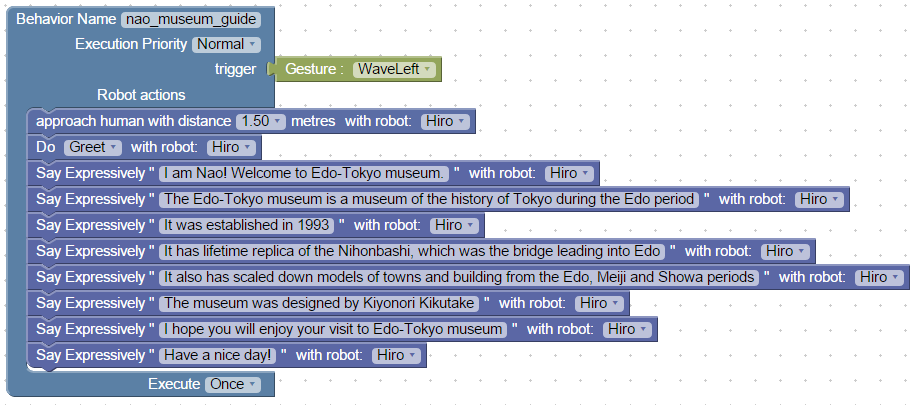
\includegraphics[width=\textwidth]{../thesis/assets/scenario1_new.png}
\caption[NAO museum guide: Indriya Program]{NAO museum guide: Indriya Program}
\label{fig:scenario1_program}
\end{figure}
The framework equipped with Kinect sensor takes care of the detection of people and gives the relative localization of the robot and human. Once the person is detected or a configured gesture trigger arrives, the behavior program retrieves the dynamic position of the robot and of the human from the application context. Using this information, the relative transformation of the human with respect to human is computed. The \emph{Approach block} makes use of this information to drive the robot towards the person. After coming into the proximity of the person, the robot starts explaining the history of museum configured using \emph{Say Expressively} block. From the user perspective, the design of the behavior is \emph{intuitive} using Indriya. He/She can focus on the scenario rather than thinking about the minute details of the data flow as the Indriya system equipped with the perception system acts as a proxy and eases the design process. 
\section{Realistic scenario design}
The Indriya system is not just for toy problems. In this section let us see how it could be used for realistic therapy scenario which is increasingly becoming important for rehabilitation. 
\subparagraph{Scenario:}A physiotherapist who is in a remote hospital would like to prepare an exercise routine for his patient who is recovering from the fracture of his left hand. The therapist wants the service robot in the rehabilitation center to give directions to the patient in an interactive manner and facilitate the process. The exercise is composed of: an introduction and demonstration of the routine, interactively reporting the progress of the exercise and finally notifying the completion. The experiment setup is shown in Figure~\ref{fig:scenario2_setup}
\begin{figure}[H]
\centering
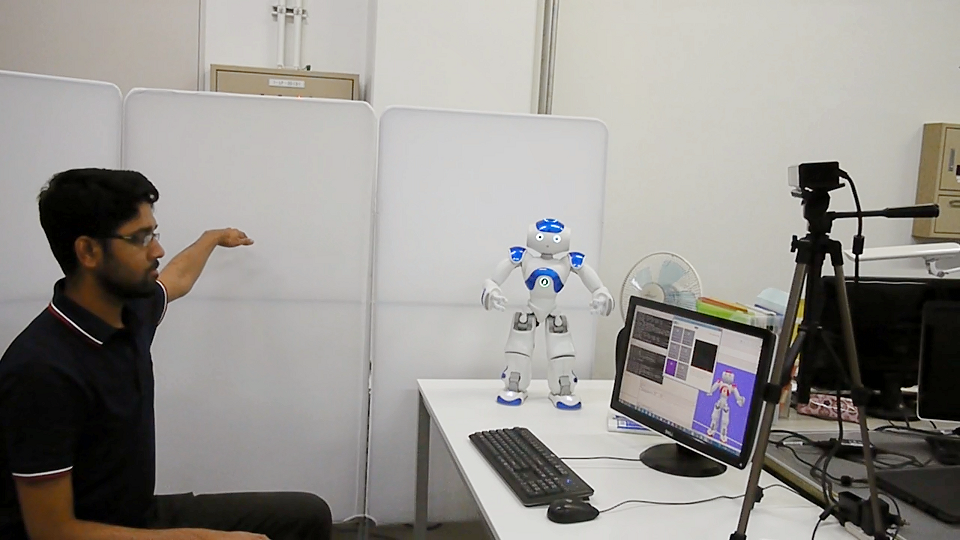
\includegraphics[width=\textwidth]{../thesis/assets/scenario_therapy.png}
\caption[NAO therapy facilitator: Experiment setup]{NAO therapy facilitator: Experiment setup}
\label{fig:scenario2_setup}
\end{figure}
Though Choregraphe software gives the capability of programming behaviors with basic human awareness, it does not explicitly allows programming that takes into account human gestures/motions. This is not the drawback of the system but the fact that it does not enough sensors to understand complex motions. Thanks to the Kinect sensor and its gesture recognition capabilites, one can exploit it to design a program for the above scenario using Indriya system. A reference implementation of such a scenario using our behavior interface is shown in Fig~\ref{fig:scenario2_program}.
\begin{figure}
\centering
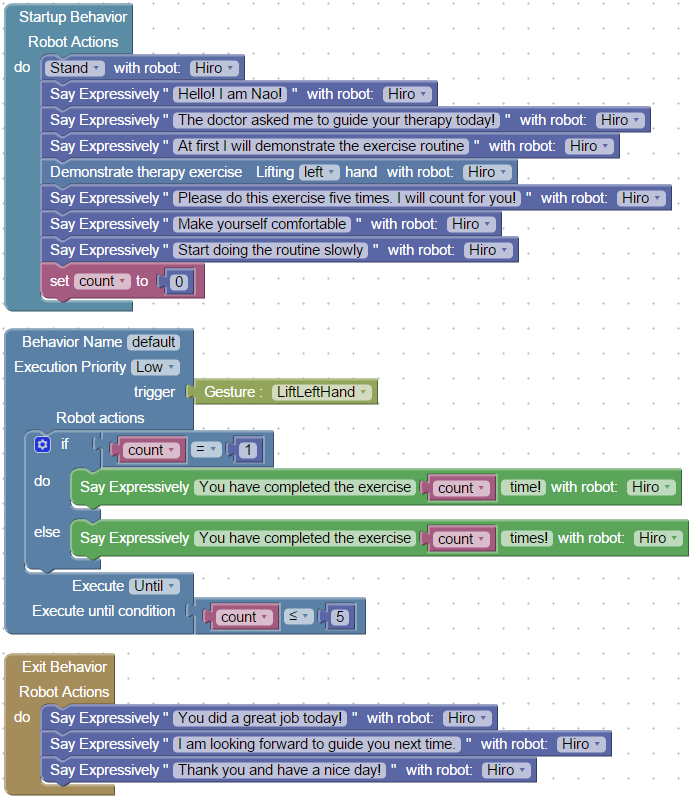
\includegraphics[width=\textwidth]{../thesis/assets/scenario2_new.png}
\caption[NAO therapy facilitator: Indriya program]{NAO therapy facilitator: Indriya program}
\label{fig:scenario2_program}
\end{figure}
The above program is designed using all the three basic behavior constructs that constitutes the behavior program. In the Startup behavior the robot gives an introduction about the exercise routine and then gives a demonstration of how to do it. A trigger behavior block is configured to be triggered each time when the patient performs the therapy routine (lifting left hand). Inside the trigger behavior block in its startup block a variable is initialized to keep track of the count of the triggers. In the cyclic block, the variable is incremented and then the robot notifies the progress of the exercise by announcing how many times the patient has completed the exercise. The trigger behavior block is configured \emph{Until} a desired condition on the exercise count is reached (say lifting left hand 5 times). Once the lifetime of the trigger behavior block expires, the robot gives some closing comments about the routine. It could be noticed that the description of this scenario is quite simple using the Indriya. The blockly editor powered with the behavior program logic abstracts the complexity of designing realistic scenarios.
\section{Multi-robot programming at finger tips}
The Indriya system now supports NAO humanoid robots. It will soon support Turtlebot and Pepper humanoid robot. The main advantage of the system is the robot interface modules developed for each of these robots are designed in such a way that it is easy to create multiple instances (nodes) with the same script by just changing the connection parameters as shown in Listing~\ref{lst:multirobot_config}
\lstinputlisting[caption=Multirobot Configuration File,label={lst:multirobot_config},language=XML]{assets/multirobot_config.xml}
In this way it is easy to extend the system to be used for many robots of same kind and also many different kinds of robots. 
\begin{figure}
\centering
\begin{subfigure}[t]{0.8\textwidth}
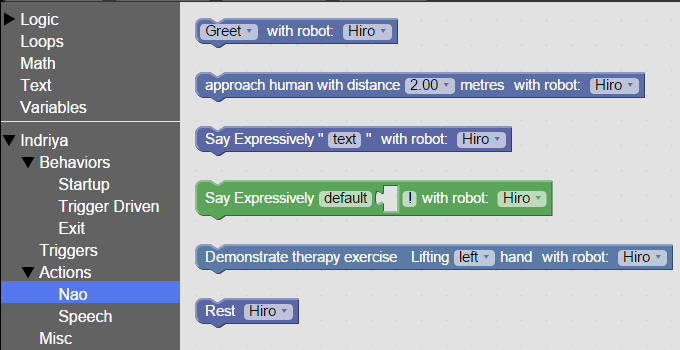
\includegraphics[width=\textwidth]{../thesis/assets/toolbox_multirobot.png}
\caption[Robot categorization]{Robot categorization}
\label{fig:robot_categorize}
\end{subfigure}

\begin{subfigure}[t]{0.8\textwidth}
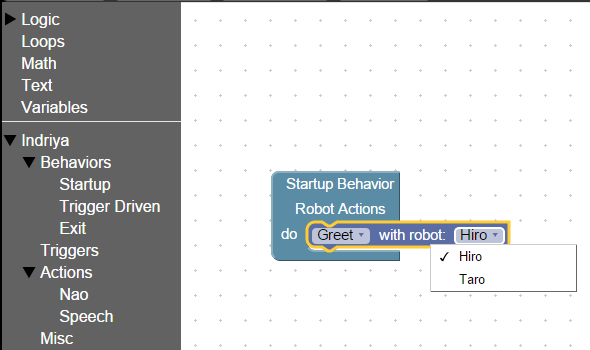
\includegraphics[width=\textwidth]{../thesis/assets/toolbox_multirobot2.png}
\caption[Individual robot selection]{Individual robot selection}
\label{fig:robot_selection}
\end{subfigure}
\caption[Multirobot support]{Multirobot support}
\label{fig:multirobot_support}
\end{figure}
The user interface is also designed in such a way that, it is easy to choose which action to be executed in which robot. The robot actions are categorized by their types in the tool box (Figure~\ref{fig:robot_categorize}) and with the given robot type, for each robot action blocks it is possible to choose the robot by its name (Figure~\ref{fig:robot_selection}) as specified by the user in the configuration file.
A more appropriate scenario for multi-robot interaction scenario is described in Section~\ref{sec:parallel_programming}

\section{Parallel programming: Easier than ever before}
\label{sec:parallel_programming}
Collaborative introduction of Indriya system (2 Nao robots, 3 robots including turtlebot). 

\section{Priority execution making real sense}
Most often in real life HRI scenarios one would like to have robot respond to certain events with a higher priority irrespective of what it is doing at that time. Priority based execution capability comes handy in such scenarios. Priority based execution is inspired from computer processor architectures and scheduling of processes. The inherent problem is that often these concepts are extremely difficult to understand/implement for beginner to intermediate level programmers. The Indriya system makes this extremely easy by just fixing the priority of each behavior blocks. This capability is elucidated in the scenario described below. 

\subparagraph{Scenario:}Let us consider an elderly care robot who takes care of a fictitious person Mr. Adams. The living room is equipped with kinect sensor so that the activities and voice commands of the person could be recognized by Indriya system. The care taker of Mr. Adams who is working during the day would like to design a behavior program for the robot. He/She wants the robot to respond to normal commands like \emph{Come here}, \emph{Bring Coffee} etc., Among others he would like the robot to serve emergency conditions like when the elderly person faint down suddenly, or he/she asks for help due to medical complications etc.,

The reference implementation of the caring robot is shown in Figure~

\section{Summary and Discussion}

Speak about extensiblilty, modularity and software design 
% Chapter Template

\chapter{Behavior Design and Evaluation} % Main chapter title

\label{Chapter6} % Change X to a consecutive number; for referencing this chapter elsewhere, use \ref{ChapterX}

\lhead{Chapter 6. \emph{Behavior Design and Evaluation}} 


\section{Experiment}

\subsection{Protocol}

\subsection{Setup}
\quad The entire framework has been implemented using open network communication standards powered by ZeroMQ \cite{ZeroMQ} and message serialization using the Google's protocol buffers \cite{ProtocolBuffers}. The Kinect for Windows V2 is used as the motion recognition system. A set of gestures are created using the visual gesture builder that comes with Kinect SDK \cite{Kinect2014}. The process involves capturing the motion clips, tagging the clips with the appropriate gestures and training the gesture recognizer. The trained gestures are then exported as a visual gesture database and integrated with the motion recognition node. The humanoid robot NAO H25(V50) powered by the latest NaoQi OS V2.1.3 is used for evaluating the interaction scenarios.  A set of actions of the NAO humanoid robot are developed as python scripts. The localization of the humanoid robot is performed by combining the marker detection using augmented reality toolkit ALVAR \cite{ALVAR} and a simple 2-DOF kinematic model of the robot from torso to the head. The software is tested on a 64-bit Intel Core i7 CPU with clock speed 3.60 Ghz and 8 GB of RAM on a Microsoft Windows 8.1 OS. The source code of the software is available as open source at \url{https://github.com/praveenv4k/ICSORO-2015}
\subsection{Example Scenarios}
\begin{figure}
\centering
\begin{subfigure}[t]{0.49\textwidth}
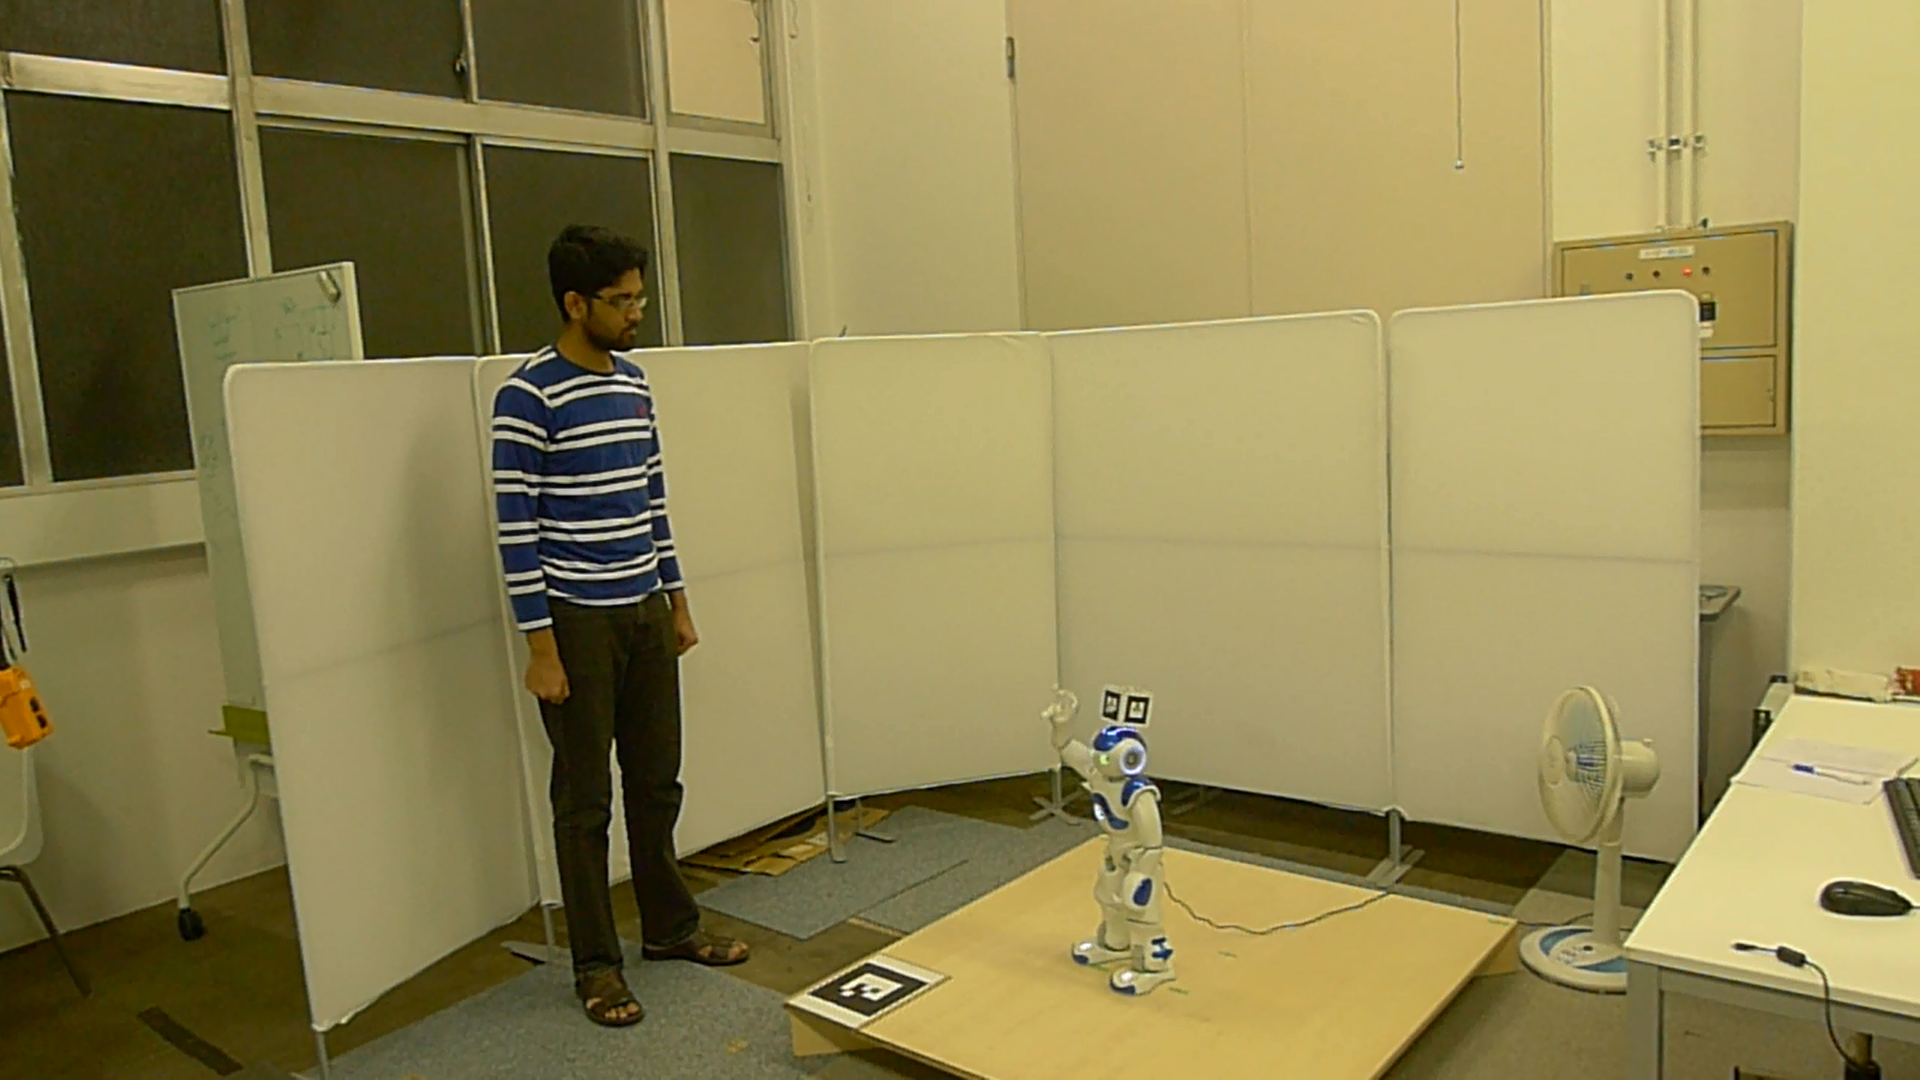
\includegraphics[width=\textwidth]{../thesis/assets/scenario_museum.png}
\caption[Experiment Setup 1]{NAO as museum guide}
\label{fig:scenario1_setup}
\end{subfigure}
\begin{subfigure}[t]{0.49\textwidth}
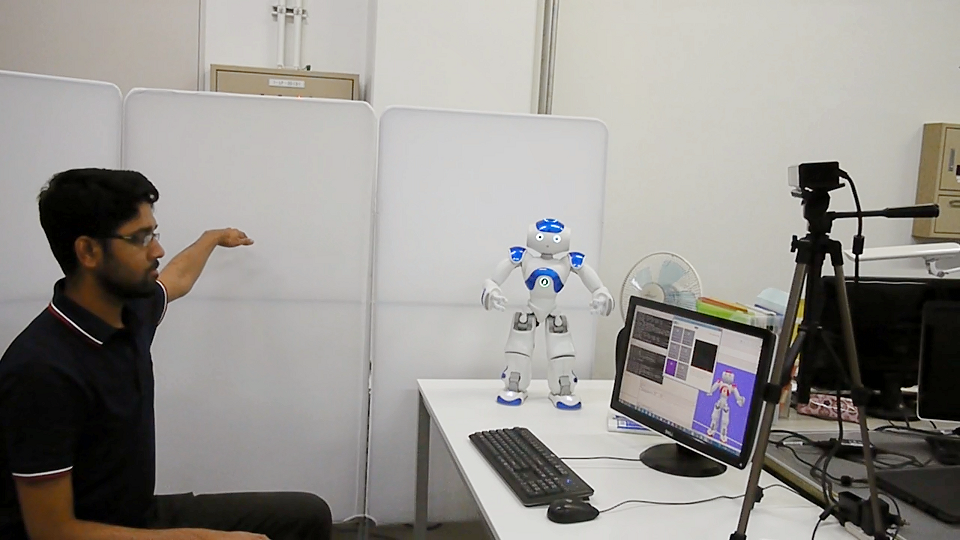
\includegraphics[width=\textwidth]{../thesis/assets/scenario_therapy.png}
\caption[Experiment Setup 2]{NAO as therapy facilitator}
\label{fig:scenario2_setup}
\end{subfigure}
\caption[Experiment Setup]{Experiment Setup}
\label{fig:scenarios_setup}
\end{figure}
	In this section we describe two scenarios to demonstrate how our behavior design system could be used for realistic cases which would be otherwise extremely difficult to realize using existing methods for a novice programmer.
\subsubsection{NAO as museum guide: }
\begin{figure}
\centering
\begin{subfigure}[t]{0.49\textwidth}
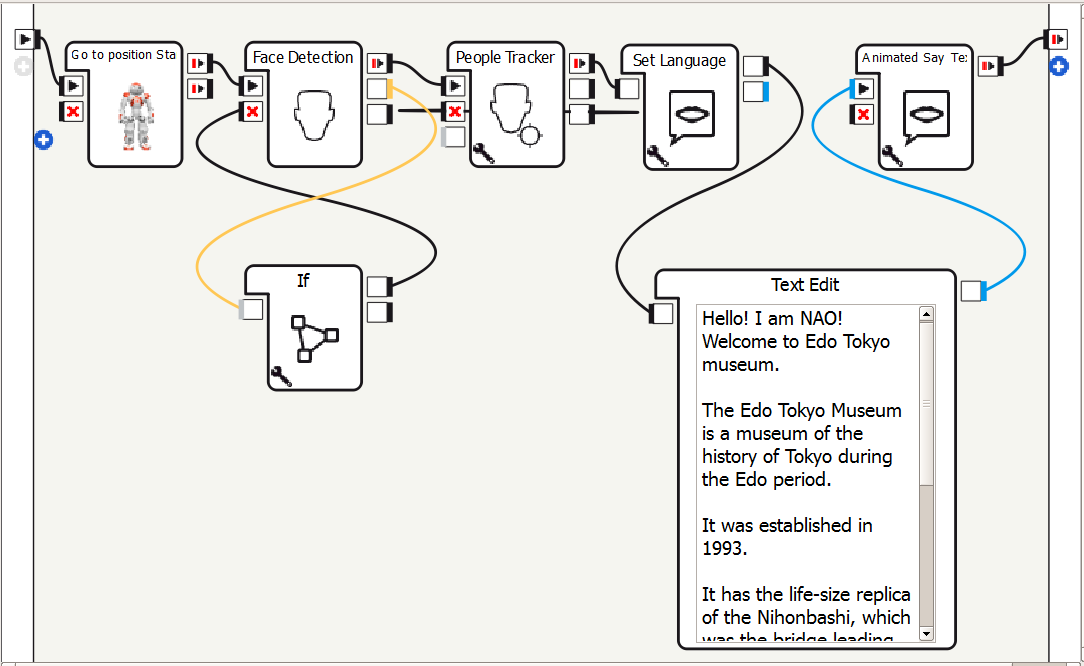
\includegraphics[width=\textwidth]{../thesis/assets/scenario_museum_choregraphe2.png}
\caption[Using Choregraphe]{Using Choregraphe}
\label{fig:scenario1_program_choregraphe}
\end{subfigure}
\begin{subfigure}[t]{0.49\textwidth}
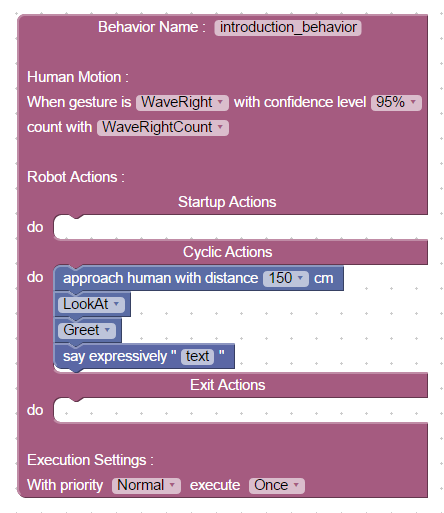
\includegraphics[width=\textwidth]{../thesis/assets/scenario1.png}
\caption[Using our behavior interface]{Using our behavior interface}
\label{fig:scenario1_program}
\end{subfigure}
\caption[NAO as museum guide]{NAO as museum guide}
\label{fig:scenarios}
\end{figure}
	The NAO humanoid robot is a guide in a museum. The museum manager would like to design a scenario where when a visitor comes into the vicinity of the robot, the robot would approach him/her and start explaining the history of the museum. We would like to use this scenario to compare the expressiveness and intuitiveness of behavior description with Choregraphe \cite{NaoRobot} shown in Fig~\ref{fig:scenario1_program_choregraphe} and with our interface shown in Fig~\ref{fig:scenario1_program}.
	
	Though Choregraphe uses a familiar flow-chart based programming model and has a huge library of primitive blocks to build complex motion patterns, the data flow for this scenario is not straight forward. As could be noticed from Fig~\ref{fig:scenario1_program_choregraphe}, at first the robot keeps looking for people in its vicinity at the cost of its power. Once it detects a person, it stops looking for people and start approaching (tracking) the person until a fixed distance with the person is reached. After this the tracking block has to be stopped and now the robot will actually start explaining the history of the museum.
	
	Using our behavior interface, the definition of this scenario is straightforward as shown in Fig~\ref{fig:scenario1_program}. The framework equipped with Kinect sensor takes care of the detection of people and gives the relative localization of the robot and human. Once the person is detected or a configured gesture trigger arrives, the behavior program retrieves the dynamic position of the robot and of the human. Using this information, the robot is driven towards the person. After coming into the proximity of the person, the robot starts explaining the history of museum. From the user perspective, the design of the behavior is intuitive and he/she can just focus on the scenario rather than thinking about the details of the data flow. The experiment setup for this scenario is shown in Fig~\ref{fig:scenario1_setup}.
\subsubsection{NAO as therapy facilitator:}%
\begin{figure}
\includegraphics[width=\textwidth]{../thesis/assets/scenario2_horizontal.png}
\caption[NAO as therapy facilitator]{NAO as therapy facilitator}
\label{fig:scenario2_program}
\end{figure}
A physiotherapist who is in a remote hospital would like to prepare an exercise routine for his patient who is recovering from the fracture of his left hand. The therapist wants the service robot in the rehabilitation center to give directions to the patient in an interactive manner and facilitate the process. The exercise is composed of: an introduction and demonstration of the routine, interactively reporting the progress of the exercise and finally notifying the completion. 
	
This scenario cannot be realized using Choregraphe since it does not explicitly take into account the motion recognition. A reference implementation of such a scenario using our behavior interface is shown in Fig~\ref{fig:scenario2_program}. In the startup behavior an introduction about the exercise routine and a demonstration of the same is performed by the robot. Then each time the patient performs the exercise, the robot notifies the progress of the exercise by announcing how many times the patient has completed the exercise. Once the exercise routine is completed (say lifting left hand 5 times), the robot gives some closing comments about the routine. The experiment setup for this scenario is shown in Fig~\ref{fig:scenario2_setup}. The experiment result of the scenarios are uploaded to \url{http://youtu.be/gdbR199ejrg} 
% Chapter Template

\chapter{Conclusion} % Main chapter title
\label{Chapter7} % Change X to a consecutive number; for referencing this chapter elsewhere, use \ref{ChapterX}
\lhead{Chapter 7. \emph{Conclusion}} 
\section{Project Summary}
In this section summary of the Indriya platform is described
\subsection{System specification}
 The Indriya platform could be seen as a product by itself. The product specification is shown in Table~\ref{table:system_spec}.

\begin{table}[H]
\centering
%\small
\caption{Indriya specification}
\label{table:system_spec}
\begin{tabular}{| p{3.1cm} | p{12cm} |}
\hline
  Hardware & \begin{itemize}[leftmargin=*,topsep={0pt},itemsep={0pt},partopsep={0pt},parsep={0pt}] 
                                                  \item Supported Robots: Nao
                                                  \item Sensor: Kinect for Windows V2
                                                  \item PC: x64 processor, min 4GB memory, Physical dual-core 3.1 GHz or more, USB 3.0 controller, DX11 capable graphics adapter
                                                  \end{itemize} 
                                          \tabularnewline\hline
                                          
  Software &  \begin{itemize}[leftmargin=*,topsep={0pt},itemsep={0pt},partopsep={0pt},parsep={0pt}] 
                                                  \item Platform: Windows 8.1
                                                  \item For running: Microsoft .NET 4.5.1, Visual C++ 2013 redistributable, Naoqi Python SDK v2.3.3, Kinect for Windows SDK
                                                  \item For developing: Please go through readme file: \url{https://github.com/praveenv4k/Indriya/blob/master/README.md}
                                                \end{itemize} 
                                          \tabularnewline\hline
\end{tabular}
\end{table}

In summary Indriya platform
\begin{itemize}
\item Is a software to design HRI scenarios based on human behaviors
\item Gives opportunity to augment multimodal sensor to the existing perception system of the robot
\item Provides easy to user interface for designing the scenarios
\end{itemize}
and it is not
\begin{itemize}
\item A system to design low level control of a robot
\end{itemize}
	
The source code of the complete platform is available as Open source at \url{https://github.com/praveenv4k/Indriya}. 
\subsection{Project Statistics}
The project has an extensive code base consisting of over 30k lines of code (counted using CLOC tool). The software has been written using diverse programming language according to the best fit for the purpose. The code statistics is shown in Fig.\ref{fig:code_stats}.
% \begin{table}[h!]
%   \begin{center}
%     \caption{Project Code Statistics}
%     \label{table:code_stats}
%     \pgfplotstabletypeset[
%       columns = {language,comment,code},
%       multicolumn names, % allows to have multicolumn names
%       col sep=comma, % the seperator in our .csv file
%       %display columns/0/.style={
%       %    column name=$Files$, % name of first column
%       %    column type={S},string type
%       %},  % use siunitx for formatting
%       %display columns/0/.style={
%       %    column name=$Files$,
%       %    string type
%       %},  % use siunitx for formatting
%       display columns/0/.style={
%         column name=$Language$,
%         string type
%       },
%       %display columns/1/.style={
%       %  column name=$Blank$,
%       %  string type
%       %},
%       display columns/1/.style={
%         column name=$Comment$,
%         string type
%       },
%       display columns/2/.style={
%         column name=$Code$,
%         string type
%       },
%       every head row/.style={
%         before row={\toprule}, % have a rule at top
%         after row={
%           %\si{\ampere} & \si{\volt}\\ % the units seperated by &
%           \midrule} % rule under units
%       },
%       every last row/.style={after row=\bottomrule}, % rule at bottom
%     ]{assets/cloc_code_statistics.csv} % filename/path to file
%   \end{center}
% \end{table}

% \begin{figure}[H]
% \centering
% \begin{tikzpicture} 
% \pie[text=legend]{43.85/C\#, 22.83/C++, 9.52/Python, 6.96/Javascript, 16.8/Others} 
% \end{tikzpicture}
% \caption[NAO museum guide: Experiment setup]{NAO museum guide: Experiment setup}
% \label{fig:pie}
% \end{figure}
\begin{figure}[!ht]
  %\centering
  %\rule{6.4cm}{3.6cm}
  \begin{tikzpicture}[scale=0.8]
  %\pie[text=legend]{43.85/C\#, 22.83/C++, 9.52/Python, 6.96/Javascript, 16.8/Others} 
  %\pie[ cloud , text = inside , scale font ]{43.85/C\#, 22.83/C++, 9.52/Python, 6.96/Javascript, 16.8/Others}
  \pie[ cloud , text = inside ]{43.85/C\#, 22.83/C++, 9.52/Python, 6.96/JS, 16.8/Others}
  %\pie[ square]{43.85/C\#, 22.83/C++, 9.52/Python, 6.96/JS, 16.8/Others}
  \end{tikzpicture}
  \qquad
  \begin{tabular}[b]{cc}\hline
    Language & Lines of code \\ \hline
    C\# & 0 \\
    C++ & 0 \\
    Python & 0 \\
    Javascript (JS) & 0 \\
    Others & 0 \\
    Total & 0 \\ \hline
  \end{tabular}
  %\captionlistentry[table]{Indriya: Code statistics}
  %\captionsetup{labelformat=andtable}
  \caption{Indriya: Code statistics}
    \label{fig:code_stats}
\end{figure}

\subsection{Scope for prospective work}
  The Indriya platform has tremendous scope for future developments. Some of the directions that could be thought are

\begin{itemize}
\item Developing a huge database of commonly encountered gestures in social environment
\item Developing an extensive database of robot actions that the user expects it do on a daily basis
\item Developing an interface definition language to generate the visual programming blocks and code generation modules for those blocks automatically.
\item Integration of data management system/user databases to persist and retrieve user information for personalized interaction experience
\item Integration of sensors available in smartphone and wearable devices like IMUs, Gyroscopes, GPS etc.,
\item Integration of Natural Language Processing systems with the speech recognition module for more natural interaction
\item Increasing the range of operation of Humanoid robots by fusing data from two or more Kinect sensors 
\item Support for social behavior learning and intelligence modules for dynamic adoption of human like behavior by robots
\end{itemize}

\section{Conclusion} % Main chapter title
Human Robot Interaction is a complex interdisciplinary problem that needs expertise in various fields like human computer interaction, psychology, sociology, humanoid robotics etc., Social robots have become very common in the recent days and they find useful applications in entertainment, education, autism treatment and elderly care. 

For an efficient interaction with human, the robot has to understand his/her behaviors and also the environment around him. This is only possible when the robot has necessary perception capabilities to make it aware of the situation. However the onboard sensors most often cannot deliver all the information necessary for an effective interaction. The abundance of smart devices and sensors in the smart home and public environments can be exploited for this purpose and RGB-D sensors like Microsoft Kinect provides a convincing solution.

The people from interdisciplinary fields wanting to develop a rich interaction scenario find it difficult to use the existing technology as it requires strong background in programming. Any new programming paradigm designed for such purposes should find a correct balance between simplicity and expressiveness which was the main motivation behind this thesis. The behavior programming paradigm proposed in this thesis could be used for studying various aspects of HRI such as efficiency of the system, cooperativeness, social acceptance etc., There exist some open questions and challenges to be addressed however. The preliminary challenges are to find a set of all possible human motions that could be understood from the sensors distributed around in the environment and to identify all possible actions a robot could perform to interact with human in a social interaction scenario. The next question is to find the spectrum of interaction scenarios this kind of programming interface could cover.  
%% Chapter Template

\chapter{Conclusion} % Main chapter title
\label{Chapter8} % Change X to a consecutive number; for referencing this chapter elsewhere, use \ref{ChapterX}
\lhead{Chapter 8. \emph{Conclusion}} 
	Human Robot Interaction is a complex interdisciplinary problem that needs expertise in various fields like human computer interaction, psychology, biomechanics, humanoid robotics etc., Social robots have become very common in the recent days and they find useful applications in entertainment, education, autism treatment and elderly care. 
	
	For an efficient interaction with human, the robot has to understand his motions and also the environment around him. This is only possible when the robot has necessary perception capabilities which seemlessly make the robot understand the human motions. However the onboard sensors most often cannot deliver all the information necessary for an effective interaction. So there is a need to augment exteroceptive sensors to the system and RGB-D sensors prove to be a convincing solution to this purpose. Irrespective of the underlying perception system used, there is also a need for a scalable robot behavior design framework which could take care of automatic information flow between various components in the system and dynamic creation of behaviors based on object permanence in the environment. Combining the perception system and behavior framework will result in a platform wherein interaction based on human motion will be possible. 
	
	This bibliographic study explained the requirements and challenges in each of the problems of motion understanding, robot localization, behavioral design and evaluation techniques. The state of the art research helped to make appropriate choices to tackle each of the problems under study. More specifically in the research plan described in this study, it is proposed to use Kinect V2 sensor as the perception system and use of Kinect SDK for human motion understanding. The robot localization and tracking problem will be tackled by using a parallelized implementation of particle filter tracking algorithm available in Point cloud library. The Target Drives Means(TDM) framework will be used as the dynamic behavior design infrastructure. An example TDM program is also presented that uses the aforementioned experimental platform. The state of the art HRI evaluation techniques like self assesments and behavioral measures will be used to evaluate the interaction. The experimental platform this thesis aims to achieve will encourage diverse experiments focusing on the evaluation of specific interaction metrics. 
%----------------------------------------------------------------------------------------
%	THESIS CONTENT - APPENDICES
%----------------------------------------------------------------------------------------

\addtocontents{toc}{\vspace{2em}} % Add a gap in the Contents, for aesthetics

\appendix % Cue to tell LaTeX that the following 'chapters' are Appendices

% Include the appendices of the thesis as separate files from the Appendices folder
% Uncomment the lines as you write the Appendices

% Appendix A

\chapter{Statistical Tools} % Main appendix title
\label{AppendixA} % For referencing this appendix elsewhere, use \ref{AppendixA}
\lhead{Appendix A. \emph{Statistical Tools}} % This is for the header on each page - perhaps a shortened title
	A summary of the most commonly used statistical tools in HRI are presented below.
\begin{enumerate}
\item \emph{Mean, Variance} The most simplest way of statistical analysis of a set of data is to represent them with their mean and the standard deviation. Let $X$ be the set of data collected with $X_i$ being the result of the $i^{th}$ experiment $(i = 1..N)$, the mean $\mu_X$ and the standard deviation $\sigma_X$ are given by
\begin{align*}
\mu_X    &= \frac{1}{N} \sum_{i=1}^{N} X_i\ ; \quad \sigma_X = \sqrt{\frac{1}{N} \sum_{i=1}^{N} (X_i - \mu_X)^2}
\end{align*}
Additionally more often the variability of the data in the set is express by the variance ${\sigma_X}^2$. Suppose we consider another set of data $Y$ characterized by its mean $\mu_Y$ and standard deviation $\sigma_Y$, more often in the statistical analysis we will be coming across cases in which the observations in the set $X$ will be related to the observations in the set $Y$. The \emph{covariance (cov(X,Y))} gives the measure of how to the observations in sets $X,Y$ change together and is given by
\begin{align*}
cov(X,Y) = \frac{1}{N} \sum_{i=1}^{N} (X_i - \mu_X) (Y_i - \mu_Y) 
\end{align*}
\item \emph{Pearson Correlation Coefficient (PCC)} : Pearson’s correlation coefficient is a statistical measure of the strength of a linear relationship between paired data. In a sample it is denoted by $\rho$ and is by design constrained as: $-1 \leq \rho \leq 1$. Positive values indicate positive linear correlation, negative values indicate negative linear correlation and a value of 0 indicate no correlation. PCC is given by
\begin{equation}
\rho_{X,Y} = \frac{cov(X,Y)}{\sigma_X\sigma_Y} \\
% = \frac{E[(X-\mu_X)(Y-\mu_Y)]}{\sigma_X\sigma_Y}
\end{equation}
\item \emph{Spearman Correlation Coefficient (SCC)} : SCC is defined as the PCC between ranked variables. For a sample size of $n$, the $n$ raw scores $X_i,Y_i$ are converted to ranks $x_i,y_i$ and $\rho_s$ is computed as
\begin{equation}
\rho_s = 1-\frac{6\sum {d_i}^2}{n(n^2-1)} 
\end{equation}
where $d_i=x_i-y_i$ is the difference between the ranks. If the raw scores have equal values then identical values are assigned to them as the average of their ranks. The SPCC is less sensitive than the Pearson correlation to strong outliers. 
\item \emph{T-test} : T-test could be used for comparing the means of two set of samples, even if they have different numbers of replicates. In simple terms, the t-test compares the actual difference between two means in relation to the variation in the data (expressed as the standard deviation of the difference between the means). The \emph{One-sample t-test} where in to test the null hypothesis for a set $X:(N,\mu_X,\sigma_X)$ that the sample mean $\mu_X$ is equal to $\mu_0$ one case use
\begin{align*}
t = \frac{\mu_X - \mu_0}{\sigma_X/\sqrt{N}}
\end{align*}
The degree of freedom used for this case is $N=1$. Alternatively a more general form of \emph{Paired t-test} for the two sets $X:(N1,\mu_X,\sigma_X),\ Y:(N2,\mu_Y,\sigma_Y)$ where unequal variances and samples sizes are assumed is given by \emph{Welch's t-test}. The t- statistic to test whether the means are different is given for this case by
\begin{align*}
t &= \frac{\mu_X-\mu_Y}{\sigma_{\mu_X-\mu_Y}} \quad \text{where} \quad \sigma_{\mu_X-\mu_Y} = \sqrt{\frac{{\sigma_X}^2}{N1}+\frac{{\sigma_Y}^2}{N2}} 
\end{align*}
\item \emph{Analysis of Variance (ANOVA)} : ANOVA uses a single hypothesis test to check whether the means across many groups are equal. In simple terms, ANOVA generalizes t-test to more than two sets.  
%\item \emph{Chi-Test}
\item \emph{Cronbach's alpha} : Cronbach's $\alpha$ is used as a lowerbound estimate of the reliability of a psychometric test. Suppose that we measure a quantity which is a sum of $N$ components $X = \sum_{i=1}^{N} Y_i$, Cronbach's $\alpha$ is defined as 
\begin{align*}
\alpha = \frac{N}{N-1} (1 - \frac{\sum_{i=1}^{N} {\sigma_{Y_i}}^2}{{\sigma_{X}}^2})
\end{align*}
where ${\sigma_X}^2,{\sigma_{Y_i}}^2$ are the variances of total test scores and that of $i^{th}$ test score respectively. Cronbach's alpha will generally increase as the intercorrelations among test items increase, and is thus known as an internal consistency estimate of reliability of test scores.
\end{enumerate}

%% Appendix Template

\chapter{Rigid Body Transformation} % Main appendix title

\label{AppendixB} % Change X to a consecutive letter; for referencing this appendix elsewhere, use \ref{AppendixX}

\lhead{Appendix B. \emph{Rigid Body Transformation}} % Change X to a consecutive letter; this is for the header on each page - perhaps a shortened title

	\emph{Rigid body} is the one in which distance between any two given points on it remains constant in time regardless of external forces exerted on it. Rigid body transformation forms the basic components in the pose detection framework. In this appendix we give the key ideas behind the rigid body transformations. We consider a $3D$ operational space represented by the vector space $\Re^3$. We consider a right-handed reference frame with homogenous dimensions along each axes. In $\Re^3$, a rigid body is represented by \emph{6 degrees of freedom (DOF)}, 3 for the position along each of the coordinate axes (cartesian coordinates) $P = [p_x,p_y,p_z]^{\text{T}}$ and 3 for the orientation $R$. Considering the system shown in the Figure~\ref{fig:frame_ref} below where $F_0$ is the world frame and $F_1$ is the frame attached to the rigid body. Suppose we know the position $^{1}P$ in the frame $F_1$ and let $^{0}O_1$ be the relative displacement of $F_1$ with respect to $F_0$. Given this framework, the position $^{0}P$ can be given by using the \emph{Homogenous Transformation Matrix}: $^{0}T_1$.
	
\begin{wrapfigure}{r}{0.5\textwidth}
\begin{center}
\includegraphics[width=0.5\textwidth]{assets/rigid_body.png}
\end{center}
\caption{Rigid body transformation}
\label{fig:frame_ref}
\end{wrapfigure}

\begin{align*}
^{0}T_1 = \begin{bmatrix}
^{0}R_1 & ^{0}O_1 \\
0_{1\times 3} & 1
\end{bmatrix}
=
\begin{bmatrix}
n_x & s_x & a_x & o_x \\
n_y & s_y & a_y & o_y \\
n_z & s_z & a_z & o_z \\
0 & 0 & 0 & 1 \\
\end{bmatrix}
\end{align*}


where $^{0}R_1$ is the direction cosine matrix describing the rotation of the frame $F_1$ with respect to $F_0$. $^{0}R_1$ is an orthonormal matrix so ideally 3-DOF is enough for the representation of the orientation. A quick look of the different representation of orientation is presented in Table~\ref{table:rotation} 

\begin{table}

\end{table}
%% Appendix Template

\chapter{Message API} % Main appendix title

\label{AppendixC} % Change X to a consecutive letter; for referencing this appendix elsewhere, use \ref{AppendixX}

\lhead{Appendix C. \emph{Platform Message API}} % Change X to a consecutive letter; this is for the header on each page - perhaps a shortened title

The message are describes using the Google Protocol buffer format and the message definitions are stored in the \emph{proto} files which will be consumed by the code generators to generate the code in the desired programming language (one of C++, Python, Java, C\#). Although some of the primitive message definitions are imported from the Gazebo framework (which also uses Protocol buffers for message serialization), a lot of custom message types are defined for the Indriya framework. The Message API is listed in this Appendix.
\section{Message Type}\label{protocol-documentation}
\subsection{Gesture}\label{gesture.proto}
\subsubsection*{GestureDescription} Represents a gesture description
\begin{longtable}[l]{@{}llll@{}}
\toprule
Field & Type & Label & Description\tabularnewline
\midrule
\endhead
name & string & required & Name of the gesture\tabularnewline
type & GestureDescription.GestureType & required & Type of
gesture/motion\tabularnewline
active & bool & optional & Active status of gesture\tabularnewline
progress & int32 & optional & Gesture progress\tabularnewline
confidence & int32 & optional & Gesture recognition
confidence\tabularnewline
\bottomrule
\end{longtable}
\subsubsection*{GestureRecognitionModule} Represents a gesture recognition module
\begin{longtable}[l]{@{}llll@{}}
\toprule
Field & Type & Label & Description\tabularnewline
\midrule
\endhead
name & string & required & Module name\tabularnewline
params & Param & repeated & Module parameters\tabularnewline
motions & GestureDescription & repeated & List of gestures recognition
capabilities of this module\tabularnewline
\bottomrule
\end{longtable}
 \subsubsection*{GestureRecognitionModules} Represents a gesture recognition modules
\begin{longtable}[l]{@{}llll@{}}
\toprule
Field & Type & Label & Description\tabularnewline
\midrule
\endhead
modules & GestureRecognitionModule & repeated & Gesture recognition
module list\tabularnewline
\bottomrule
\end{longtable}
 \subsubsection*{GestureTrigger} Represents a gesture trigger
\begin{longtable}[l]{@{}llll@{}}
\toprule
Field & Type & Label & Description\tabularnewline
\midrule
\endhead
id & int32 & required & Trigger Identifier\tabularnewline
motion & GestureDescription & required & Recognized
gesture\tabularnewline
\bottomrule
\end{longtable}
\subsubsection*{GestureTriggers} Represents a list of gesture trigger
\begin{longtable}[l]{@{}llll@{}}
\toprule
Field & Type & Label & Description\tabularnewline
\midrule
\endhead
id & int32 & required & Identifier\tabularnewline
motion & GestureDescription & repeated & Recognized
gestures\tabularnewline
\bottomrule
\end{longtable}
 \subsubsection*{GestureDescription.GestureType} Represents gesture type
\begin{longtable}[l]{@{}lll@{}}
\toprule
Name & Number & Description\tabularnewline
\midrule
\endhead
None & 0 & No gesture\tabularnewline
Discrete & 1 & Discrete gesture\tabularnewline
Continuous & 2 & Continuous gesture\tabularnewline
\bottomrule
\end{longtable}
\subsection{Human}\label{human.proto}
\subsubsection*{Human} Represents information about a human
\begin{longtable}[l]{@{}llll@{}}
\toprule
Field & Type & Label & Description\tabularnewline
\midrule
\endhead
id & int32 & required & Unique identifier\tabularnewline
tracked & bool & required & True if tracked\tabularnewline
torso\_position & Vector3d & required & Position the
torso\tabularnewline
head\_position & Vector3d & required & Position of the
head\tabularnewline
orientation & Quaternion & required & Torso orientation\tabularnewline
\bottomrule
\end{longtable}
\subsubsection*{Humans} Represents a list of human
\begin{longtable}[l]{@{}llll@{}}
\toprule
Field & Type & Label & Description\tabularnewline
\midrule
\endhead
human & Human & repeated & List of human\tabularnewline
\bottomrule
\end{longtable}
\subsection{Joint Value}\label{jointux5fvalueux5fmap.proto}
\subsubsection*{JointValue} Represents the Joint value.
\begin{longtable}[l]{@{}llll@{}}
\toprule
Field & Type & Label & Description\tabularnewline
\midrule
\endhead
id & int32 & required & Joint Identifier\tabularnewline
value & double & required & Joint value\tabularnewline
\bottomrule
\end{longtable}
\subsubsection*{JointValueVector} Represents the list of joint values.
\begin{longtable}[l]{@{}llll@{}}
\toprule
Field & Type & Label & Description\tabularnewline
\midrule
\endhead
JointValues & JointValue & repeated & List of joints\tabularnewline
\bottomrule
\end{longtable}
\subsection{Kinect Body}\label{kinectux5fbody.proto}
\subsubsection*{KinectBodies} Represents a list of kinect body
\begin{longtable}[l]{@{}llll@{}}
\toprule
Field & Type & Label & Description\tabularnewline
\midrule
\endhead
Body & KinectBody & repeated & List of kinect bodies\tabularnewline
\bottomrule
\end{longtable}
\subsubsection*{KinectBody} Represents a body
\begin{longtable}[l]{@{}llll@{}}
\toprule
Field & Type & Label & Description\tabularnewline
\midrule
\endhead
TrackingId & int32 & required & Human Tracking Identifier\tabularnewline
IsTracked & bool & required & True if skeleton tracked\tabularnewline
JointCount & int32 & required & Number of joints in the
skeletoon\tabularnewline
Joints & KinectJoint & repeated & List of joints\tabularnewline
ClippedEdges & KinectBody.FrameEdges & optional & Occluded
edge\tabularnewline
HandLeftConfidence & KinectBody.TrackingConfidence & optional & Left
hand tracking confidence\tabularnewline
HandLeftState & KinectBody.HandState & optional & Left hand state
(open/closed/lasso)\tabularnewline
HandRightConfidence & KinectBody.TrackingConfidence & optional & Right
hand tracking confidence\tabularnewline
HandRightState & KinectBody.HandState & optional & Right hand state
(open/closed/lasso)\tabularnewline
IsRestricted & bool & optional & Restricted skeleton\tabularnewline
Lean & Vector2d & optional & Lean point\tabularnewline
LeanTrackingState & int32 & optional & Lean tracking
state\tabularnewline
\bottomrule
\end{longtable}
\subsubsection*{KinectBody.Activity} Represents human engagement
\begin{longtable}[l]{@{}lll@{}}
\toprule
Name & Number & Description\tabularnewline
\midrule
\endhead
EyeLeftClosed & 0 & Left eye closed.\tabularnewline
EyeRightClosed & 1 & Right eye closed.\tabularnewline
MouthOpen & 2 & Mouth open.\tabularnewline
MouthMoved & 3 & Mouth moved.\tabularnewline
LookingAway & 4 & Looking away.\tabularnewline
\bottomrule
\end{longtable}
\subsubsection*{KinectBody.Appearance} Represents the appearance of the human
\begin{longtable}[l]{@{}lll@{}}
\toprule
Name & Number & Description\tabularnewline
\midrule
\endhead
WearingGlasses & 0 & Wearing glasses.\tabularnewline
\bottomrule
\end{longtable}
\subsubsection*{KinectBody.DetectionResult} Represents the gesture recognition result
\begin{longtable}[l]{@{}lll@{}}
\toprule
Name & Number & Description\tabularnewline
\midrule
\endhead
Unknown & 0 & Undetermined detection.\tabularnewline
No & 1 & Not detected.\tabularnewline
Maybe & 2 & Maybe detected.\tabularnewline
Yes & 3 & Is detected.\tabularnewline
\bottomrule
\end{longtable}
\subsubsection*{KinectBody.Expression} The expression a body may have.
\begin{longtable}[l]{@{}lll@{}}
\toprule
Name & Number & Description\tabularnewline
\midrule
\endhead
Neutral & 0 & Neutral expression.\tabularnewline
Happy & 1 & Happy expression.\tabularnewline
\bottomrule
\end{longtable}
\subsubsection*{KinectBody.FrameEdges} Possible occlusion edges
\begin{longtable}[l]{@{}lll@{}}
\toprule
Name & Number & Description\tabularnewline
\midrule
\endhead
None & 0 & No frame edges.\tabularnewline
Right & 1 & Right frame edge.\tabularnewline
Left & 2 & Left frame edge.\tabularnewline
Top & 4 & Top frame edge.\tabularnewline
Bottom & 8 & Bottom frame edge.\tabularnewline
\bottomrule
\end{longtable}
\subsubsection*{KinectBody.HandState} The state of a hand of a body.
\begin{longtable}[l]{@{}lll@{}}
\toprule
Name & Number & Description\tabularnewline
\midrule
\endhead
HS\_Unknown & 0 & Undetermined hand state.\tabularnewline
HS\_NotTracked & 1 & Hand not tracked.\tabularnewline
HS\_Open & 2 & Open hand.\tabularnewline
HS\_Closed & 3 & Closed hand.\tabularnewline
HS\_Lasso & 4 & Lasso (pointer) hand.\tabularnewline
\bottomrule
\end{longtable}
\subsubsection*{KinectBody.TrackingConfidence} Represents tracking confidence
\begin{longtable}[l]{@{}lll@{}}
\toprule
Name & Number & Description\tabularnewline
\midrule
\endhead
Low & 0 & Low confidence.\tabularnewline
High & 1 & High confidence.\tabularnewline
\bottomrule
\end{longtable}
\subsection{Kinect Joint}\label{kinectux5fjoint.proto}
\subsubsection*{KinectJoint} Represents the Kinect skeleton joint data.
\begin{longtable}[l]{@{}llll@{}}
\toprule
Field & Type & Label & Description\tabularnewline
\midrule
\endhead
Type & KinectJoint.JointType & required & Type of skeleton
joint\tabularnewline
State & KinectJoint.TrackingState & required & Tracking state of the
joint\tabularnewline
Position & Vector3d & required & 3D position of the joint\tabularnewline
Orientation & Quaternion & required & 3D orientation of the
joint\tabularnewline
Angle & float & optional & Angle at the joint\tabularnewline
\bottomrule
\end{longtable}
\subsubsection*{KinectJoint.JointType} Represents the types of joints of a Body.
\begin{longtable}[l]{@{}lll@{}}
\toprule
Name & Number & Description\tabularnewline
\midrule
\endhead
SpineBase & 0 & Base of the spine.\tabularnewline
SpineMid & 1 & Middle of the spine.\tabularnewline
Neck & 2 & Neck.\tabularnewline
Head & 3 & Head.\tabularnewline
ShoulderLeft & 4 & Left shoulder.\tabularnewline
ElbowLeft & 5 & Left elbow.\tabularnewline
WristLeft & 6 & Left wrist.\tabularnewline
HandLeft & 7 & Left hand.\tabularnewline
ShoulderRight & 8 & Right shoulder.\tabularnewline
ElbowRight & 9 & Right elbow.\tabularnewline
WristRight & 10 & Right wrist.\tabularnewline
HandRight & 11 & Right hand.\tabularnewline
HipLeft & 12 & Left hip.\tabularnewline
KneeLeft & 13 & Left knee.\tabularnewline
AnkleLeft & 14 & Left ankle.\tabularnewline
FootLeft & 15 & Left foot.\tabularnewline
HipRight & 16 & Right hip.\tabularnewline
KneeRight & 17 & Right knee.\tabularnewline
AnkleRight & 18 & Right ankle.\tabularnewline
FootRight & 19 & Right foot.\tabularnewline
SpineShoulder & 20 & Between the shoulders on the spine.\tabularnewline
HandTipLeft & 21 & Tip of the left hand.\tabularnewline
ThumbLeft & 22 & Left thumb.\tabularnewline
HandTipRight & 23 & Tip of the right hand.\tabularnewline
ThumbRight & 24 & Right thumb.\tabularnewline
\bottomrule
\end{longtable}
\subsubsection*{KinectJoint.TrackingState} Represents the skeleton joint tracking state.
\begin{longtable}[l]{@{}lll@{}}
\toprule
Name & Number & Description\tabularnewline
\midrule
\endhead
NotTracked & 0 & / The joint data is not tracked and no data is known
about this joint.\tabularnewline
Inferred & 1 & / The joint data is inferred and confidence in the
position data is lower than\tabularnewline
Tracked & 2 & / if it were Tracked./ The joint data is being tracked and
the data can be trusted.\tabularnewline
\bottomrule
\end{longtable}
\subsection{Node}\label{node.proto}
\subsubsection*{Node} Represents information of a distributed node
\begin{longtable}[l]{@{}llll@{}}
\toprule
Field & Type & Label & Description\tabularnewline
\midrule
\endhead
name & string & required & Name of the node\tabularnewline
param & Param & repeated & Node parameters\tabularnewline
publisher & Publish & repeated & List of message
publishers\tabularnewline
subscriber & Subscribe & repeated & List of message
subscribers\tabularnewline
\bottomrule
\end{longtable}
\subsection{Param}\label{param.proto}
\subsubsection*{Param} Represents the Parameter Data.
\begin{longtable}[l]{@{}llll@{}}
\toprule
Field & Type & Label & Description\tabularnewline
\midrule
\endhead
key & string & required & Unique key (identifier) of the
parameter\tabularnewline
value & string & required & Parameter value\tabularnewline
dataType & string & required & Parameter Datatype (one of bool, int,
double, string, csv, file)\tabularnewline
\bottomrule
\end{longtable}
\subsubsection*{ParamList} Represents the list of Parameters.
\begin{longtable}[l]{@{}llll@{}}
\toprule
Field & Type & Label & Description\tabularnewline
\midrule
\endhead
param & Param & repeated &\tabularnewline
\bottomrule
\end{longtable}
\subsection{Publisher}\label{publish.proto}
\subsubsection*{Publish} Represents a message publisher
\begin{longtable}[l]{@{}llll@{}}
\toprule
Field & Type & Label & Description\tabularnewline
\midrule
\endhead
topic & string & required & Publisher topic\tabularnewline
msg\_type & string & required & Message type\tabularnewline
host & string & required & Host address\tabularnewline
port & uint32 & required & Host port\tabularnewline
\bottomrule
\end{longtable}
\subsection{Quaternion}\label{quaternion.proto}
\subsubsection*{Quaternion} Represents a Quaternion (axis,angle) =\textgreater{}(w = cos(angle/2), {[}x,y,z{]} = axis* sin(angle/2))
\begin{longtable}[l]{@{}llll@{}}
\toprule
Field & Type & Label & Description\tabularnewline
\midrule
\endhead
x & double & required & x = axis\_x * sin(angle/2)\tabularnewline
y & double & required & y = axis\_y * sin(angle/2)\tabularnewline
z & double & required & z = axis\_z * sin(angle/2)\tabularnewline
w & double & required & w = cos(angle/2)\tabularnewline
\bottomrule
\end{longtable}
\subsection{Robot Behavior}\label{robotux5fbehavior.proto}
\subsubsection*{BehaviorArguments} Represents the Robot behavior arguments.
\begin{longtable}[l]{@{}llll@{}}
\toprule
Field & Type & Label & Description\tabularnewline
\midrule
\endhead
name & string & required & Name of the argument\tabularnewline
value & string & required & Value of the argument\tabularnewline
place\_holder & bool & required & True if the value is dynamic otherwise
False\tabularnewline
type & string & required & Type of the argument (int, double,
string)\tabularnewline
\bottomrule
\end{longtable}
\subsubsection*{BehaviorDescription} Represents the Robot behavior description.
\begin{longtable}[l]{@{}llll@{}}
\toprule
Field & Type & Label & Description\tabularnewline
\midrule
\endhead
name & string & required & Name of the behavior\tabularnewline
function\_name & string & required & Remote procedure
name\tabularnewline
arg & BehaviorArguments & repeated & List of arguments required to
invoke the remote procedure\tabularnewline
type & BehaviorDescription.ExecutionType & required & Execution Type of
the behavior\tabularnewline
state & BehaviorDescription.ExecutionState & required & Execution status
of the behavior\tabularnewline
\bottomrule
\end{longtable}
\subsubsection*{RobotBehaviorModule} Represents the Robot behavior module.
\begin{longtable}[l]{@{}llll@{}}
\toprule
Field & Type & Label & Description\tabularnewline
\midrule
\endhead
name & string & required & Name of the behavior module\tabularnewline
param & Param & repeated & List of parameters of the behavior
module\tabularnewline
behaviors & BehaviorDescription & repeated & List of description of
supported behaviors\tabularnewline
responder & RobotBehaviorModule.RobotBehaviorResponder & optional &
Behavior module server information\tabularnewline
\bottomrule
\end{longtable}
\subsubsection*{RobotBehaviorModule.RobotBehaviorResponder} Represents the Behavior module's server information.
\begin{longtable}[l]{@{}llll@{}}
\toprule
Field & Type & Label & Description\tabularnewline
\midrule
\endhead
Host & string & required & Server host\tabularnewline
Port & int32 & required & Port\tabularnewline
\bottomrule
\end{longtable}
\subsubsection*{RobotBehaviorModules} Represents the List of Robot behavior modules.
\begin{longtable}[l]{@{}llll@{}}
\toprule
Field & Type & Label & Description\tabularnewline
\midrule
\endhead
modules & RobotBehaviorModule & repeated & List of behavior
modules\tabularnewline
\bottomrule
\end{longtable}
\subsubsection*{BehaviorDescription.ExecutionState} Represents the Execution state of the behavior.
\begin{longtable}[l]{@{}lll@{}}
\toprule
Name & Number & Description\tabularnewline
\midrule
\endhead
Idle & 0 & Behavior not running\tabularnewline
Running & 1 & Behavior is running\tabularnewline
Error & 2 & Behavior execution is in error state\tabularnewline
\bottomrule
\end{longtable}
\subsubsection*{BehaviorDescription.ExecutionType} Represents the Execution type of the behavior.
\begin{longtable}[l]{@{}lll@{}}
\toprule
Name & Number & Description\tabularnewline
\midrule
\endhead
Blocking & 0 & Execution is blocking\tabularnewline
NonBlocking & 1 & Execution is non-blocking\tabularnewline
\bottomrule
\end{longtable}
\subsection{Subscriber}\label{subscribe.proto}
\subsubsection*{Subscribe} Represents a message subscriber
\begin{longtable}[l]{@{}llll@{}}
\toprule
Field & Type & Label & Description\tabularnewline
\midrule
\endhead
topic & string & required & Subscribed topic\tabularnewline
host & string & required & Host address\tabularnewline
port & uint32 & required & Host port\tabularnewline
msg\_type & string & required & Message type\tabularnewline
latching & bool & optional & Latching enabled\tabularnewline
\bottomrule
\end{longtable}
\subsection{Vector 2d}\label{vector2d.proto}
\subsubsection*{Vector2d} Represents a 2D vector
\begin{longtable}[l]{@{}llll@{}}
\toprule
Field & Type & Label & Description\tabularnewline
\midrule
\endhead
x & double & required & X coordinate\tabularnewline
y & double & required & Y coordinate\tabularnewline
\bottomrule
\end{longtable}
\subsection{Vector 3d}\label{vector3d.proto}
\subsubsection*{Vector3d} Represents a 3D vector
\begin{longtable}[l]{@{}llll@{}}
\toprule
Field & Type & Label & Description\tabularnewline
\midrule
\endhead
x & double & required & x coordinate\tabularnewline
y & double & required & y coordinate\tabularnewline
z & double & required & z coordinate\tabularnewline
\bottomrule
\end{longtable}

 \#\# Scalar Value Types

\begin{longtable}[l]{@{}lllll@{}}
\toprule
.proto Type  & C++ Type & Java Type & Python Type\tabularnewline
\midrule
\endhead
double & double & double & float\tabularnewline
float & float & float & float\tabularnewline
int32 & int32 & int & int\tabularnewline
int64 & int64 & long & int/long\tabularnewline
uint32 & uint32 & int & int/long\tabularnewline
uint64 & uint64 & long & int/long\tabularnewline
sint32 & int32 & int & int\tabularnewline
sint64 & int64 & long & int/long\tabularnewline
fixed32 & uint32 & int & int\tabularnewline
fixed64 & uint64 & long & int/long\tabularnewline
sfixed32 & int32 & int & int\tabularnewline
sfixed64 & int64 & long & int/long\tabularnewline
bool & bool & boolean & boolean\tabularnewline
string & string & String & str/unicode\tabularnewline
bytes & string & ByteString & str\tabularnewline
\bottomrule
\end{longtable}


\addtocontents{toc}{\vspace{2em}} % Add a gap in the Contents, for aesthetics

\backmatter

%----------------------------------------------------------------------------------------
%	BIBLIOGRAPHY
%----------------------------------------------------------------------------------------

\label{Bibliography}

\lhead{\emph{Bibliography}} % Change the page header to say "Bibliography"

%\bibliographystyle{unsrtnat} % Use the "unsrtnat" BibTeX style for formatting the Bibliography
\bibliographystyle{plain} % Use the "unsrtnat" BibTeX style for formatting the Bibliography

\bibliography{Bibliography} % The references (bibliography) information are stored in the file named "Bibliography.bib"

\end{document}  